\documentclass[twoside,
openright,
titlepage,
numbers=noenddot,
headinclude,
footinclude=true,
cleardoublepage=empty,
fleqn,
paper=a4,
fontsize=11pt,
italian]{scrreprt} 
                
%%%%%%%%%%%%%%%%%%%%%%%%%%%%%%%%%%%%%%%%%
% Thesis Configuration File
%
% The main lines to change in this file are in the DOCUMENT VARIABLES
% section, the rest of the file is for advanced configuration.
%
%%%%%%%%%%%%%%%%%%%%%%%%%%%%%%%%%%%%%%%%%

%----------------------------------------------------------------------------------------
%	DOCUMENT VARIABLES
%	Fill in the lines below to enter your information into the thesis template
%	Each of the commands can be cited anywhere in the thesis
%----------------------------------------------------------------------------------------

% Remove drafting to get rid of the '[ Date - classicthesis version 4.0 ]' text at the bottom of every page
\PassOptionsToPackage{eulerchapternumbers,listings, dottedtoc,pdfspacing,beramono,parts}{classicthesis}
% Available options: drafting parts nochapters linedheaders eulerchapternumbers beramono eulermath pdfspacing minionprospacing tocaligned dottedtoc manychapters listings floatperchapter subfig
% Adding 'dottedtoc' will make page numbers in the table of contents flushed right with dots leading to them

\newcommand{\myTitle}{Dispensa\xspace}
\newcommand{\mySubtitle}{Appunti del corso di Intelligenza Artificiale\xspace}
\newcommand{\myName}{Andrea Casini \xspace}
\newcommand{\myProf}{Marcello Pelillo\xspace}
\newcommand{\myOtherProf}{Put name here\xspace}
\newcommand{\mySupervisor}{Put name here\xspace}
\newcommand{\myFaculty}{Laurea Specialistica in Informatica\xspace}
\newcommand{\myUni}{Universit\`a Ca' Foscari di Venezia\xspace}
\newcommand{\myTime}{\today\xspace}
\newcommand{\myVersion}{versione 0.9\xspace}

%----------------------------------------------------------------------------------------
%	USEFUL COMMANDS
%----------------------------------------------------------------------------------------

\newcommand{\ie}{i.\,e.}
\newcommand{\Ie}{I.\,e.}
\newcommand{\eg}{e.\,g.}
\newcommand{\Eg}{E.\,g.}
\newcommand{\R}{\mathbb{R}} 
\newcounter{dummy} % Necessary for correct hyperlinks (to index, bib, etc.)
\providecommand{\mLyX}{L\kern-.1667em\lower.25em\hbox{Y}\kern-.125emX\@}

%----------------------------------------------------------------------------------------
%	PACKAGES
%----------------------------------------------------------------------------------------

\usepackage{lipsum} % Used for inserting dummy 'Lorem ipsum' text into the template

%------------------------------------------------
 
\PassOptionsToPackage{utf8}{inputenc} % latin9 (ISO-8859-9) = latin1+"Euro sign"
\usepackage{inputenc}
 
 %------------------------------------------------

%\PassOptionsToPackage{ngerman,american}{babel}  % Change this to your language(s)
% Spanish languages need extra options in order to work with this template
\PassOptionsToPackage{italian}{babel}
\usepackage{babel}

%------------------------------------------------			

\PassOptionsToPackage{square,numbers}{natbib}
 \usepackage{natbib}
 
%------------------------------------------------

% Math
\usepackage{amsmath,amssymb}
\usepackage{amsthm}
\usepackage{amsfonts}

\usepackage{thmtools}
\newtheorem{mydef}{Definizione}[]
\newtheorem{thm}{Teorema}[]
\newtheorem{prop}{Proposizione}[]
 
 
%------------------------------------------------

\PassOptionsToPackage{T1}{fontenc} % T2A for cyrillics
\usepackage{fontenc}

%------------------------------------------------

\usepackage{xspace} % To get the spacing after macros right

%------------------------------------------------

\usepackage{mparhack} % To get marginpar right

%------------------------------------------------

\usepackage{fixltx2e} % Fixes some LaTeX stuff 

%------------------------------------------------

\PassOptionsToPackage{smaller}{acronym} % Include printonlyused in the first bracket to only show acronyms used in the text
\usepackage{acronym} % nice macros for handling all acronyms in the thesis

%------------------------------------------------

%\renewcommand*{\acsfont}[1]{\textssc{#1}} % For MinionPro
\renewcommand{\bflabel}[1]{{#1}\hfill} % Fix the list of acronyms

%------------------------------------------------

\PassOptionsToPackage{pdftex}{graphicx}
\usepackage{graphicx} 
\usepackage{subfigure}
%----------------------------------------------------------------------------------------
%	FLOATS: TABLES, FIGURES AND CAPTIONS SETUP
%----------------------------------------------------------------------------------------

\usepackage{tabularx} % Better tables
\setlength{\extrarowheight}{3pt} % Increase table row height
\newcommand{\tableheadline}[1]{\multicolumn{1}{c}{\spacedlowsmallcaps{#1}}}
\newcommand{\myfloatalign}{\centering} % To be used with each float for alignment
\usepackage{caption}
\captionsetup{format=hang,font=small}

%----------------------------------------------------------------------------------------
%	CODE LISTINGS SETUP
%----------------------------------------------------------------------------------------

\usepackage{listings} 
%\lstset{emph={trueIndex,root},emphstyle=\color{BlueViolet}}%\underbar} % for special keywords
\lstset{language=[LaTeX]Tex, % Specify the language for listings here
keywordstyle=\color{RoyalBlue}, % Add \bfseries for bold
basicstyle=\small\ttfamily, % Makes listings a smaller font size and a different font
%identifierstyle=\color{NavyBlue}, % Color of text inside brackets
commentstyle=\color{Green}\ttfamily, % Color of comments
stringstyle=\rmfamily, % Font type to use for strings
numbers=left, % Change left to none to remove line numbers
numberstyle=\scriptsize, % Font size of the line numbers
stepnumber=5, % Increment of line numbers
numbersep=8pt, % Distance of line numbers from code listing
showstringspaces=false, % Sets whether spaces in strings should appear underlined
breaklines=true, % Force the code to stay in the confines of the listing box
%frameround=ftff, % Uncomment for rounded frame
frame=single, % Frame border - none/leftline/topline/bottomline/lines/single/shadowbox/L
belowcaptionskip=.75\baselineskip % Space after the "Listing #: Desciption" text and the listing box
}

%----------------------------------------------------------------------------------------
%	HYPERREFERENCES
%----------------------------------------------------------------------------------------

\PassOptionsToPackage{pdftex,hyperfootnotes=false,pdfpagelabels}{hyperref}
\usepackage{hyperref}  % backref linktocpage pagebackref
\pdfcompresslevel=9
\pdfadjustspacing=1

\hypersetup{
% Uncomment the line below to remove all links (to references, figures, tables, etc)
%draft, 
colorlinks=true, linktocpage=true, pdfstartpage=3, pdfstartview=FitV,
% Uncomment the line below if you want to have black links (e.g. for printing black and white)
%colorlinks=false, linktocpage=false, pdfborder={0 0 0}, pdfstartpage=3, pdfstartview=FitV, 
breaklinks=true, pdfpagemode=UseNone, pageanchor=true, pdfpagemode=UseOutlines,
plainpages=false, bookmarksnumbered, bookmarksopen=true, bookmarksopenlevel=1,
hypertexnames=true, pdfhighlight=/O, urlcolor=webbrown, linkcolor=black, citecolor=webgreen,
%------------------------------------------------
}   

%----------------------------------------------------------------------------------------
%	BACKREFERENCES
%----------------------------------------------------------------------------------------

\usepackage{ifthen} % Allows the user of the \ifthenelse command
\newboolean{enable-backrefs} % Variable to enable backrefs in the bibliography
\setboolean{enable-backrefs}{false} % Variable value: true or false

\newcommand{\backrefnotcitedstring}{\relax} % (Not cited.)
\newcommand{\backrefcitedsinglestring}[1]{(Cited on page~#1.)}
\newcommand{\backrefcitedmultistring}[1]{(Cited on pages~#1.)}
\ifthenelse{\boolean{enable-backrefs}} % If backrefs were enabled
{
\PassOptionsToPackage{hyperpageref}{backref}
\usepackage{backref} % to be loaded after hyperref package 
\renewcommand{\backreftwosep}{ and~} % separate 2 pages
\renewcommand{\backreflastsep}{, and~} % separate last of longer list
\renewcommand*{\backref}[1]{}  % disable standard
\renewcommand*{\backrefalt}[4]{% detailed backref
\ifcase #1 
\backrefnotcitedstring
\or
\backrefcitedsinglestring{#2}
\else
\backrefcitedmultistring{#2}
\fi}
}{\relax} 

%----------------------------------------------------------------------------------------
%	AUTOREFERENCES SETUP
%	Redefines how references in text are prefaced for different 
%	languages (e.g. "Section 1.2" or "section 1.2")
%----------------------------------------------------------------------------------------

\makeatletter
\@ifpackageloaded{babel}
{
\addto\extrasamerican{
\renewcommand*{\figureautorefname}{Figure}
\renewcommand*{\tableautorefname}{Table}
\renewcommand*{\partautorefname}{Part}
\renewcommand*{\chapterautorefname}{Chapter}
\renewcommand*{\sectionautorefname}{Section}
\renewcommand*{\subsectionautorefname}{Section}
\renewcommand*{\subsubsectionautorefname}{Section}
}
\addto\extrasngerman{
\renewcommand*{\paragraphautorefname}{Absatz}
\renewcommand*{\subparagraphautorefname}{Unterabsatz}
\renewcommand*{\footnoteautorefname}{Fu\"snote}
\renewcommand*{\FancyVerbLineautorefname}{Zeile}
\renewcommand*{\theoremautorefname}{Theorem}
\renewcommand*{\appendixautorefname}{Anhang}
\renewcommand*{\equationautorefname}{Gleichung}
\renewcommand*{\itemautorefname}{Punkt}
}
\providecommand{\subfigureautorefname}{\figureautorefname} % Fix to getting autorefs for subfigures right
}{\relax}
\makeatother

%----------------------------------------------------------------------------------------

\usepackage{classicthesis} 

%----------------------------------------------------------------------------------------
%	USING DIFFERENT FONTS
%----------------------------------------------------------------------------------------

%\usepackage[oldstylenums]{kpfonts} % oldstyle notextcomp
%\usepackage[osf]{libertine}
%\usepackage{hfoldsty} % Computer Modern with osf
%\usepackage[light,condensed,math]{iwona}
%\renewcommand{\sfdefault}{iwona}
\usepackage{lmodern} % <-- no osf support :-(
%\usepackage[urw-garamond]{mathdesign} <-- no osf support :-(


%----------------------------------------------------------------------------------------
%	MY STUFF HERE
%----------------------------------------------------------------------------------------

\usepackage{setspace}
\onehalfspacing
\usepackage{indentfirst}
\setlength{\parindent}{0in}
\usepackage[margin=1.5in]{geometry}

% Algorithm
\usepackage{algpseudocode}

\usepackage{multirow}
\usepackage{rotating}
\usepackage{enumerate}

% Tikz
\usepackage{tikz}
\usepackage{ifthen}
\usepackage{pgf-pie}
\usepackage{pgfplots}
\usepackage{slashbox}
\usepackage{3dplot} %requires 3dplot.sty to be in same directory, or in your LaTeX installation

\usetikzlibrary{calc, positioning, shapes, arrows, automata, backgrounds}
\def\layersep{2.5cm}
\tikzstyle{point}=[circle, fill, inner sep=1pt]
\tikzstyle{every pin edge}=[<-,shorten <=1pt]
\tikzstyle{neuron}=[circle,fill=black!25,minimum size=25pt,inner sep=0pt]
\tikzstyle{input neuron}=[neuron, fill=green!50]
\tikzstyle{output neuron}=[neuron, fill=red!50]
\tikzstyle{hidden neuron}=[neuron, fill=blue!50]
\tikzstyle{annot} = [text width=10em, text centered]
\newcommand*\circled[1]{\tikz[baseline=(char.base)]{%
         \node[shape=circle,draw,inner sep=1pt] (char) {#1};}}

\tikzstyle{Node}=[circle, draw, minimum size=6mm]
\usepackage{colortbl}


\begin{document}

	\frenchspacing
	\raggedbottom
	\pagenumbering{roman}
	\pagestyle{plain}

	% Title Page

\begin{titlepage}
\begin{center}

\hfill
\vfill

\begingroup
\Large\color{Maroon}\spacedallcaps{\myTitle} \\ \bigskip % Thesis title
\endgroup

\Large\spacedlowsmallcaps{\myName} % Your name

\vfill


\includegraphics[width=6cm]{images/logo} \\ \medskip % Picture

\large

\mySubtitle \\ \medskip % Thesis subtitle
%\myDegree \\
%\myDepartment \\
\myFaculty \\
\myUni \\ \bigskip

\myTime\ -- \myVersion % Time and version

\vfill

\end{center}

\end{titlepage}


	\pagestyle{scrheadings}
	\cleardoublepage
	% Hide subsection
	\setcounter{tocdepth}{1}
	\tableofcontents
	\listoffigures
	\cleardoublepage


	%------------------------------------------------------------------------------------

	\pagenumbering{arabic}
	\cleardoublepage

	\part{Reti Neurali} % (fold)
	\label{prt:reti_neurali}
	%!TEX root = ../main.tex

\chapter{Modello Neurale} % (fold)
\label{cha:modello_neurale}
Le reti neurali artificiali sono nate per riprodurre attività tipiche del cervello umano come la percezione di immagini, il riconoscimento di forme, la comprensione del linguaggio, il coordinamento senso-motorio, ecc. A tale scopo si sono studiate le caratteristiche del cervello umano.\\									

Nel sistema nervoso esistono miliardi di neuroni (cellule nervose).
Nel modello biologico un \textbf{neurone} è caratterizzato da:
\begin{itemize}
	\item \textbf{corpo cellulare (soma)}: l'unità di calcolo del neurone (5/10 micron);
	\item \textbf{assone}: meccanismo di output di un neurone;
	\item \textbf{dendriti}: ricevono segnali in input da altri assoni tramite le \textbf{sinapsi}
\end{itemize}

\begin{figure}[h!]
	\centering
	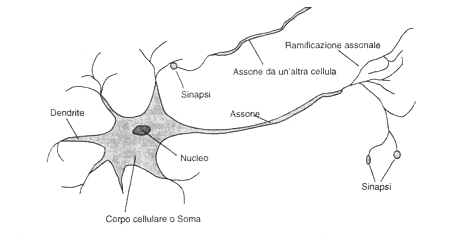
\includegraphics[width=\textwidth]{images/neuron.png}
	\caption{Neuroni biologici}\label{fig:neuron}
\end{figure}

All’estremità l'assone si ramifica formando terminali attraverso i quali i segnali elettrici vengono trasmessi ad altre cellule (ad esempio ai dendriti di altri neuroni). Tra un terminale di un assone e la cellula ricevente esiste uno spazio. I segnali superano questo spazio per mezzo di sostanze chimiche dette \emph{neurotrasmettitori}. Il punto di connessione tra terminale e dendrite è detto \textbf{sinapsi}.

\newpage
La trasmissione di un segnale nella corteccia cerebrale è un processo complesso.
In maniera molto semplificata, tale processo si compone delle seguenti fasi:
\begin{enumerate}
	\item Il corpo cellulare esegue una somma pesata dei segnali in ingresso;
	\item Se il risultato supera un certo valore soglia allora si produce un \textbf{potenziale d'azione}; una scarica di impulsi elettrici, che viene inviata all'assone. In questo caso, si dice che la cellula ``spari'' altrimenti non fa nulla;
	\item Quando il segnale elettrico raggiunge la sinapsi, viene rilasciato chimicamente un “neuro trasmettitore” che sarà combinato con i “recettori” nella membrana post-sinaptica (vedi Figura~\ref{fig:synapse});
	\item I recettori post-sinaptici provocano una diffusione del segnale elettrico nel neurone post-sinaptico.
\end{enumerate}

\begin{figure}[h!]
	\centering
	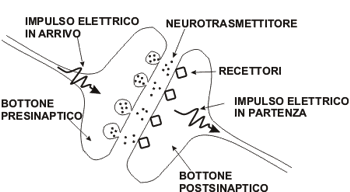
\includegraphics[width=8cm]{images/synapse.png}
	\caption{La sinapsi}\label{fig:synapse}
\end{figure}
\emph{L'apprendimento} si attua modificando la cosiddetta \textbf{efficacia sinaptica}, ovvero l'ammontare di corrente che entra nel neurone post-sinaptico rispetto al potenziale d'azione del neurone pre-sinaptico. In questo contesto le sinapsi possono essere: \textbf{eccitatorie}, nel senso che favoriscono la generazione di potenziale d'azione nel neurone post-sinaptico, oppure \textbf{inibitorie} che, invece, ne limitano la generazione.
Il cervello umano è un calcolatore complesso, non lineare e parallelo. Pur essendo costituito da elementi di elaborazione molto semplici (i neuroni), è in grado di eseguire computazioni complesse, come il riconoscimento, la percezione e il controllo del movimento, molte volte più velocemente del più veloce degli attuali calcolatori.\\

Nel cervello non esiste un controllo centralizzato, nel senso che le varie zone del cervello funzionano insieme, influenzandosi reciprocamente e contribuendo alla realizzazione di uno specifico compito.

\newpage

Infine, il cervello è \emph{fault tolerant}, cioè se un neurone o una delle sue connessioni sono danneggiati, il cervello continua a funzionare, anche se con prestazioni leggermente degradate. In particolare, le prestazioni del processo cerebrale degradano gradualmente man mano che si distruggono sempre più neuroni (\emph{graceful degradation}).
A tale scopo si sono studiate le caratteristiche del cervello umano.
Quindi, per riprodurre artificialmente il cervello umano occorre realizzare una rete di elementi molto semplici che sia una struttura \textbf{distribuita}, massicciamente \textbf{parallela}, capace di \textbf{apprendere} e quindi di \textbf{generalizzare} (cioè produrre uscite in corrispondenza di ingressi non incontrati durante l’addestramento).\\

Il metodo più usato per addestrare una rete neurale consiste nel presentare in ingresso alla rete un insieme di esempi (training set). La risposta fornita dalla rete per ogni esempio viene confrontata con la risposta desiderata, si valuta la differenza (errore) fra le due e, in base a tale differenza, si aggiustano i pesi. Questo processo viene ripetuto sull’intero training set finché le uscite della rete producono un errore al di sotto di una soglia prestabilita.\\

Anche se di recente introduzione, le reti neurali trovano valida applicazione in settori quali predizione, classificazione, riconoscimento e controllo, portando spesso contributi significativi alla soluzione di problemi difficilmente trattabili con metodologie classiche.

\newpage

\section{Modello di McCulloch e Pitts} % (fold)
\label{sec:modello_di_mcculloch_e_pitts}
Si introduce ora un modello artificiale del neurone biologico. Il neurone artificiale ha molti ingressi ed una sola uscita. Ogni ingresso ha associato un peso, che determina la conducibilità del canale di ingresso. L’attivazione del neurone è una funzione della somma pesata degli ingressi.

\begin{figure}[h!]
	\centering
	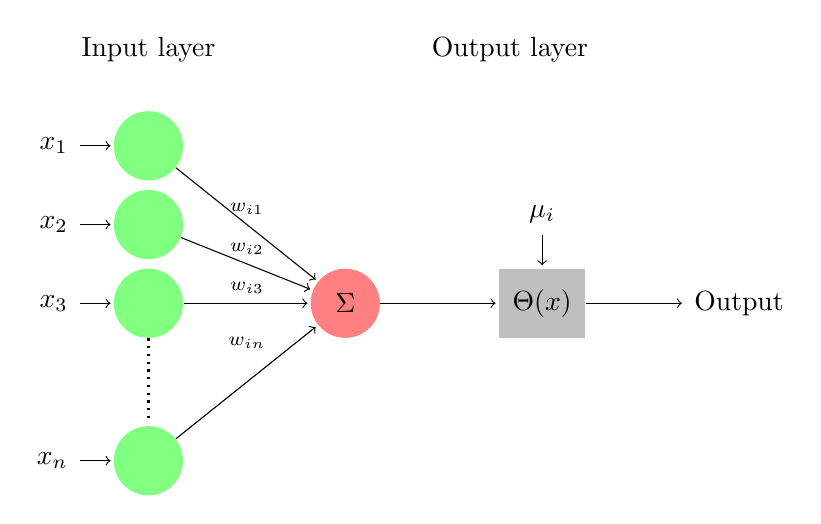
\begin{tikzpicture}[shorten >=1pt, node distance=\layersep]
		% Draw the input layer nodes
		\foreach \name / \y in {1,...,3}
		% This is the same as writing \foreach \name / \y in {1/1,2/2,3/3,4/4}
		\node[input neuron, pin=left:$x_\y$] (I-\name) at (0,-\y) {};
		\node[input neuron,  pin=left:$x_n$] (I-4) at (0,-5) {};
		\draw[dotted, thick] (I-3) -- (I-4);
		% Draw the output layer node
		\node[output neuron, right of=I-3] (O) {$\Sigma$};
		\node[neuron, rectangle, right of=O, inner sep=5pt, pin={[pin edge={<-}]above:$\mu_i$}] (F) {$\Theta(x)$};
		\node[right of=F] (Y) {Output};
		\path (O) edge [->] (F)
		(F) edge [->] (Y);
		% Connect every node in the hidden layer with the output layer
		\foreach \source in {1,...,3}
		\path (I-\source) edge [->, above] node {\scriptsize$w_{i\source}$} (O);
		\path (I-4) edge [->] node [above=0.3cm of I-4] {\scriptsize$w_{in}$} (O);
		\node[above=0.5cm of I-1] (In) {Input layer};
		\node[right=\layersep of In] {Output layer};
	\end{tikzpicture}
	\caption{Neurone artificiale nel modello M\&P}
\end{figure}

Un insieme di neuroni artificiali forma una \emph{rete artificiale}. Una rete neurale è un grafo diretto pesato $N=(V,E,w)$ dove $V=\{ 0,1,\dots, n\}$ è l'insieme delle unità (o neuroni), $E \subseteq V \times V$ è l'insieme di connessioni e $w:E \rightarrow \mathbb{R}$ è una funzione che assegna un peso con valore reale $w(i,j)$ per ogni connessione $(i,j)\in E$.\\

I pesi rappresentano l'efficacia sinaptica: pesi positivi amplificano il segnale, mentre quelli negativi lo inibiscono. Come notazione sarà utilizzata $w_{ij}$ anziché $w(i,j)$.\\

Un neurone si attiva se la somma pesata $\sum_j w_{ij} n_j$ degli input supera un certo valore soglia $\mu_i$. In termini matematici:
\begin{align}
	n_i(t + 1) = \Theta\left(\sum_j w_{ij} n_j(t) - \mu_i \right)
\end{align}

\newpage

Si tratta di un \textbf{modello semplificato} dove $\Theta(x)$ è la funzione di transizione o di attivazione ed in questo caso è discreta.
\begin{align}
	n_i(t + 1) =
	\begin{cases}
		1 & \mbox{if } \displaystyle\sum_j w_{ij} n_j \geq \mu_i \\
		0 & \mbox{otherwise} 
	\end{cases}
\end{align}

Anziché utilizzare una funzione discreta si possono adottare funzioni continue in modo tale da rendere il sistema più realistico. In questa caso l'output corrisponde alla frequenza delle volte in cui un neurone tramette. Esistono diverse funzioni di transizione continue; le più usate sono la sigmoidea e la tangente iperbolica.\\

\begin{figure}[h!]
	\begin{center}
		\subfigure[Tangente iperbolica]{
		\begin{tikzpicture}[domain=-1:1,scale=1.5]
			\draw[->] (-1,0) -- (1,0) node[right] {\tiny$x$};
			\draw[->] (0,-1.2) -- (0,1.2) node[above] {\tiny$f(x)$};
			\draw[dashed, thin] plot function{1} node[above]{\tiny +1};
			\draw[dashed, thin] plot function{-1} node[above]{\tiny-1};
			\draw[color=blue, thick] plot[id=tanh] function{tanh(x)};
		\end{tikzpicture}}
		\qquad
		\subfigure[Lineare]{
		\begin{tikzpicture}[domain=-1:1,scale=1.5]
			\draw[->] (-1,0) -- (1,0) node[right] {\tiny$x$};
			\draw[->] (0,-1.2) -- (0,1.2) node[above] {\tiny$f(x)$};
			\draw[dashed, thin] plot function{1} node[above]{\tiny +1};
			\draw[dashed, thin] plot function{-1} node[above]{\tiny-1};
			\draw[color=red, thick] plot[id=x] function{x};
		\end{tikzpicture}}
		\qquad
		\subfigure[Sigmoidea]{
		\begin{tikzpicture}[domain=-1:1,scale=1.5]
			\draw[->] (-1,0) -- (1,0) node[right] {\tiny$x$};
			\draw[->] (0,-1.2) -- (0,1.2) node[above] {\tiny$f(x)$};
			\draw[dashed, thin] plot function{1} node[above]{\tiny +1};
			\draw[color=orange, thick] plot[id=sigmoidal] function{1 / (1 +  exp(- 10 * x))};
		\end{tikzpicture}}
		\caption{Le funzioni di attivazione più utilizzate.}
	\end{center}
\end{figure}

Lo scopo delle funzioni di attivazione è ridurre la varianza in output di un neurone mappando il risultato della somma pesata entro un intervallo; generalmente compreso tra $[-1, 1]$ oppure $[0, 1]$.

\newpage

\subsection{Proprietà del modello M\&P} % (fold)
\label{sub:proprietà_del_modello}
Combinando opportunamente i neuroni di M\&P si possono costruire reti in grado di realizzare qualsiasi operazione del calcolo proposizionale.

\begin{figure}[h!]
	\centering

	\subfigure[AND]{
	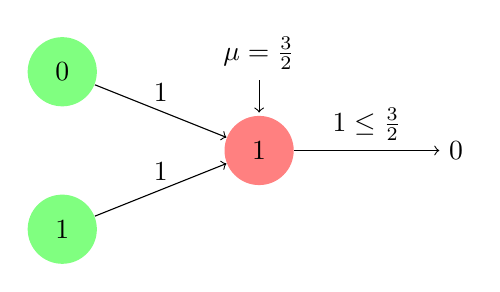
\begin{tikzpicture}[node distance=\layersep]]
		\node[input neuron] (I-1) at (0,1) {1};
		\node[input neuron] (I-2) at (0,3) {0};
		\node[output neuron, pin={[pin edge={<-}]above:$\mu=\frac{3}{2}$}, right of=I] (S) at (0,2) {1};
		\node[right of=S] (O) {0};
		\path 
		(I-1) edge[->] node[above] {1} (S)
		(I-2) edge[->] node[above] {1} (S)
		(S) edge[->] node[above] {$1 \leq \frac{3}{2}$} (O);
	\end{tikzpicture}}
	\qquad
	\subfigure[OR]{
	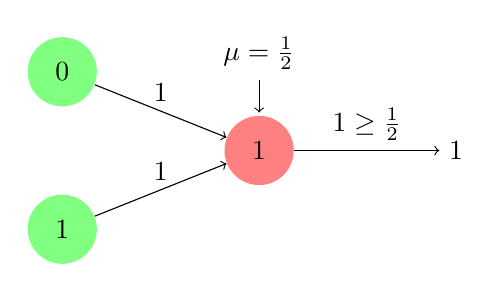
\begin{tikzpicture}[node distance=\layersep]]
		\node[input neuron] (I-1) at (0,1) {1};
		\node[input neuron] (I-2) at (0,3) {0};
		\node[output neuron, pin={[pin edge={<-}]above:$\mu=\frac{1}{2}$}, right of=I] (S) at (0,2) {1};
		\node[right of=S] (O) {1};
		\path 
		(I-1) edge[->] node[above] {1} (S)
		(I-2) edge[->] node[above] {1} (S)
		(S) edge[->] node[above] {$1 \geq \frac{1}{2}$} (O);
	\end{tikzpicture}}
	\subfigure[NOT]{
	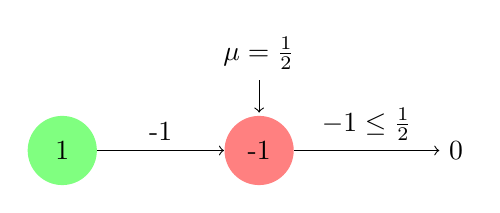
\begin{tikzpicture}[node distance=\layersep]]
        
		\node[input neuron] (I) {1};
		\node[output neuron, pin={[pin edge={<-}]above:$\mu=\frac{1}{2}$}, right of=I] (S) {-1};
		\node[right of=S] (O) {0};
		\path 
		(I) edge[->] node[above] {-1} (S)
		(S) edge[->] node[above] {$-1 \leq \frac{1}{2}$} (O);
	\end{tikzpicture}}
	\caption{Operazioni logiche elementari nel modello M\&P.}
\end{figure}

È importante notare che in questo modello \textbf{non} avviene ancora nessun tipo apprendimento. I pesi, infatti, rimangono fissi; l'apprendimento si realizza attraverso la variazione/aggiornamento dei pesi sinaptici.
% subsection proprietà_del_modello (end)
% section modello_di_mcculloch_e_pitts (end)

\newpage

\section{Tipi di architetture della rete} % (fold)
\label{sec:tipi_di_architetture_della_rete}
Il modo con cui è strutturata la rete dipende dall'algoritmo di apprendimento che si ha intenzione di usare. In generale si identificano tre classi di reti:
\begin{itemize}
	\item \textbf{reti feedforward ad uno strato}: In questa forma semplice di rete a strati, abbiamo i nodi di input (input layer) e uno strato di neuroni (output layer). Il segnale nella rete si propaga in avanti in modo aciclico, partendo dal layer di input e terminando in quello di output;
	\begin{figure}[h!]
		\centering
		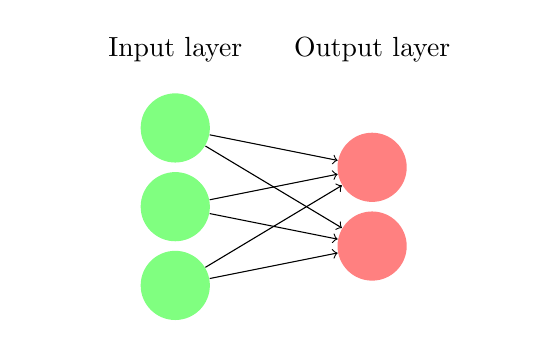
\begin{tikzpicture}[->, node distance=\layersep]

			% Draw the input layer nodes
			\foreach \name / \y in {1,...,3}
			\node[input neuron] (I-\name) at (0,-\y) {};

			% Draw the output layer nodes
			\foreach \name / \y in {1,...,2}   
			\node[output neuron] (O-\name) at (\layersep, -\y cm - 0.5cm) {};

			% Connect every node in the input layer with every node in the output layer.
			\foreach \source in {1,...,3}
			\foreach \dest in {1,...,2}
			\path (I-\source) edge (O-\dest);
                    
			% Annotate the layers
			\node[annot,above of=I-1, node distance=1cm] (il) {Input layer};
			\node[annot,right of=il] {Output layer};
		\end{tikzpicture}
		\caption{Rete forward ad uno strato}
	\end{figure}
    
	\item \textbf{reti feedforward a più strati:} questa classe di reti feedforward si distingue dalla precedente dal fatto che tra lo strato di input e quello di output abbiamo uno o più strati di neuroni nascosti (\textbf{hidden layers}).
	Questo tipo di architettura fornisce alla rete una prospettiva globale in quanto aumentano le interazioni tra neuroni;
	\begin{figure}[h!]
		\centering
		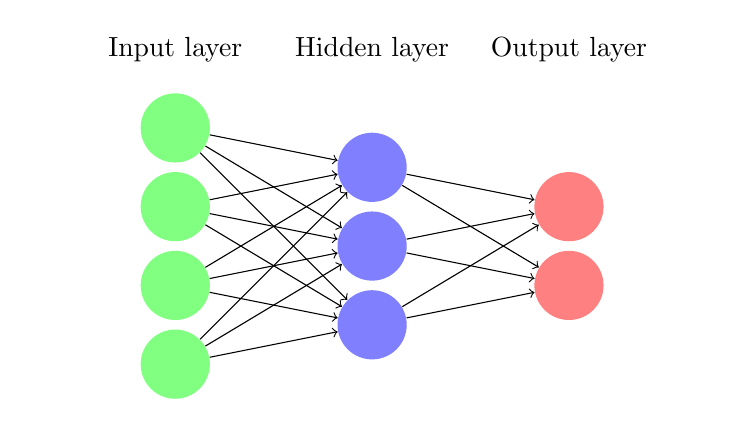
\begin{tikzpicture}[->, node distance=\layersep]

			% Draw the input layer nodes
			\foreach \name / \y in {1,...,4}
			\node[input neuron] (I-\name) at (0,-\y) {};

			% Draw the hidden layer nodes
			\foreach \name / \y in {1,...,3}
			\path[yshift=2cm]
			node[hidden neuron] (H-\name) at (\layersep, -\y cm - 2.5 cm) {};

			% Draw the output layer nodes
			\foreach \name / \y in {1,...,2}   
			\node[output neuron] (O-\name) at (2*\layersep, -\y cm - 1cm) {};

			% Connect every node in the input layer with every node in the hidden layer.
			\foreach \source in {1,...,4}
			\foreach \dest in {1,...,3}
			\path (I-\source) edge (H-\dest);
                    
			% Connect every node in the hidden layer with every node in the ouput layer.
			\foreach \source in {1,...,3}
			\foreach \dest in {1,...,2}
			\path (H-\source) edge (O-\dest);
                    
			% Annotate the layers
			\node[annot,above of=H-1, node distance=1.5cm] (hl) {Hidden layer};
			\node[annot,left of=hl] {Input layer};
			\node[annot,right of=hl] {Output layer};
		\end{tikzpicture}
		\caption{Rete forward a più strati}
	\end{figure}
    
	\newpage
    
	\item \textbf{reti feedback o ricorrenti}: una rete ricorrente si distingue dalle precedenti nel fatto che è ciclica. La presenza di cicli ha un impatto profondo sulle capacità di apprendimento della rete e sulle sue performance, in particolare rendono il sistema \textbf{dinamico}.
    
	\begin{figure}[h!]
		\centering
		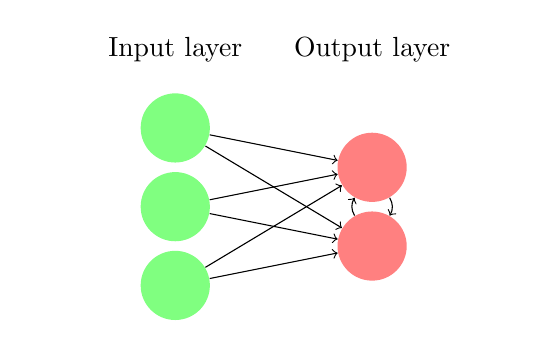
\begin{tikzpicture}[->, node distance=\layersep]

			% Draw the input layer nodes
			\foreach \name / \y in {1,...,3}
			\node[input neuron] (I-\name) at (0,-\y) {};

			% Draw the output layer nodes
			\foreach \name / \y in {1,...,2}   
			\node[output neuron] (O-\name) at (\layersep, -\y cm - 0.5cm) {};

			% Connect every node in the input layer with every node in the output layer.
			\foreach \source in {1,...,3}
			\foreach \dest in {1,...,2}
			\path (I-\source) edge (O-\dest);
                    
			% Connect every node in the output layer with every node in the ouptu layer.
			\foreach \source in {1,...,2}
			\foreach \dest in {1,...,2} 
			{
			\ifnum \source < \dest
			\path (O-\source) edge [bend left] (O-\dest);
			\fi
			\ifnum \source > \dest
			\path (O-\source) edge [bend left] (O-\dest);
			\fi
			}
			% Annotate the layers
			\node[annot,above of=I-1, node distance=1cm] (il) {Input layer};
			\node[annot,right of=il] {Output layer};
		\end{tikzpicture}
		\caption{Rete feedback.}
	\end{figure}
    
\end{itemize}
% section tipi_di_architetture_della_rete (end)
% chapter reti_neurali (end)

	%!TEX root = ../main.tex

\chapter{Problema di classificazione}
\label{cha:problema_di_classificazione}

In un tipico problema di classificazione si hanno a disposizione un insieme di \textbf{caratteristiche} $f_1, f_2, \dots,f_n$ e un insieme di \textbf{classi} $c_1, c_2, \dots, c_m$: l'obiettivo consiste nel classificare degli \emph{oggetti} in base alle loro caratteristiche. Un oggetto può essere rappresentato in uno spazio $n$-dimensionale e pertanto è possibile trattare problemi di classificazione attraverso metodi geometrici.

Lo spazio multidimensionale è suddiviso in \textbf{regioni di decisione}, ovvero aree all'interno delle quali ricadono tutti gli oggetti di una classe. I \textbf{confini} di queste regioni sono determinate dalla rete attraverso il processo di addestramento

Gli oggetti da classificare sono comunemente chiamati \textbf{pattern}. Una rete neurale impara a riconosce dei pattern a seguito di una \emph{fase di addestramento}, durante la quale alla rete vengono presentati un insieme di pattern di addestramento con l'indicazione della classe di appartenenza. Quando sarà presentato un nuovo pattern alla rete, appartenente ad una classeche questa ha precedentemente appreso, essa sarà in grado di classificarlo grazie alle informazioni estratte dai dati di addestramento.
\begin{figure}[h!]
	\centering
	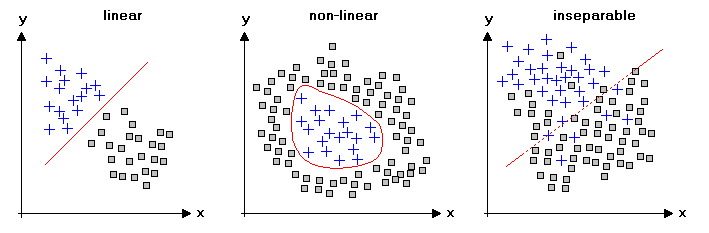
\includegraphics[width=\textwidth]{images/classify.png}
	\caption[Separabilità lineare nella classificazione.]{Rappresentazione geometrica di alcuni problemi di classificazione.}
\end{figure}

\noindent Quando si intende risolvere un problema di classificazione con una rete neurale, questa dovrà avere tante unità di input quante sono le caratteristiche degli oggetti e tanti neuroni di output quante sono le possibili classi.

\begin{figure}[h!]
	\centering
	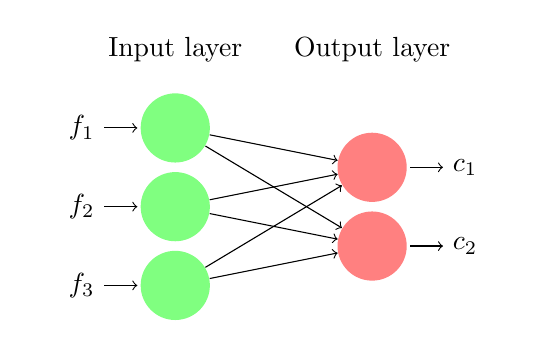
\begin{tikzpicture}[->, node distance=\layersep]

		% Draw the input layer nodes
		\foreach \name / \y in {1,...,3}
		\node[input neuron, pin=left:$f_\y$] (I-\name) at (0,-\y) {};

		% Draw the output layer nodes
		\foreach \name / \y in {1,...,2}   
		\node[output neuron, pin={[pin edge={->}]right:$c_\y$}] (O-\name) at (\layersep, -\y cm - 0.5cm) {};

		% Connect every node in the input layer with every node in the output layer.
		\foreach \source in {1,...,3}
		\foreach \dest in {1,...,2}
		\path (I-\source) edge (O-\dest);
                
		% Annotate the layers
		\node[annot,above of=I-1, node distance=1cm] (il) {Input layer};
		\node[annot,right of=il] {Output layer};
	\end{tikzpicture}
	\caption[Esempio di percettrone.]{Rete feedforward ad uno strato usata per la classificazione.}
\end{figure}

\newpage

\section{Percettrone a singolo strato}
\label{sec:percettrone_a_singolo_strato}
La prima rete neurale utilizzata per risolvere problemi di classificazione è il \textbf{percettrone} di Rosenblatt (1958), un classificatore \textbf{binario} caratterizzato da un singolo strato con connessioni feedforward.

Il percettrone è un idea semplice ed elegante: imita il neurone umano ed è in grado di imparare da esempi che gli vengono presentati. Tuttavia, come dimostrato da M. Minsky e S. Papert (1969), ha una pesante limitazione: è in grado di risolvere solo problemi \textbf{linearmente separabili}, ovvero problemi in cui le regioni di decisione si possono separare con un iperpiano.

\begin{figure}[h!]
	\centering
	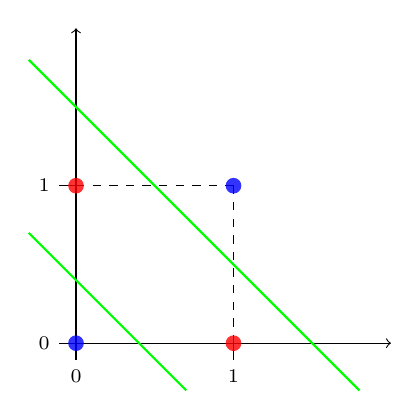
\begin{tikzpicture}[scale=2]
		
		% Axes
		\draw[->] (0,0) -- coordinate (x axis mid) (2,0);
		\draw[->] (0,0) -- coordinate (y axis mid) (0,2);
		
		% Ticks
		\foreach \x in {0,...,1}
		\draw (\x,1pt) -- (\x,-3pt)
		node[anchor=north] {\scriptsize\x};
		\foreach \y in {0,...,1}
		\draw (1pt,\y) -- (-3pt,\y)
		node[anchor=east] {\scriptsize\y};
		
		\draw[dashed] (1,0) -- (1,1);
		\draw[dashed] (0,1) -- (1,1);
		
		\draw[thick, color=green] (0.7,-0.3) -- (-0.3,0.7);
		\draw[thick, color=green] (-0.3,1.8) -- (1.8,-0.3);
		
		\node[fill=blue, circle, inner sep=2pt, opacity=0.8] at (0,0) {};
		\node[fill=red, circle, inner sep=2pt, opacity=0.8] at (0,1) {};
		\node[fill=red, circle, inner sep=2pt, opacity=0.8] at (1,0) {};
		\node[fill=blue, circle, inner sep=2pt, opacity=0.8] at (1,1) {};
		
		
	\end{tikzpicture}
	\caption{Non separabilità lineare dell'operatore XOR.}
\end{figure}

\noindent La convergenza del percettrone è garantita dal seguente teorema:
\begin{thm}[Teorema di convergenza del percettrone - N. J. Nilsson, 1965]
	Se il problema di classificazione è linearmente separabile allora la fase di apprendimento converge ad un'appropriata impostazione dei pesi in un numero finito di passi.
\end{thm}
Nella pratica non è dato sapere se un problema sia linearmente separabile o meno. La convergenza si può comunque ottenere aggiustando i parametri del percettrone come il numero di iterazioni o il fattore di apprendimento: in questo caso, tuttavia, la convergenza è artificiale.

\section{Percettrone a più strati}
\label{sec:percettrone_a_più_strati}

È possibile sopperire alle limitazioni dei percettroni a singolo strato aggiungendo strati di neuroni nascosti: il numero di strati, infatti, influenza la forma generale che possono assumere le regioni di decisione. Come si può osservare in figura \ref{fig:architetture}:
\begin{itemize}
	\item nelle reti a singolo strato si possono avere regioni di decisione separabili mediante un \textbf{iperpiano};
	\item nelle reti a due strati si possono avere \textbf{regioni convesse}, aperte o chiuse;
	\item nelle reti a tre strati le regioni possono avere forma arbitraria, la cui complessità dipende dal numero di neuroni nascosti.
\end{itemize}

\begin{figure}[h!]
	\centering
	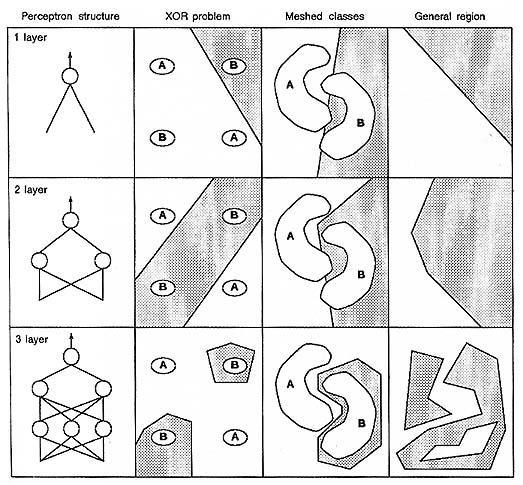
\includegraphics[width=10cm]{images/layers}
	\caption{Confronto tra architetture di rete.}
	\label{fig:architetture}
\end{figure}

\noindent Le potenzialità dei percettroni multistrato sono note da tempo, ma gli algoritmi per l'apprendimento sono stati ideati solo recentemente (1986).

\section{Previsione di serie temporali}
\label{sec:previsione_di_serie_temporali}

Le reti neurali, oltre alla classificazione e altri problemi \emph{discreti}, sono in grado di affrontare problemi \emph{continui} come la \textbf{previsione di una serie temporale}.

Si consideri una sequenza $P$ di vettori che dipendono dal tempo $t$:
\begin{align*}
	P = \{\vec{x}(t_0), \vec{x}(t_1), \cdots, \vec{x}(t_{i - 1}), \vec{x}(t_i), \vec{x}(t_{i + 1}), \cdots\}
\end{align*}
Per ottenere una serie $\{\vec{x}[t]\}$ da un segnale continuo $\vec{x}(t)$ è necessario \textbf{campionare} il segnale in punti discreti. 

Partendo da un tempo $t$ e procedendo a ritroso, otteniamo la serie temporale $\{\vec{x}[t], \vec{x}[t-1], \dots\}$. Lo scopo dell'analisi è di stimare $x(t)$ a un tempo futuro
\begin{align*}
	\hat{\vec{x}}[t+s] = f(\vec{x}[t], \vec{x}[t-1], \dots)
\end{align*}
dove $s$ è noto come \textbf{orizzonte della previsione}. Si tratta di un problema di approssimazione di una funzione che può essere risolto utilizzando una rete neurale a due strati.

\begin{thm}[Teorema dell'approssimazione universale - G. Cybenko, 1989 \& K. Hornik, 1991]
	Una rete neurale multistrato feed-forward con un singolo strato nascosto, un percettrone, che contiene un numero finito di neuroni nascosti è un approssimatore universale di funzioni continue su sottoinsiemi compatti $\mathbb{R}^n$.
\end{thm}

	%!TEX root = ../main.tex

\chapter{Algoritmo di back-propagation} % (fold)
\label{cha:algoritmo_di_back_propagation}
Il problema incontrato nell’addestramento delle reti multistrato è il seguente: volendo adottare un meccanismo di aggiornamento dei pesi simile a quello nelle reti a singolo strato (in cui l’errore è calcolato come differenza tra l’uscita desiderata e l’uscita effettiva di ciascun neurone) si riesce ad aggiornare solo i pesi relativi ai neuroni di uscita, ma non quelli relativi ai neuroni degli strati nascosti. Infatti, mentre per lo strato di uscita si conosce l’uscita desiderata (tale uscita viene data come secondo elemento delle coppie che costituiscono gli esempi del training set), niente si sa dell’uscita desiderata dai neuroni nascosti.\\

Questo problema è stato risolto dopo molti anni di disinteresse per le reti neurali (in quanto non si riusciva ad addestrarle) solo nel 1986, quando fu introdotto l’algoritmo di backpropagation. Tale algoritmo prevede di calcolare l’errore commesso da un neurone dell’ultimo strato nascosto propagando all’indietro l’errore calcolato sui neuroni di uscita collegati a tale neurone. Lo stesso procedimento è poi ripetuto per tutti i neuroni del penultimo strato nascosto, e così via.\\

L’algoritmo di backpropagation prevede che, per ogni esempio del training set, i segnali viaggino dall’ingresso verso l’uscita al fine di calcolare la risposta della rete. Dopo di che c’è una seconda fase durante la quale i segnali di errore vengono propagati all’indietro, sulle stesse connessioni su cui nella prima fase hanno viaggiato gli ingressi, ma in senso contrario, dall’uscita verso l’ingresso. Durante questa seconda fase vengono modificati i pesi.\\

I pesi sono inizializzati con valori casuali. Come funzione di uscita non lineare dei neuroni della rete si adotta in genere la funzione sigmoidea (l’algoritmo richiede che la funzione sia derivabile). L'algoritmo è basato sul metodo della \textbf{discesa del gradiente}.

\section{Metodo di discesa del gradiente} % (fold)
\label{sec:metodo_di_discesa_del_gradiente}

Il gradiente di una funzione $f$, denotato con $\nabla f$ è il vettore che ha come componenti le derivate parziali della funzione.
\begin{align}
	\nabla f(\bar{x}) = \left( \frac{\partial f(\bar{x})}{\partial x_1}, \frac{\partial f(\bar{x})}{\partial x_2}, \dots, \frac{\partial f(\bar{x})}{\partial x_n} \right)
\end{align}

La discesa del gradiente è una tecnica di ottimizzazione di tipo locale. Consiste nel valutare, inizialmente in un punto scelto a caso nello spazio multidimensionale (primo punto), sia la funzione stessa sia il suo gradiente.\\

Il gradiente indica la direzione in cui la funzione tende a un minimo/massimo, ovvero dove il gradiente tende a 0. Se si è interessati alla ricerca di un \textbf{minimo locale} si considerano i passi proporzionali al \emph{negativo} del gradiente della funzione nel punto corrente. Se, invece, si prendono i passi proporzionali al \emph{positivo} del gradiente si raggiungerà un \textbf{massimo locale}; la procedura in questo caso è nota come \emph{ascesa del gradiente}.\\

A titolo di esempio, il gradiente di $f(x, y) = x^2 + xy$ è:
\begin{align*}
	\nabla f(x, y) = \left\{\frac{df}{dx}, \frac{df}{dy} \right\} = \{2x + y, x\}
\end{align*}

% section metodo_di_discesa_del_gradiente (end)


\section{Apprendimento supervisionato} % (fold)
\label{sec:apprendimento_supervisionato}
L'algoritmo di backpropagation è un algoritmo di \emph{apprendimento supervisionato}, che prevede di presentare alla rete per ogni esempio di addestramento la corrispondente uscita desiderata.\\

Di solito i pesi vengono inizializzati con valori casuali all’inizio dell’addestramento. Poi si cominciano a presentare, uno alla volta, gli esempi costituenti l’insieme di addestramento (training set). Per ogni esempio presentato si calcola l’errore commesso dalla rete, cioè la differenza tra l’uscita desiderata e l’uscita effettiva della rete. L’errore è usato per aggiustare i pesi.\\

Il processo viene di solito ripetuto ripresentando alla rete, in ordine casuale, tutti gli esempi del training set finchè l’errore commesso su tutto il training set (oppure l’errore medio sul training set) risulta inferiore ad una soglia prestabilita.

\newpage

Dopo l’addestramento la rete viene testata controllandone il comportamento su un insieme di dati, detto test set, costituito da esempi non utilizzati durante la fase di training. La fase di test ha quindi lo scopo di valutare la capacità di generalizzazione della rete neurale. Si dice che la rete ha imparato, cioè è in grado di fornire risposte anche per ingressi che non le sono mai stati presentati durante la fase di addestramento.\\

Ovviamente le prestazioni di una rete neurale dipendono fortemente dall’insieme di esempi scelti per l’addestramento. Tali esempi devono quindi essere rappresentativi della realtà che la rete deve apprendere e in cui verrà utilizzata. L’addestramento è in effetti un processo ad hoc dipendente dallo specifico problema trattato.\\

Tecnicamente, è necessario un insieme di addestramento $L$ della forma: 
\begin{align}
	L = \{(\bar{x}_1, \bar{y}_1), \dots, (\bar{x}_p, \bar{y}_p) \}
\end{align}
dove
\begin{align*}
	&\bar{x}_\mu \mbox{ con $\mu=1, \dots, p$ è il vettore input} \\
	&\bar{y}_\mu \mbox{ con $\mu=1, \dots, p$ è il vettore dell'output desiderato}
\end{align*}

L'apprendimento consiste nel trovare una configurazione di pesi tale che l'output della rete sia il più vicino possibile all'output desiderato per tutti gli esempi presenti nel training set.\\

Formalmente, si tratta di trovare una configurazione di pesi tra tutte le possibili combinazioni $\overline{W}$ che minimizzi la seguente \emph{funzione di errore}. Essa dipende dal vettore $\mu$-esimo di output $out_\mu$ restituito dalla rete, dato il vettore $\mu$-esimo di ingresso $\overline{x}_\mu$ e dal vettore $\mu$-esimo di output $\overline{y}_\mu$ del training set. In termini matematici:
\begin{align*}
	\min_{\bar{w} \in \overline{W}} E(\bar{w}) &= \frac{1}{2} \sum_{\mu=1}^p \| \underbrace{\bar{y}_\mu}_\textrm{desiderato} - \underbrace{out_\mu (\bar{w})}_\textrm{reale} \|_2^2 \\
	&= \frac{1}{2} \sum_{\mu=1}^p \sum_{k=1}^n \left(y_k^\mu - out_k^\mu (\bar{w})\right)^2
\end{align*}
dove l'indice $k$ rappresenta il valore corrispondente al k-esimo neurone di output e il termine $1/2$ è aggiunto per cancellare l'esponente durante la derivazione.
% section apprendimento_supervisionato (end)

\newpage

\section{Propagazione dell'errore} % (fold)
\label{sec:back_propagation}
La funzione $E$ è altamente non lineare pertanto il problema di ottimizzazione non è facile da risolvere. Per minimizzare la funzione si utilizza il metodo della discesa del gradiente. Per calcolare le derivate parziali $\partial E / \partial w_{ij}$ è necessario l'algoritmo di back propagation. L'algoritmo può essere diviso in due passi:
\begin{itemize}
	\item \emph{Forward pass:} l'input dato alla rete è propagato al livello successivo e così via ai livelli successivi (il flusso di informazioni si sposta in avanti, cioè forward). Si calcola dunque $E(\bar{w})$, l'errore commesso.
	\item \emph{Backward pass:} L'errore fatto dalla rete è propagato all'indietro (backward) e i pesi sono aggiornati in maniera appropriata.
\end{itemize}
Il seguente schema descrive il funzionamento dell'algoritmo di retroazione.
\begin{figure}[h!]
	\centering
	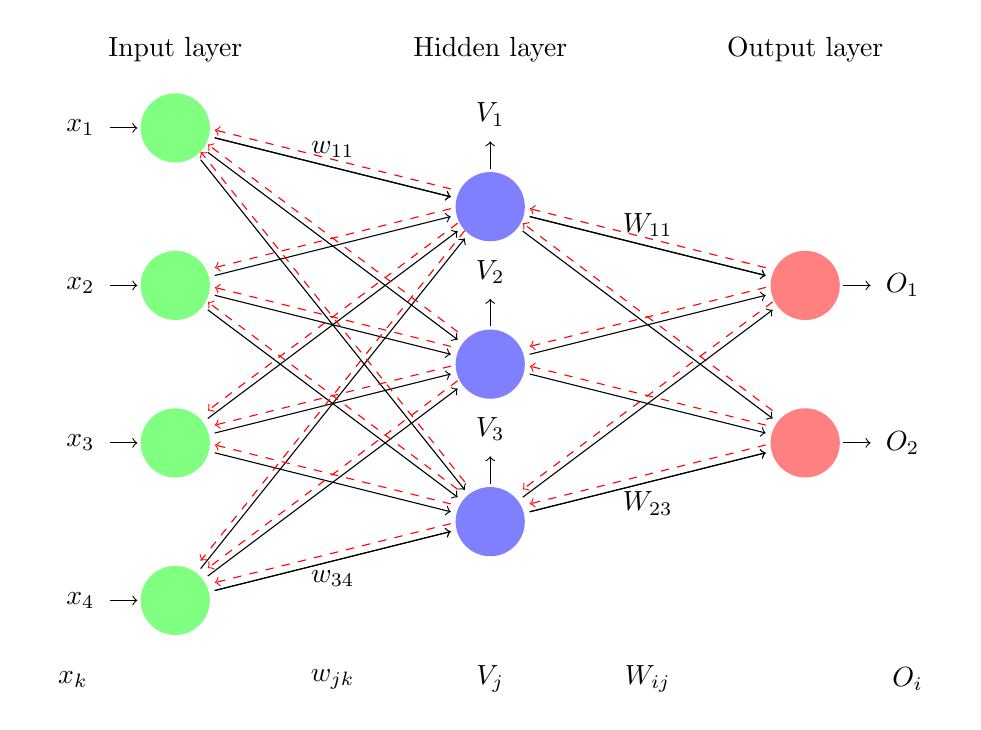
\begin{tikzpicture}[->,shorten >=2pt, shorten <= 2pt, auto, node distance=\layersep]
		\def\nodesep{-2cm}
		\def\layersep{4cm}
		% Draw the input layer nodes
		\foreach \name / \y in {1,...,4}
		\node[input neuron, pin=left:$x_\y$] (I-\name) at (0, \nodesep * \y) {};

		% Draw the hidden layer nodes
		\foreach \name / \y in {1,...,3}   
		\node[hidden neuron, pin={[pin edge={->}] above:$V_\y$}] (H-\name) at (\layersep, \nodesep * \y - 1 cm) {};
            
		% Draw the output layer nodes
		\foreach \name / \y in {1,...,2}   
		\node[output neuron, pin={[pin edge={->}]right:$O_\y$}] (O-\name) at (2*\layersep, \nodesep * \y - 2cm) {};

		% Connect every node in the input layer with every node in the hidden layer.
		\foreach \source in {1,...,4}
		\foreach \dest in {1,...,3}
		\path (I-\source) edge (H-\dest);

		% Error edges.
		\foreach \source in {1,...,4}
		\foreach \dest in {1,...,3}
		\path (H-\dest) edge[dashed, color=red, transform canvas={yshift=1mm}] (I-\source);

		\foreach \source in {1,...,3}
		\foreach \dest in {1,...,2}
		\path (O-\dest) edge[dashed, color=red, transform canvas={yshift=1mm}] (H-\source);


		\path (I-1) edge[above] node {$w_{11}$} (H-1);
		\path (I-4) edge[below] node {$w_{34}$} (H-3);
		% Connect every node in the hidden layer with every node in the output layer.
		\foreach \source in {1,...,3}
		\foreach \dest in {1,...,2}
		\path (H-\source) edge (O-\dest);


		\path (H-1) edge[above] node {$W_{11}$} (O-1);
		\path (H-3) edge[below] node {$W_{23}$} (O-2);
        
		% Annotate the layers
		\node[annot,above of=H-1, node distance=2cm] (hl) {Hidden layer};
		\node[annot,left of=hl] {Input layer};
		\node[annot,right of=hl] {Output layer};
        
		\node at (-1.3, - 9) {$x_k$};
		\node at (2, - 9) {$w_{jk}$};
		\node at (4, - 9) {$V_j$};
		\node at (6, - 9) {$W_{ij}$};
		\node at (9.3, - 9) {$O_i$};
        
	\end{tikzpicture}
	\caption[Schema back-propagation]{Schema back-propagation: le linee nere indicano il segnale propagato in avanti, mentre quelle rosse indicano l'errore propagato all'indietro.}\label{fig:backpro}
\end{figure}

Considereremo un metodo semplice che aggiorna i pesi di pattern in pattern fino al raggiungimento di un'epoca. \textbf{Un'epoca} è un ciclo di presentazione di tutti gli esempi del training set.
L'aggiustamento dei pesi viene fatto in base all'errore calcolato per ogni pattern presentato alla rete.
\newpage

Si definiscono ora, in termini matematici, gli input e gli output prodotti dai neuroni nascosti e di output.
Dato un pattern $\mu$, l'unità nascosta $j$ riceve un input netto dato da:
\begin{align}
	h_j^\mu = \sum_k w_{jk} x^\mu_k
\end{align}
e produce come output:
\begin{align}
	V_j^\mu = g(h_j^\mu) = g\left(\sum_k w_{jk} x^\mu_k \right)
\end{align}
Dove $g$ è la funzione di attivazione. In modo analogo il segnale entrante nell'unità output $i$ è definito come:
\begin{align}
	h_i^\mu = \sum_j W_{ij} \cdot V^\mu_j
\end{align}
E l'output prodotto $O_i$ è:
\begin{align}
	O_i = g(h^\mu_i) = g\left(\sum_j W_{ij} V^\mu_j \right)
	\end{align} 
	I pesi sono aggiornati nella direzione opposta rispetto al gradiente; siamo infatti interessati a trovare un minimo per la funzione $E$. Quindi i pesi all'iterazione $t + 1$ sono così calcolati:
	\begin{align*}
		w^{t+1} = w^t - \eta \cdot \nabla (E(w^t))
	\end{align*}


	Il parametro $\eta$ noto come \textbf{fattore di apprendimento} ha una forte influenza sul comportamento dell'algoritmo (velocità di convergenza, oscillazioni, ecc..).

	\begin{figure}[h!]
		\centering
		\begin{tikzpicture}
			\node[draw,circle,inner sep=1pt,fill] (1) at (0, 0) {};
			\node[above right=1mm of 1] {$w^t$};
			\node[draw,circle,inner sep=1pt,fill] (2) at (2, -1) {};
			\node[above right=1mm of 2] {$w^{t+1}$};
			\node (3) at (4, -2) {};
			\draw[->] (2) -- (3);
			\node[below=0.1mm of 3] {$-\nabla (E(w^t))$};
			\path (1) edge[very thick, below] node {$\eta$} (2);
		\end{tikzpicture}
		\caption{Direzione di aggiornamento dei pesi.}
	\end{figure}

	\newpage

	\subsection{Aggiornamento pesi strato nascosto-output} % (fold)
	\label{sub:aggiornamento_pesi_strato_nascosto_output}

	Calcoliamo ora la variazione di peso sinaptico tra il neurone di output $i$ e il neurone nascosto $j$ per un certo pattern $\mu$ del training set. Da notare come nella Figura~\ref{fig:backpro} utilizziamo la $W$ maiuscola per indicare i pesi tra il layer nascosto e quello ouput.
	\begin{align*}
		\Delta W_{ij} &= - \eta \cdot \frac{\partial E}{\partial W_{ij}} \\
		&= - \eta \cdot \frac{\partial}{\partial W_{ij}}\left[\frac{1}{2} \sum_\mu \sum_k (y_k^\mu - O_k^\mu)^2 \right]\\
		&= - \eta \cdot \sum_\mu \sum_k (y_k^\mu -O_k^\mu) \cdot \left( -  \frac{\partial O_k^\mu} {\partial W_{ij}} \right) = \eta \cdot \sum_\mu \sum_k (y_k^\mu -O_k^\mu) \frac{\partial O_k^\mu}{\partial W_{ij}} \\
		&\text{Per $k\neq i$, $O_k$ non dipende da $W_{ij}$, quindi la derivata per $O_k$ è 0;} \\
		&\text{ad esempio vedi Figura~\ref{fig:backpro} il peso $W_{11}$ non influenza $O_2$. } \\
		&= \eta \cdot \sum_\mu  (y_i^\mu - O_i^\mu) \frac{\partial O_i^\mu}{\partial W_{ij}} \\
		&= \eta \cdot \sum_\mu  (y_i^\mu - O_i^\mu) \cdot g'(h_i^\mu) \cdot \frac{\partial h_i^\mu}{\partial{W_{ij}}}
	\end{align*}
	Calcoliamo la derivata di $\partial h_i^\mu / \partial W_{ij}$:
	\begin{align*}
		\frac{\partial h_i^\mu}{\partial{W_{ij}}} &= \frac{\partial}{\partial{W_{ij}}} \sum_l V_l^\mu \cdot W_{il} \\
		& \text{Come prima per $l\neq j$ la derivata di $h^\mu_i$ è 0} \\
		&= \frac{\partial}{\partial{W_{ij}}} V_j^\mu \cdot W_{ij} = V_j^\mu
	\end{align*}
	Quindi:
	\begin{align*}
		\Delta W_{ij} = \eta \cdot \sum_\mu  (y_i^\mu - O_i^\mu) \cdot g'(h_i^\mu) \cdot V_j^\mu = \eta \cdot \sum_\mu \delta^\mu_i V^\mu_j
	\end{align*}
	Dove:
	\begin{align*}
		\delta^\mu_i = (y^\mu_i - O^\mu_i) g'(h^\mu_i)
	\end{align*}
	è l'errore del neurone $i$-esimo ed è noto come \textbf{gradiente locale}.
	% subsection aggiornamento_pesi_strato_input_nascosto (end)
	\newpage

	\subsection{Aggiornamento pesi strato input-nascosto} % (fold)
	\label{sub:aggiornamento_pesi_strato_input_nascosto}
	Si passa ora al calcolo della variazione di peso sinaptico tra il neurone nascosto $j$ e il neurone di input $k$ per un certo pattern $\mu$ del training set.
	\begin{align*}
		\Delta w_{jk} &= - \eta \cdot \frac{\partial E}{\partial w_{jk}} \\
		&= \eta \cdot \sum_\mu \sum_i (y^\mu_i - O^\mu_i)  \frac{\partial O^\mu_i}{\partial w_{jk}} \\
		&= \eta \cdot \sum_\mu \sum_i (y^\mu_i - O^\mu_i) \cdot   g'(h^\mu_i) \frac{\partial h^\mu_i}{\partial w_{jk}}
	\end{align*}
	In questo caso la seconda sommatoria rimane in quanto l'output dipende indirettamente dall'input; ad esempio il segnale entrante in $O_1$ dipende indirettamente da $w_{jk}$.
	Calcoliamo ora $\partial h^\mu_i / \partial w_{jk}$:
	\begin{align*}
		\frac{\partial h^\mu_i}{\partial w_{jk}} &= \sum_l W_{il} \frac{\partial V_l^\mu}{\partial w_{jk}} \\
		&\text{Come prima per $l\neq j$, $V_l$ non dipende da $w_{jk}$.} \\
		&= W_{ij} \frac{\partial V_j^\mu}{\partial w_{jk}} \\
		&= W_{ij} \frac{\partial g(h^\mu_j)}{\partial w_{jk}} \\
		&= W_{ij} g'(h^\mu_j) \frac{\partial h^\mu_j}{\partial w_{jk}}
	\end{align*}
	La derivata di $\partial h^\mu_j / \partial w_{jk}$ è:
	\begin{align*}
		\frac{\partial h^\mu_j}{\partial w_{jk}} 
		&= \frac{\partial}{\partial w_{jk}} \sum_m w_{jm} x^\mu_m \\
		&\text{Come al solito per $m \neq k$ la derivata è 0.} \\
		&= \frac{\partial}{\partial w_{jk}} w_{jk} x^\mu_k\\
		&= x^\mu_k
	\end{align*}

	\newpage

	Quindi abbiamo:
	\begin{align*}
		\Delta w_{jk} &= \eta \cdot \sum_\mu \sum_i (y_i^\mu - O^\mu_i) \cdot g'(h^\mu_i) W_{ij} g'(h_j^\mu) x^\mu_k\\
		&= \eta \cdot \sum_\mu \sum_i \delta_i^\mu W_{ij} g'(h_j^\mu) x^\mu_k \\
		&= \eta \cdot \sum_\mu \hat{\delta}_j^\mu x^\mu_k
	\end{align*}
	% subsection aggiornamento_pesi_strato_nascosto_output (end)

	Dove:
	\begin{align*}
		\hat{\delta}_j^\mu = g'(h_j^\mu) \sum_i \delta^\mu_i W_{ij}
	\end{align*}
	è il gradiente locale del neurone nascosto $j$ e la sommatoria rappresenta l'errore medio sullo strato di output causato dal neurone $j$ dello strato nascosto.

	\newpage

	\subsection{In generale} % (fold)
	\label{ssub:in_generale}
	\begin{figure}[h!]
		\centering
		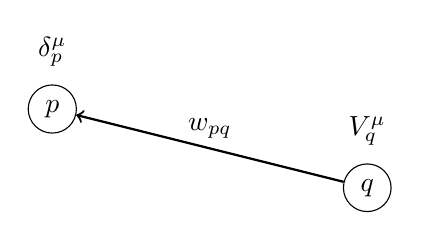
\begin{tikzpicture}
			\node[draw, circle] (1) at (0, 0) {$p$};
			\node[above=1mm of 1] {$\delta_p^\mu$};
			\node[draw, circle] (2) at (4, -1){$q$};
			\node[above=1mm of 2] {$V_q^\mu$};
        
			\path (1) edge[<-, thick, midway, above] node {$w_{pq}$} (2);
        
		\end{tikzpicture}
		\caption{Variazione di peso sinaptico.}
	\end{figure}

	In generale per l'aggiornamento dei pesi non sono necessarie informazioni globali, ma solo locali. La variazione di peso sinaptico tra un neurone $p$ e $q$ relativo ad un pattern $\mu$ del training set è dato da:
	\begin{align}
		\Delta w_{pq} = \eta \, \delta^\mu_p \, V^\mu_q
	\end{align}
	Dove:
	\begin{align*}
		\delta_p^\mu =
		\begin{cases}
			(y^\mu_p - O^\mu_p) \, g'(h^\mu_p), &\text{se $p$ è un neurone di output} \\
			\displaystyle g'(h_p^\mu) \, \sum_i \delta^\mu_i \, W_{ip} &\text{altrimenti}
		\end{cases}
	\end{align*}
	Questo modello prende il nome di apprendimento \textbf{on-line} in quanto la rete apprende un esempio alla volta. Esiste però un altro modello detto \textbf{off-line} o batch che considera tutti gli esempi dell'insieme di addestramento alla volta, anche se questo è meno coerente al modello biologico. Per l'apprendimento off-line abbiamo la seguente regola di apprendimento:
	\begin{align}
		\Delta w_{pq} = \eta \, \sum_\mu \delta^\mu_p \, V^\mu_q
	\end{align}

	% subsection in_generale (end)
	% section back_propagation (end)

	\newpage

	\section{I passi dell'algoritmo} % (fold)
	\label{sec:l'algoritmo}

	\algrenewcommand{\alglinenumber}[1]{\scriptsize\circled{#1}}% circled line numbers
	Si consideri una rete con $M$ strati e $m=0,\dots,M$. Si denota inoltre
	\begin{itemize}
		\item $V^m_i$: output della i-esima unità del livello m;
		\item $w^m_{ij}$: peso della connessione tra il j-esimo neurone dello strato $m-1$ e l'i-esimo neurone dello strato $m$. 
	\end{itemize}
	L'algoritmo di retroazione si compone dei seguenti passi:
	\begin{algorithmic}[1]% Taken from the algorithmicx package documentation
		\State Inizializzazione dei pesi a (piccoli) valori casuali;
		\State Scelta di un pattern $\overline{x}^\mu$ da inserire allo strato input $(m=0)$:
		\begin{align*}
			V^0_k = x^\mu_k \qquad \forall k
		\end{align*}
		\State Propagazione del segnale in avanti:
		\begin{align*}
			V^m_i = g(h_i^m) = g\left(\sum_j w_{ij} V_j^{m-1}\right)
		\end{align*}
		\State Calcolo degli errori $\delta$ dello strato output;
		\begin{align*}
			\delta^M_i = (y^M_i - V^M_i) \, g'(h^M_i)
		\end{align*}
		\State Calcolo degli errori $\delta$ per tutti gli strati precedenti;
		\begin{align*}
			\delta^{m-1}_i = g'\left(h^{m-1}_i\right) \, \sum_j \delta^m_j \, W_{ji}
		\end{align*}
		\State Aggiornamento dei pesi;
		\begin{align*}
			w^{NEW}_{ij} = w^{OLD}_{ij} + \Delta w_{ij} \qquad \text{dove } \Delta w_{ij} = \eta \delta_i^m V_j^{m-1} 
		\end{align*}
		\State Torna al passo 2 fino alla convergenza.
	\end{algorithmic}
	L'algoritmo si potrebbe fermare quando $\| w^{t+1} - w^t \| < \epsilon$ oppure dopo un certo numero di epoche se la condizione precedente non è rispettata.

	\newpage

	% section i_passi_dell'algoritmo (end)

	\section{Il momento} % (fold)
	\label{sub:il_momento}
	La scelta di $\eta$ influenza molto il comportamento dell'algoritmo, infatti se scegliamo valori troppo piccoli, la convergenza sarà lenta, mentre se si scelgono valori troppo grandi si rischia di avere una rete instabile con comportamento oscillatorio.
	Un metodo semplice per incrementare il fattore di apprendimento senza il rischio di rendere la rete instabile consiste nel modificare la regola di aggiornamento inserendo un nuovo termine: \emph{il momento}, una costante di proporzionalità alla precedente variazione dei pesi.
	\begin{align}
		\Delta w_{pq} (t + 1) = \underbrace{\alpha \Delta w_{pq} (t)}_\textrm{momento} - \eta \frac{\partial E}{\partial w_{pq}}
	\end{align}
	Dove $\alpha$ è un numero positivo a scelta preferibilmente compreso in $[0,1)$. In questo modo, il cambiamento dei pesi per l’esempio $t+1$ dipende dal cambiamento apportato ai pesi per l’esempio $t$.
	L'utilizzo del momento ha l'effetto di incrementare o decrementare l'ampiezza di aggiornamento in modo tale da \textbf{accellerare nelle discese} o \textbf{stabilizzare} l'algoritmo in caso di oscillazioni. Questo fatto ha, inoltre, il vantaggio di \textbf{prevenire} (non con certezza) che il processo di apprendimento incappi in minimi locali della funzione d'errore.

	\begin{figure}[h!]
		\centering
		\subfigure[Assenza di momento $\alpha=0$]{
		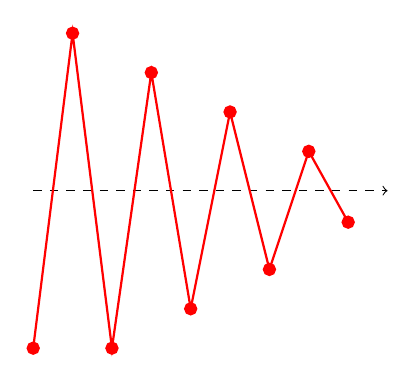
\begin{tikzpicture}
			\draw[->, dashed] (-2,0) -- (2.5,0);
			\draw[thick, color=red] plot [mark=*,red, tension=1.5] coordinates{
			(-2,-2) (-1.5, 2) (-1, -2) (-0.5, 1.5) (0, -1.5) (0.5, 1) (1, -1) (1.5, 0.5) (2, -0.4)};
		\end{tikzpicture}
		}
		\qquad
		\subfigure[Con momento $\alpha=0.5$]{
		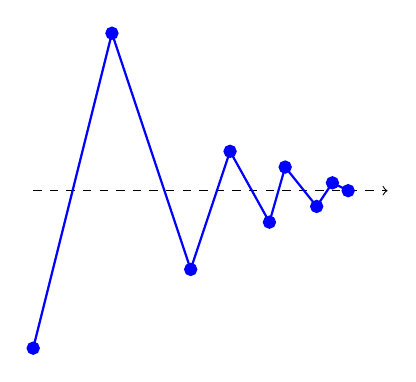
\begin{tikzpicture}
			\draw[->, dashed] (-2,0) -- (2.5,0);
			\draw[thick, color=blue] plot [mark=*,blue, tension=1.5] coordinates{
			(-2,-2) (-1, 2) (0, -1) (0.5, 0.5) (1, -0.4) (1.2, 0.3) (1.6, -0.2) (1.8, 0.1) (2, 0)};
		\end{tikzpicture}
		}
		\caption{Momento e discesa del gradiente su una semplice superficie.}
	\end{figure}

	% section il_momento (end)

	\newpage

	\section{Problema del minimo locale} % (fold)
	\label{sec:problema_del_minimo_locale}
	L'algoritmo di back-propagation non sempre è in grado di trovare il \emph{minimo globale}. Il problema risiede nell'esistenza di “buoni” o “cattivi” punti di minimo. Si consideri il seguente grafico:

	\begin{figure}[h!]
		\centering
		\begin{tikzpicture}
			% Axes
			\draw [->, name path=x] (-1,0) -- (12,0) node [right] {$x$};
			\draw [->] (0,-1) -- (0,6) node [above] {$y$};
			% Origin
			\node at (0,0) [below left] {$0$};
			% Points
			\coordinate (start) at (0,5);
			\coordinate (c1) at (2,2);
			\coordinate (c2) at (4,3);
			\coordinate (c3) at (6,1);
			\coordinate (c4) at (8,5);
			\coordinate (c5) at (10,4);
			\coordinate (end) at (12,5);
			% show the points
			%   \foreach \n in {start,c1,c2,c3,end} \fill [blue] (\n)
			%       circle (1pt) node [below] {\n};
			% join the coordinates
			\draw [thick,name path=curve] (start) to[out=0,in=180] (c1) to[out=0,in=180]
			(c2) to[out=0,in=180] (c3) to[out=0,in=180] (c4) to[out=0,in=180] (c5) to[out=0,in=180] (end);
			% add tangets and dashed lines
			\foreach \c / \name in {1/buon minimo locale,3/minimo globale, 5/pessimo minimo locale} {
			\draw [dashed] let \p1=(c\c) in (c\c) -- (\x1,0) node [below] {\name};
			\draw ($(c\c)-(0.75,0)$) -- ($(c\c)+(0.75,0)$) node [midway,above=4mm] {};
			}
		\end{tikzpicture}
		\caption{Rappresentazione del problema del minimo locale.}
	\end{figure}

	Per evitare il problema è importante scegliere una configurazione iniziale adeguata dei pesi. Se essi sono troppo elevati la derivata della funzione $g$ sarà vicina a zero e di conseguenza $\Delta w$ avrà valori molto piccoli. In questo modo il rischio di incappare in un minimo locale aumenta. Nella pratica si utilizza la seguente euristica per impostare i pesi iniziali:
	\begin{align*}
		w_{ij} \simeq \frac{1}{\sqrt{k_i}}
	\end{align*}
	dove $k_i$ è il numero di unità entranti nell'unità $i$.\\

	% section problema_del_minimo_locale (end)

	% chapter algoritmo_di_back_propagation (end)

	%!TEX root = ../main.tex

\chapter{Euristiche per migliorare l'apprendimento} % (fold)
\label{cha:euristiche_per_migliorare_l'apprendimento}
Per garantire la convergenza di un algoritmo di apprendimento non esistono criteri ben definiti. Ci sono una serie di questioni pratiche e teoriche da affrontare quando si vuole addestrare una rete neurale. Ad esempio: di quanti strati una rete dovrà essere composta, oppure, quante unità devono esserci per ogni strato. Per rispondere a queste domande si introduce il concetto di \textbf{generalizzazione}.

\section{Generalizzazione} % (fold)
\label{sec:generalizzazione}
\begin{mydef}[Generalizzazione]
	Per generalizzazione si intende la capacità di una rete di classificare correttamente esempi mai incontrati all'interno dell'insieme di addestramento (esempi di test).
\end{mydef}
Si assume che gli esempi di test siano tratti dalla stessa popolazione usata per generare il training set. Si introduce dunque un nuovo insieme noto come insieme dei test (\emph{test set}).\\

Il problema di apprendimento può essere visto come un problema di “approssimazione di una curva”. In questo caso la rete è considerata semplicemente come una mappa input/output non lineare, quindi una buona generalizzazione è vista come una buona interpolazione dei dati di input.\\

Una rete progettata per generalizzare bene produce mappature input/output corrette anche se l'input è lievemente differente dagli esempi usati in fase di training; se però la rete viene addestrata con troppi esempi, si rischia di memorizzare il training set; la rete cioè apprende il \emph{rumore} presente nel training set. Questo fenomeno è detto \textbf{overfitting} o \textbf{overtraining}. Una rete “sovra-addestrata” è troppo rigida e pertanto perde la capacità di generalizzazione.\\

\emph{In generale} una rete troppo piccola impara poco, mentre una rete troppo grande impara molto, ma non generalizza abbastanza. In entrambi i casi si rischia di non riuscire a risolvere il problema. È, dunque, necessario trovare un \textbf{giusto compromesso}. 

\newpage

Dal momento che stiamo considerando l'apprendimento come un'approssimazione di una curva, il compromesso precedente può essere visto sotto il seguente profilo: troppi pochi parametri e.g. $y=ax + b$ non permettono di risolvere il problema, mentre con troppi parametri e.g. $y=ax^3 + bx^2 + cx + d$ si rischia l'overfitting.

\begin{figure}[h!]
	\centering
	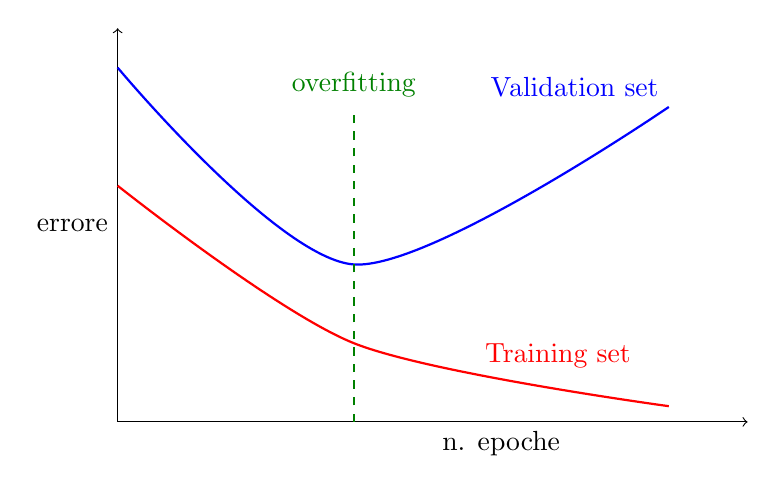
\begin{tikzpicture}
		\draw[->] (0,0) -- node[left] {errore} (0,5);
		\draw[->,below right] (0,0) -- node {n. epoche} (8,0);

		\draw[thick, color=blue] plot [smooth, tension=0.5] coordinates{(0, 4.5) (3, 2) (7, 4)} node[above left] {Validation set};
		\draw[thick, color=red] plot [smooth, tension=0.5] coordinates{(0, 3) (3, 1) (7, 0.2)} node[above left=0.5cm] {Training set};
        
		\draw[thick, color=green!50!black, dashed] (3, 0) -- (3, 4) node[above] {overfitting};
        
	\end{tikzpicture}
	\caption[Andamento dell'errore e overfitting]{La curva blu mostra l'andamento dell'errore nel classificare i dati di training, mentre la curva rossa mostra l'errore nel classificare i dati di test o validazione. Se l'errore di validazione aumenta mentre l'errore sui dati di training diminuisce, ciò indica che siamo in presenza di un possibile caso di overfitting.}
\end{figure}

\begin{figure}[h!]
	\centering
	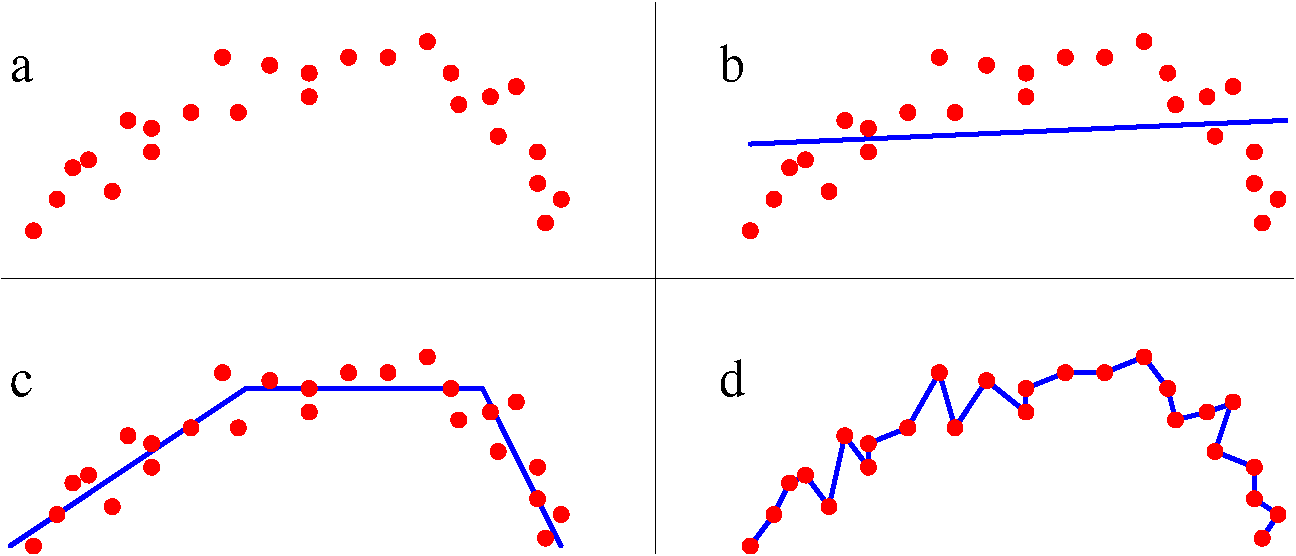
\includegraphics[width=10cm]{images/overfit2}
	\caption[Interpolazione e overfitting]{(a) dati del training set, (b) sotto approssimazione, (c) una buona stima sui dati, (d) overfitting: la curva di apprendimento è perfettamente disposta sul training set.}
\end{figure}

La capacità di generalizzazione è influenzata da tre fattori principali: le dimensioni del training set, l'architettura della rete neurale e la complessità del problema.

\newpage

Alla luce del fatto che non si ha alcun controllo sulla complessità del problema, è possibile affrontare il problema della generalizzazione sotto due punti di vista differenti:
\begin{enumerate}
	\item l'architettura della rete è prefissata e lo scopo è determinare una dimensione del training set ottimale per una buona generalizzazione;
	\item la dimensione del training set è prefissata e lo scopo è di determinare la migliore architettura di rete per una buona generalizzazione.
\end{enumerate}

% section generalizzazione (end)


\section{Cross-validation} % (fold)
\label{sec:cross_validation}
Si introduce ora uno strumento per risolvere il problema della selezione dell’architettura della rete neurale; più precisamente questo strumento consente, dato un insieme di possibili modelli, di scegliere quello migliore secondo certi criteri.
Inizialmente il set di dati viene ripartito in modo random in un training set e un test set. Il training set è ulteriormente diviso in due insiemi disgiunti:
\begin{itemize}
	\item \textbf{Estimation subset:} usato per il training del modello;
	\item \textbf{Validation subset:} usato per validare il modello.
\end{itemize}
La motivazione è validare il modello su un set di dati diverso da quello usato per l'addestramento. In questo modo è possibile usare il training set per stimare le prestazioni dei vari modelli candidati e scegliere quindi il migliore. C'è comunque la possibilità che il modello più performante in realtà sia incappato in un overfitting del validation set. Per evitare questo si ricorre al test set per verificare la capacità di generalizzazione della rete.

\newpage

\begin{figure}[h!]
	\centering
	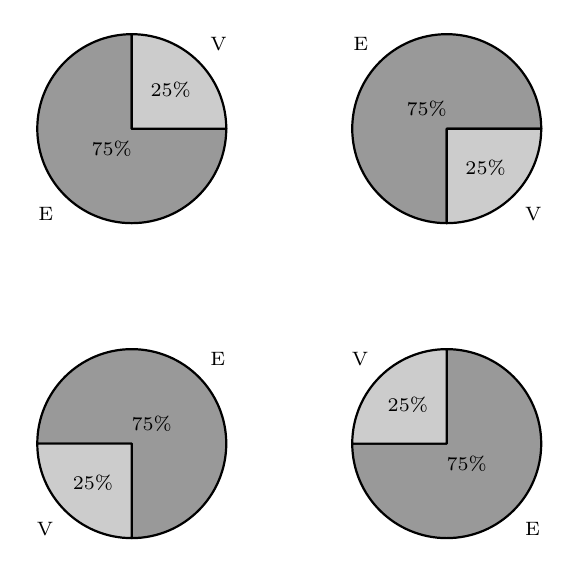
\begin{tikzpicture}[font=\scriptsize]
		\pie[pos={8,0},rotate=90, radius=1.2, color={black!40, black!20}]{75/ E, 25/ V}
		\pie[pos={12,0}, rotate=0, radius=1.2, color={black!40, black!20}]{75/ E, 25/ V}
		\pie[pos={8,-4}, rotate=270, radius=1.2, color={black!40, black!20}]{75/ E, 25/ V}
		\pie[pos={12,-4}, rotate=180, radius=1.2,  color={black!40, black!20}]{75/ E, 25/ V}
	\end{tikzpicture}
	\caption[Cross-validation]{Esempio di cross-validation: partizionamenti del training set in estimation subset E e validation subset V.}
\end{figure}

\subsection{Variante del cross-validation} % (fold)
\label{sub:variante_del_cross_validation}
Quando la dimensione del set di dati è piccola, si può ricorrere al \emph{multifold cross-validation} dividendo il set di $N$ esempi in $K$ sottoinsiemi, $K>1$. Il modello viene poi addestrato su ogni sottoinsieme ad eccezione di uno; quest'ultimo formerà il validation set. Questa procedura viene ripetuta $K$ volte utilizzando per il validation set a turno uno dei $K$ sottoinsiemi. Le prestazioni del modello vengono misurate facendo la media degli errori quadrati sul validation set per ognuna delle $K$ ripetizioni.\\
Lo svantaggio di questa tecnica è che richiede molta computazione dal momento che il modello deve essere addestrato $K$ volte.
Quando il numero di esempi è ancora più piccolo si può ricorrere ad una forma estrema di questa tecnica detta \textbf{leave-one-out} in cui $K=N$.
% subsection variante_del_cross_validation (end)
% section cross_validation (end)

\newpage

\section{Metodo di training “early-stopping”} % (fold)
\label{sec:metodo_di_training_early_stopping_}
Con l’obiettivo di una buona generalizzazione è molto difficile decidere quando è il momento di bloccare il training. C'è il rischio di overfitting dei dati se non si ferma l'addestramento al punto giusto.\\
È possibile evitare il fenomeno dell'overfitting ricorrendo al metodo precedente; l'estimation set viene usato per addestrare la rete e il validation set serve a testarla dopo ogni epoca. Più precisamente il processo procede nel seguente modo:
\begin{itemize}
	\item dopo un periodo di addestramento sull'estimation set, si calcola l'errore di validazione per ogni esempio del validation set;
	\item quando la fase di validazione è completa, si riprende la fase di addestramento per un altro periodo.
\end{itemize}

Se si osserva la sola curva dell'errore dell’estimation set (vedi Figura~\ref{fig:overfit}), questo si riduce all’aumentare delle epoche, e verrebbe naturale pensare di eseguire il training anche oltre il punto di minimo della curva del validation set. In realtà ciò che la rete apprende dopo quel punto è il rumore contenuto nei dati del training/estimation set. Questa euristica suggerisce quindi di fermare l'addestramento in corrispondenza del minimo della curva relativa al validation set.
\begin{figure}[h!]
	\centering
	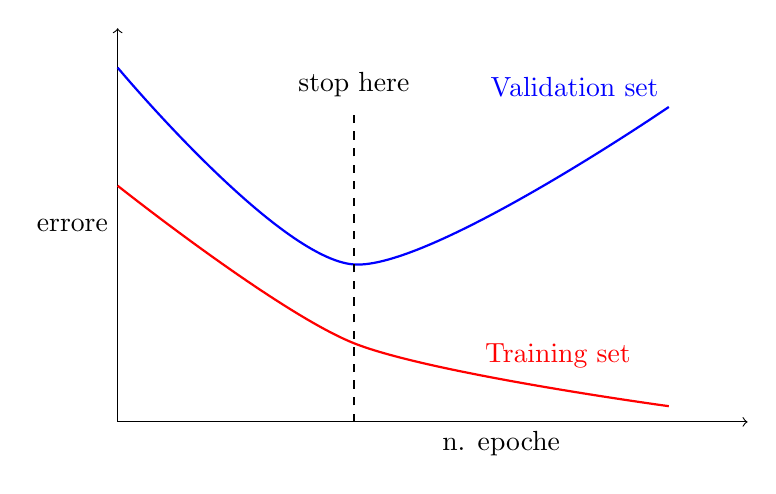
\begin{tikzpicture}
		\draw[->] (0,0) -- node[left] {errore} (0,5);
		\draw[->,below right] (0,0) -- node {n. epoche} (8,0);

		\draw[thick, color=blue] plot [smooth, tension=0.5] coordinates{(0, 4.5) (3, 2) (7, 4)} node[above left] {Validation set};
		\draw[thick, color=red] plot [smooth, tension=0.5] coordinates{(0, 3) (3, 1) (7, 0.2)} node[above left=0.5cm] {Training set};
        
		\draw[thick, dashed] (3, 0) -- (3, 4) node[above] {stop here};
        
	\end{tikzpicture}
	\caption{Andamento di errore e metodo di early stopping.}\label{fig:overfit}
\end{figure}



% section metodo_di_training_early_stopping_ (end)

\newpage

\section{Tecniche di pruning} % (fold)
\label{sec:tecniche_di_pruning}
Le capacità funzionali e di generalizzazione di una determinata rete sono fortemente influenzate dalla sua dimensione (ovvero il numero di neuroni nascosti). Con una rete troppo piccola si rischia di non riuscire a risolvere il problema, mentre con una troppo grande si rischia di apprendere il rumore deteriorando la capacità di generalizzare. È necessario quindi un \textbf{compromesso}.\\

Le tecniche di network pruning hanno lo scopo di minimizzare le dimensioni della rete mantenendo buone prestazioni. È possibile raggiungere questo obiettivo in due modi:
\begin{enumerate}
	\item \textbf{pruning}: si parte da una rete sufficientemente grande per poi ridurla eliminando connessioni sinaptiche o neuroni interi.
	\item \textbf{growing}: si parte da una rete piccola per poi espanderla;
\end{enumerate}
La prima tecnica di solito è più veloce in termini di numero di epoche (convergenza più veloce), ma richiede maggior peso computazionale dal momento che ci sono più unità. Ad ogni modo questo metodo è il più adottato.

\begin{figure}[h!]
	\centering
	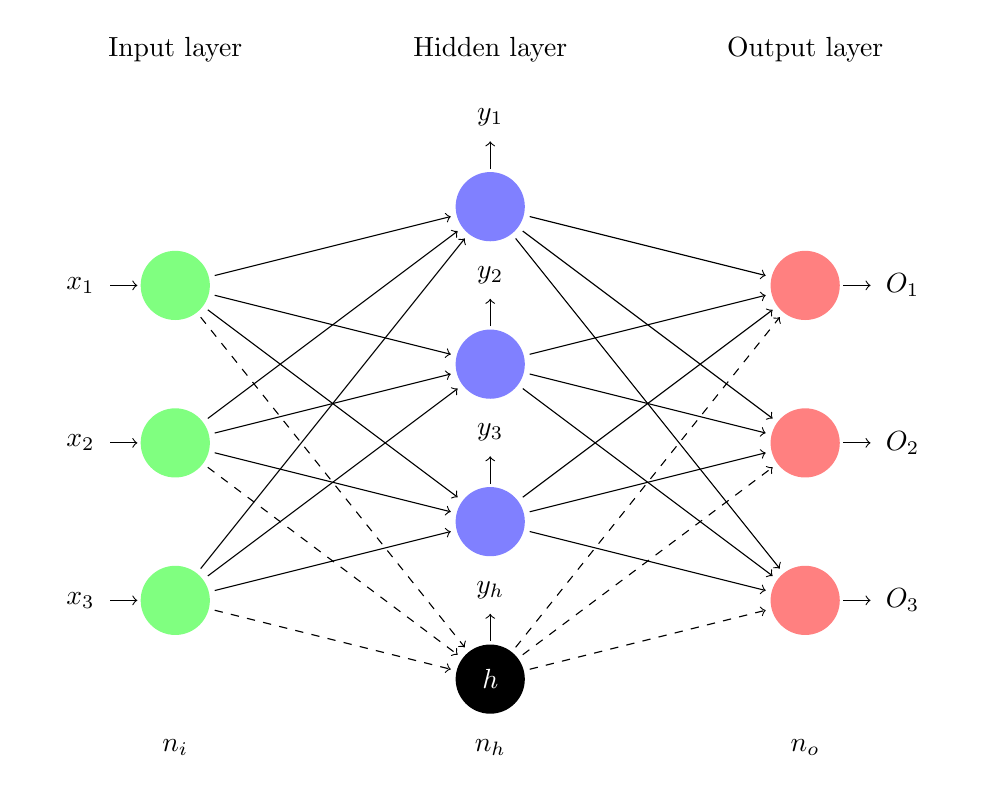
\begin{tikzpicture}[->,shorten >=2pt, shorten <= 2pt, auto, node distance=\layersep]
		\def\nodesep{-2cm}
		\def\layersep{4cm}
		% Draw the input layer nodes
		\foreach \name / \y in {1,...,3}
		\node[input neuron, pin=left:$x_\y$] (I-\name) at (0, \nodesep * \y) {};

		% Draw the hidden layer nodes
		\foreach \name / \y in {1,...,3}   
		\node[hidden neuron,  pin={[pin edge={->}] above:$y_\y$}] (H-\name) at (\layersep, \nodesep * \y + 1cm) {};
		
		\node[hidden neuron, color=black, text=white,  pin={[pin edge={->}] above:$y_h$}] (H-4) at (\layersep, \nodesep * 4 + 1cm) {$h$};
        
		% Draw the output layer nodes
		\foreach \name / \y in {1,...,3}   
		\node[output neuron, pin={[pin edge={->}]right:$O_\y$}] (O-\name) at (2*\layersep, \nodesep * \y) {};

		% Connect every node in the input layer with every node in the hidden layer.
		\foreach \source in {1,...,3}
		\foreach \dest in {1,...,3}
		\path (I-\source) edge (H-\dest);
                
		\foreach \source in {1,...,3}
		\path (I-\source) edge[dashed] (H-4);

		% Connect every node in the hidden layer with every node in the output layer.
		\foreach \source in {1,...,3}
		\foreach \dest in {1,...,3}
		\path (H-\source) edge (O-\dest);
                
		\foreach \source in {1,...,3}
		\path (H-4) edge[dashed] (O-\source);

		% Annotate the layers
		\node[annot,above of=H-1, node distance=2cm] (hl) {Hidden layer};
		\node[annot,left of=hl] {Input layer};
		\node[annot,right of=hl] {Output layer};
		\node[annot, below=2mm of H-4] (nh) {$n_h$};
		\node[annot, left of=nh] {$n_i$};
		\node[annot, right of=nh] {$n_o$};
	\end{tikzpicture}
	\caption{Rimozione del neurone $h$ in una rete neurale.}
\end{figure}

\newpage

L'approccio pruning consiste innanzitutto nel rimuovere un neurone $h$ e successivamente nell'aggiustare opportunamente i \emph{pesi entranti nelle unità servite dal neurone $h$} in modo tale da preservare il comportamento di input/output dell'intera rete.
In termini matematici si tratta di mantenere la seguente relazione:
\begin{align*}
	\underbrace{\sum_{j = 1}^{n_h}  w_{ij} y^\mu_j}_\textrm{prima} &= 
	\underbrace{\sum_{j = 1 \atop j \neq h} ^ {n_h} \left(w_{ij} + \delta_{ij} \right) y^\mu_j}_\textrm{dopo} \qquad \forall i = 1, \dots, n_o, \quad \forall \mu = 1, \dots, P
\end{align*}

dove $\delta_{ij}$ sono i fattori di aggiustamento che dovranno essere calcolati e $y_j^\mu$ indica l'output dell'unità $j$ corrispondente a un certo pattern $\mu$.
Attraverso procedimenti algebrici l'equazione precedente può essere riscritta nel seguente modo:
\begin{align*}
	\sum_{j = 1}^{n_h}  w_{ij} y^\mu_j = 
	\sum_{j = 1 \atop j \neq h} ^ {n_h} w_{ij} y^\mu_j + 
	\sum_{j = 1 \atop j \neq h} ^ {n_h} \delta_{ij} y^\mu_j
\end{align*}
E quindi rimane:
\begin{align*}
	\sum_{j = 1 \atop j \neq h} ^ {n_h} \delta_{ij} y^\mu_j =
	w_{ih} y^\mu_h
\end{align*}

che è un tipico sistema lineare di equazioni con incognite $\{\delta_{ij}\}$. È possibile porre tale sistema in forma compatta:
\begin{align*}
	A \bar{x} = b
\end{align*}
dove $A$ è la matrice di dimensione $n_o \times n_o (n_h - 1)$ e le cui colonne sono i vettori output delle unità servite da $h$. Dal momemto che il sistema è sovradeterminato (ci sono più equazioni che incognite) si può utilizzare il metodo dei minimi quadrati per approssimare una soluzione:
\begin{align}
	\min_{\bar{x}} \|A \bar{x} - b\|
\end{align}
I fattori di aggiustamento così calcolati permettono di preservare il comportamento della rete avendo rimosso il neurone $h$. Uno dei problemi fondamentali dell'algoritmo pruning è come meglio selezionare le unità che saranno rimosse. Idealmente, la scelta più appropriata sarebbe eliminare tutte le unità nascoste che hanno il più piccolo \emph{residuo finale} calcolato dal sistema corrispondente.

\newpage

Questo garantisce che la rimozione dell'unità avrà un impatto minimo sul comportamento della rete. Tuttavia, il calcolo del residuo minimo finale ha un costo computazionale piuttosto elevato (a causa del numero di soluzioni del sistema), pertanto nella pratica si cerca una soluzione ottimale utilizzando metodi di riduzione dei residui: si parte da una soluzione iniziale $x_0$ e si produce una sequenza di punti $\{ x_k \}$ tale che i residui si riducono: 
\begin{align*}
	\|A \bar{x} - b\| = r_k
\end{align*}
dove $r_0 \geq r_1 \geq \dots \geq r_k \geq r_{k + 1}$. Un'approssimazione accettabile alla soluzione ottimale globale sarebbe scegliere l'unità $h$ da eliminare in modo tale che il \emph{residuo iniziale} sia il più piccolo. Dal momento che $x_0$ di solito è il vettore nullo allora:
\begin{align*}
	x_0 = 0 \implies r_0 = \| b \|
\end{align*}
Si tratta quindi di scegliere l'unità con $\| b \|$ minimo. Naturalmente questo criterio non garantisce la soluzione ottimale globale in quanto non è detto che partendo dal residuo iniziale minimo si giunga al residuo finale minimo. Tuttavia, nella pratica, questo criterio si è dimostrato efficace e semplice da implementare.\\

Riassumendo i passi fondamentali dell'algoritmo di pruning sono i seguenti:
\begin{algorithmic}[1]% Taken from the algorithmicx package documentation
	\State Data una rete sovradimensionata;
	\State Ripetere:
	\begin{enumerate}[(a)]
		\item Trovare l'unità $h$ con $\| b \|$ minimo;
		\item Risolvere il sistema corrispondente (aggiustare i pesi);
		\item Rimuovere l'unità $h$.
	\end{enumerate}
	Fino a quando $Performance(pruned) - Performance(original) < \epsilon$
	\State Rifiuta la rete ridotta.
\end{algorithmic}




% section tecniche_di_pruning (end)

% chapter euristiche_per_migliorare_l'apprendimento (end)
















	%!TEX root = ../main.tex

\chapter{Reti di Hopfield}
\label{cha:reti_di_hopfield}

In questo capitolo considereremo le reti neurali viste come \textbf{sistemi dinamici}\footnote{Un sistema dinamico è un modello matematico utilizzato per descrivere situazioni il cui stato varia nel tempo.} non lineari, con particolare attenzione al problema della loro stabilità o neurodinamica (vedi appendice~\ref{cha:sistemi_dinamici}): per introdurre la variabile tempo in una rete è sufficiente aggiungere dei cicli, ovvero operare con \textbf{reti ricorrenti}.

Le reti ricorrenti con unità non lineari sono generalmente difficili da analizzare: possono convergere a uno stato stabile, oscillare o seguire \textbf{traiettorie caotiche} il cui andamento non è prevedibile.

Tuttavia, il fisico americano J. J. Hopfield si accorse che se le connessioni sono \textbf{simmetriche} esiste una funzione di \textbf{energia globale}. Le reti di Hopfield sono:
\begin{itemize}
	\item \textbf{reti ricorrenti ad uno strato} in cui ogni neurone è connesso a tutti gli altri (escluso sè stesso);
	\item \textbf{simmetriche}: perché hanno la matrice dei pesi sinaptici simmetrica, ovvero $\mat{W}=\mat{W}^T$;
	\item \textbf{non lineari}: nella formulazione continua, ogni neurone ha una funzione di attivazione non lineare invertibile.
\end{itemize}

\begin{figure}[h!]
	\centering
	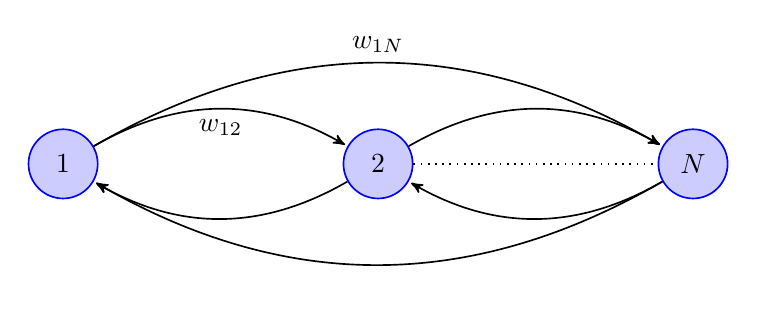
\begin{tikzpicture}[->,>=stealth',shorten >=1pt,auto,node distance=4cm, semithick]
		\tikzstyle{every state}=[align=center, fill=blue!20,draw=blue]
		
		% Draw nodes.
		\node[state] (1) {$1$};
		\node[state, right of=1] (2) {$2$};
		\node[state, right of=2] (N) {$N$};
        
		% Draw edges
		\path 
		(1) edge[bend left, below] node {$w_{12}$} (2)
		(1) edge[bend left] node {$w_{1N}$} (N)
		(2) edge[bend left] (1)
		(2) edge[bend left] (N)
		(N) edge[bend left] (1)
		(N) edge[bend left] (2)
		(2) edge[dotted, -] (N);
        
	\end{tikzpicture}
	\caption{Una rete ricorrente.}
\end{figure}

\noindent Per quanto riguarda l'aggiornamento di un neurone si possono scegliere tre strade diverse:
\begin{itemize}
	\item \textbf{aggiornamento asincrono}, in cui si aggiorna un neurone alla volta;
	\item \textbf{aggiornamento sincrono}, dove tutti i neuroni vengono aggiornati nello stesso istante;
	\item \textbf{aggiornamento continuo}, in cui tutti i neuroni si aggiornano continuamente.
\end{itemize}
Esistono infine due formulazioni del modello di Hopfield, \textbf{discreto} e \textbf{continuo}, che si differenziano per la modalità di scorrimento del tempo.

\begin{figure}[h!]
	\centering
	\subfigure[Caso discreto: $\Delta t$ costante]{
	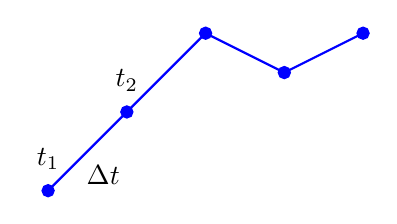
\begin{tikzpicture}
		\draw[thick, color=blue] plot [mark=*,blue, tension=1]
		coordinates{(0, 0) (1, 1) (2, 2) ( 3, 1.5) (4, 2)};
		\node[] at (0, 0.4) {$t_1$};
		\node[] at (0.7, 0.2) {$\Delta t$};
		\node[] at (1, 1.4) {$t_2$};
	\end{tikzpicture}}
	\quad
	\subfigure[Caso continuo: $\Delta t \rightarrow 0$]{
	\begin{tikzpicture}
		\draw[thick, color=blue] plot [smooth, red, tension=1]
		coordinates{(0, 0) (2, 2) ( 3, 1.5) (4, 2)};
	\end{tikzpicture}}
	\caption{Confronto tra caso discreto e continuo.}
\end{figure}

\section{Modello di Hopfield: caso discreto}
\label{sec:modello_di_hopfield_caso_discreto}

In questa sezione si considerano reti di Hopfield in cui il tempo scorre in maniera discreta e i neuroni si aggiornano in modo asincrono.

Per quanto riguarda l'input al neurone si adotta lo stesso modello di McCulloch e Pitts, con l'aggiunta di un fattore di influenza esterno:
\begin{displaymath}
	H_i = \underbrace{\sum_{j \neq i} w_{ij} V_j}_\textrm{modello M\&P} + \underbrace{I_i}_\textrm{input esterno}
\end{displaymath}
La funzione di attivazione (discreta) è la seguente:
\begin{align}
	V_i = \begin{cases}
		+1 & \text{se } H_i > 0 \\
		-1 & \text{se } H_i < 0
	\end{cases}\label{eq:learningrule}
\end{align}
L'aggiornamento dei neuroni è un processo casuale e la selezione dell'unità da aggiornare può essere fatta in due modi:
\begin{enumerate}
	\item ad ogni istante temporale si sceglie a caso l'unità $i$ da aggiornare (utile nelle simulazioni);
	\item ogni unità si aggiorna indipendentemente con probabilità costante ad ogni istante.
\end{enumerate}
A differenza delle reti feedforward, una rete di Hopfield è un sistema dinamico: parte da uno stato iniziale
\begin{align*}
	\vec{V}(0) = (V_1(0), \dots, V_n(0))^T
\end{align*}
ed evolve lungo una traiettoria fino a raggiungere un punto fisso in cui $\vec{V}(t+1) = \vec{V}(t)$ (convergenza).
\begin{figure}[h!]
	\centering
	\begin{tikzpicture}
		\node[point] (0) at (-4, 0) {};
		\node[point] (1) at (-2, 2) {};
		\node[point] (2) at (0, -0.4) {};
		\node[point] (3) at (2, 1) {};
		\node[point] (4) at (4, 0) {};
		\node[point] (5) at (6, -0.5) {};
		\node[point] (6) at (8, 0.5) {};
         
		\foreach \x / \y in {0/1,1/2,2/3,3/4,4/5,5/6}
		\path (\x) edge[->] (\y);
         
		\foreach \x in {0,...,6}
		\node[above=2mm of \x] {\small$\vec{V}(\x)$};
         
	\end{tikzpicture}
	\caption{Traiettoria di una rete di Hopfield nel modello discreto.}
\end{figure}

\noindent Per dimostrare la convergenza, introduciamo la \textbf{funzione di energia} $E$ che governa il sistema
\begin{align}
	E = - \frac{1}{2} \sum_{i=1}^n \sum_{\substack{j=1 \\ j \neq i}}^n w_{ij} V_i V_j - \sum_{i=1}^n I_i V_i\label{eq:energy}
\end{align}
dove il fattore $1/2$ è aggiunto perché i termini identici $w_{ij}x_i x_j$ e $w_{ji} x_j x_i$ sono presenti nella doppia sommatoria.

Il seguente teorema fornisce una condizione sufficiente per la convergenza del sistema.
\begin{thm}[Teorema di Hopfield (caso discreto) - J. J. Hopfield, 1982]
	Se la matrice dei pesi di una rete di Hopfield è simmetrica con $\diag(\mat{W}) = \vec{0}$, allora la funzione di energia \eqref{eq:energy} è una funzione di Lyapunov per il sistema, quindi
\begin{displaymath}
	\Delta E = E(t+1) - E(t) \leq 0
\end{displaymath}
con uguaglianza solo quando il sistema ha raggiunto un punto stazionario.
\end{thm}

\begin{proof}[Dimostrazione.]
	Visto che stiamo utilizzando la modalità di aggiornamento asincrono, supponiamo che il neurone $h$ cambi il proprio stato. La differenza di energia è data da:
	\begin{alignat*}{2}
		\Delta E &=&& - \frac{1}{2} \sum_{i=1}^n \sum_{\substack{j=1 \\ j \neq i}}^n w_{ij} V_i(t + 1) V_j(t + 1) - \sum_{i=1}^n I_i V_i(t + 1) \\
		&&& + \frac{1}{2} \sum_{i=1}^n \sum_{\substack{j=1 \\ j \neq i}}^n w_{ij} V_i(t) V_j(t) + \sum_{i=1}^n I_i V_i(t) \displaybreak[3]\\
		&=&& \underbrace{- \frac{1}{2} \sum_{i=1}^n \sum_{\substack{j=1 \\ j \neq i}}^n w_{ij} (V_i(t + 1) V_j(t + 1) - V_i(t) V_j(t))}_\textbf{$A$} \\
		&&& \underbrace{- \sum_{i=1}^n I_i (V_i(t + 1) - V_i(t))}_\textbf{$B$}
	\end{alignat*}
	Per quanto riguarda il termine $B$ abbiamo:
	\begin{align*}
		B &= - \sum_{i=1}^n I_i \Delta V_i \\
		&= - I_h \Delta V_h
	\end{align*}
	Passiamo ora al primo termine $A$; per prima cosa espandiamo la sommatoria isolando il neurone $h$:
	\begin{align*}
		A =& \underbrace{- \frac{1}{2} \sum_{i \neq h} \sum_{j \neq i} w_{ij} (V_i(t + 1) V_j(t + 1) - V_i(t) V_j(t))}_\textrm{$A_1$} \\
		& \underbrace{- \frac{1}{2} \sum_{j \neq h} w_{hj} (V_h(t + 1) V_j(t + 1) - V_h(t) V_j(t))}_\textrm{$A_2$}
	\end{align*}
	Poiché $V_i(t) = V_i(t + 1)$ per $i \neq h$ si può riscrivere $A_1$ come:
	\begin{align*}
		A_1 &= - \frac{1}{2} \sum_{i \neq h} \sum_{j \neq i} w_{ij} (\underbrace{V_i(t + 1)}_\textrm{$=V_i(t)$} V_j(t + 1) - V_i(t) V_j(t)) \\
		&= - \frac{1}{2} \sum_{i \neq h} \sum_{j \neq i} w_{ij} V_i(t) \underbrace{(V_j(t + 1) - V_j(t))}_\textrm{$=\Delta V_j$} \\
		&= - \frac{1}{2} \sum_{i \neq h} w_{ih} V_i(t) \Delta V_h
	\end{align*}
	Per quanto riguarda $A_2$ il procedimento è lo stesso:
	\begin{align*}
		A_2 &= - \frac{1}{2} \sum_{j \neq h} w_{hj} (V_h(t + 1) V_j(t + 1) - V_h(t) V_j(t)) \\
		&= - \frac{1}{2} \sum_{i \neq h} w_{hi} V_i(t) \Delta V_h
	\end{align*}
	Siccome la matrice dei pesi è simmetrica si ha
	\begin{displaymath}
		A = A_1 + A_2 = - \Delta V_h \sum_{i \neq h} w_{ih} V_i(t)
	\end{displaymath}
	da cui:
	\begin{align*}
		\Delta E &= - \Delta V_h \sum_{i \neq h} w_{ih} V_i(t)  - I_h \Delta V_h \\
		&= - \Delta V_h \underbrace{\left[\sum_{i \neq h} w_{ih} V_i(t) + I_h \right]}_\textrm{input di $h$ al tempo $t + 1$} \\
		&= - \Delta V_h H_h(t + 1)
	\end{align*}
	A questo punto è necessario dimostrare che il prodotto $\Delta V_h H_h(t + 1)$ è sempre non negativo, in modo tale da provare la tesi. Per la regola di apprendimento \eqref{eq:learningrule} si ha
	\begin{enumerate}
		\item $\Delta V_h > 0$ se e solo se $H_h(t + 1) > 0$;
		\item $\Delta V_h < 0$ se e solo se $H_h(t + 1) < 0$;
	\end{enumerate}
	quindi il prodotto è sempre non negativo.
\end{proof}

\section{Regola di Hebb}

Nei computer, se si vuole accedere ad una certa informazione, si utilizza il suo preciso indirizzo di memoria: questo tipo di memoria è definita \textbf{byte-addressable memory}. Nel cervello umano, invece, la memoria è indirizzata in base al contenuto, \textbf{content-addressable memory}: ad esempio pensare alla parola \emph{volpe} potrebbe automaticamente attivare memorie relative ad altri animali simili, alla caccia, oppure al concetto di furbizia.

La \textbf{regola di Hebb} è stata introdotta per descrivere questo meccanismo di accesso alle informazioni e si basa sul principio che, se due neuroni si attivano contemporaneamente, la loro interconnessione deve essere rafforzata. In dettaglio il postulato di Hebb afferma:
\begin{quote}
	\emph{Quando un assone di un neurone A è abbastanza vicino da eccitare un neurone B e questo, in modo ripetitivo e persistente, gli invia un potenziale di azione, inizia un processo di crescita in uno o entrambi i neuroni tale da incrementare l'efficienza di A.}
\end{quote}
La memoria è rappresentata da un insieme di $P$ patterns $\vec{x}^\mu$, con $\mu = 1, \dots, P$: quando viene presentato un nuovo pattern $\vec{x}$, la rete tipicamente risponde producendo il pattern salvato in memoria che più somiglia a $\vec{x}$.

In accordo al postulato di Hebb, sono utilizzati pesi proporzionali alla correlazione nell'attivazione tra un neurone pre e post sinaptico
\begin{displaymath}
	w_{ij} = \frac{1}{N} \sum_{\mu = 1}^P x_i^\mu x_j^\mu
\end{displaymath}
dove $N$ è il numero di unità binarie con output $s_1, \dots, s_N$.

Il meccanismo di \textbf{recall} è il seguente:
\begin{displaymath}
	s_i = \sign\left(\sum_j w_{ij} s_j \right)
\end{displaymath}
Ci sono tuttavia alcuni problemi nell'utilizzo di reti di Hopfield come memorie indirizzate dal contenuto:
\begin{itemize}
	\item il numero massimo di pattern\footnote{I pattern sono memorizzati negli stati di equilibrio della rete.} è $0.15 N$;
	\item talvolta la rete produce degli \textbf{stati spuri}, ovvero stati che non fanno parte dei pattern memorizzati;
	\item il pattern evocato non è necessariamente il più simile a quello di input;
	\item i pattern non sono richiamati tutti con la stessa enfasi.
\end{itemize}

\section{Modello di Hopfield: caso continuo}
\label{sec:modello_di_hopfield_caso_continuo}

In questo modello i neuroni non sono più dispositivi binari con stati $(0, 1)$ o $(-1, 1)$, ma producono un output che identifica la quantità di corrente elettrica: lo scopo di Hopfield, infatti, era quello di fornire un'implementazione fisica del suo modello che imiti il più possibile il funzionamento di un cervello biologico.

L'output di un neurone $i$ è dato da
\begin{displaymath}
	V_i = g_\beta(\mu_i) = g_\beta \left(\sum_{j} w_{ij} V_j + I_i \right) 
\end{displaymath}
dove $g_\beta$ è la funzione di attivazione \textbf{crescente}, \textbf{continua} e \textbf{non lineare}. Le funzioni più utilizzate come $g_\beta$ sono la tangente iperbolica e la sigmoidea:
\begin{align*}
	\tanh_\beta(\mu) &= \frac {e^{\beta\mu} - e^{-\beta\mu}} {e^{\beta\mu} + e^{-\beta\mu}} \quad \in\; ]-1,1[ &
	g_\beta(\mu) &=\frac{1}{1 + e^{- \beta \mu}} \quad\in\; ]0,1[
\end{align*}
Il parametro $\beta$ indica la \emph{stickiness} della funzione: per $\beta \rightarrow \infty$ la funzione diventa sempre più ripida fino a diventare una funzione a gradino.

\begin{figure}[h!]
	\centering
	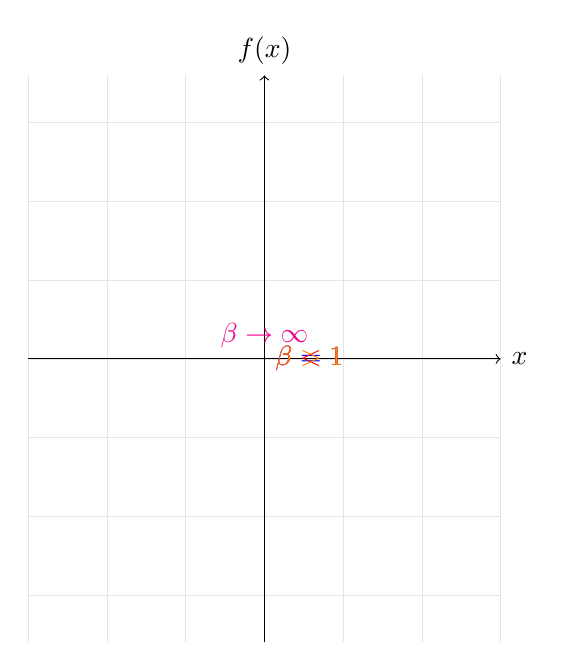
\begin{tikzpicture}[domain=-1:1,x=3cm,y=3cm,  every node/.style=very thick]
		\draw[very thin,color=gray!20] (-1,-1.2) grid (1,1.2);
		\draw[->] (-1,0) -- (1,0) node[right] {$x$};
		\draw[->] (0,-1.2) -- (0,1.2) node[above] {$f(x)$};
		\draw[color=blue] plot[id=tanh] function{tanh(1 * x)} node[right] {$\beta = 1$};
		\draw[color=red] plot[id=tanh] function{tanh(0.5 * x)} node[right] {$\beta < 1$};
		\draw[color=orange] plot[id=tanh] function{tanh(1.5 * x)} node[right] {$\beta > 1$};
		\draw[color=magenta] plot[id=tanh] function{tanh(100 * x)} node[above] {$\beta \rightarrow \infty$};
	\end{tikzpicture}
	\caption{La funzione tangente iperbolica.}\label{fig:stickiness}
\end{figure}

\noindent L'utilizzo di valori continui permette la modalità di \textbf{aggiornamento continuo} dei neuroni. Secondo questa modalità, il sistema evolve in accordo al seguente insieme di equazioni differenziali
\begin{displaymath}
	V_i + \tau_i \frac{\dif V_i}{\dif t} = g_\beta \left(\sum_{j} w_{ij} V_j + I_i \right)
\end{displaymath}
dove $\tau_i$ è una costante positiva che rappresenta la resistenza elettrica. Il sistema raggiunge la stabilità quando $\dif V_i / \dif t= 0 \, \forall i$.

In maniera del tutto equivalente, è possibile esprimere l'equazione di stato non incentrando l'attenzione sulla variazione dello stato $V_i$ nel tempo, quanto sulla variazione dell'input netto $\mu_i$ nel tempo, pervenendo alla seguente equazione:
\begin{displaymath}
	\mu_i + \tau_i \frac{\dif\mu_i}{\dif t} = \sum_j w_{ij} V_j + I_i = \sum_j w_{ij} g_\beta (\mu_j) + I_i \\
\end{displaymath}
La \textbf{funzione energia} nel modello continuo è simile a quella nel caso discreto:
\begin{align}
	E = - \frac{1}{2} \sum_i \sum_j w_{ij} V_i V_j + \sum_i \int_0^{V_i} g^{-1}_\beta (V) \, \dif V - \sum_i I_i V_i \label{eq:energycont}
\end{align}

\noindent Analogamente al caso discreto, il seguente teorema fornisce una condizione sufficiente per la convergenza del sistema.
\begin{thm}[Teorema di Hopfield (caso continuo) - J. J. Hopfield, 1982]
	Se la matrice dei pesi di una rete di Hopfield è simmetrica con $\diag(W) = \vec{0}$, allora la funzione di energia \eqref{eq:energycont} è una funzione di Lyapunov per il sistema, quindi $\dif E / \dif t \leq 0$ con uguaglianza quando il sistema ha raggiunto un punto stazionario.
\end{thm}

\begin{proof}[Dimostrazione.]
	Calcoliamo la derivata della funzione energia:
	\begin{align*}
		\frac{\dif E}{\dif t} &= - \frac{1}{2} \sum_i \sum_j w_{ij} \frac{\dif V_i}{\dif t} V_j - \frac{1}{2} \sum_i \sum_j w_{ij} V_i \frac{\dif V_j}{\dif t} + \sum_i \underbrace{g_\beta^{-1}(V_i)}_\textrm{$= \mu_i$} \frac{\dif V_i}{\dif t} - \sum_i I_i \frac{\dif V_i}{\dif t} \\
		\intertext{Per simmetria di $W$ si possono sommare i primi due termini:}
		&=  - \sum_i \sum_j w_{ij} \frac{\dif V_i}{\dif t} V_j + \sum_i \mu_i \frac{\dif V_i}{\dif t} - \sum_i I_i \frac{\dif V_i}{\dif t} \\
		&= - \sum_i \frac{\dif V_i}{\dif t} \underbrace{\left(\sum_j w_{ij} V_j - \mu_i + I_i \right)}_\textrm{$ = \tau_i \frac{\dif \mu_i}{\dif t}$} \\
		&= - \sum_i \tau_i \frac{\dif V_i}{\dif t} \frac{\dif \mu_i}{\dif t} \\
		&= - \sum_i \tau_i g'_\beta(\mu_i) \left(\frac{\dif \mu_i}{\dif t} \right)^2 \leq 0
	\end{align*}
	L'ultima disuguaglianza è verificata poiché $g_\beta$ è crescente, quindi $g'_\beta > 0$, $\tau_i > 0$ per ipotesi e il quadrato di un numero è sempre non negativo. Vale quindi la doppia implicazione
	\begin{align*}
		\frac{\dif E}{\dif t} = 0 \Leftrightarrow \frac{\dif \mu_i}{\dif t} = 0 \,\forall i
	\end{align*}
	cioè il valore dell'energia nel tempo rimane fisso se e solo se la rete ha raggiunto un punto di equilibrio.
\end{proof}

\section{Corrispondenza tra i due modelli}
\label{sec:corrispondenza_tra_i_due_modelli}

Esiste una relazione stretta tra il modello continuo e quello discreto. Si noti che
\begin{align*}
	V_i = g_\beta(\mu_i) = g_1(\beta \mu_i)
\end{align*}
da cui si ricava:
\begin{align*}
	\mu_i = \frac{1}{\beta} g_1^{-1} (V_i)
\end{align*}
Il secondo termine della funzione energia diventa
\begin{align*}
	\sum_i \int_0^{V_i} g_\beta^{-1}(V) \, \dif V = \frac{1}{\beta} \sum_i \int_0^{V_i} g_1^{-1}(V) \, \dif V 
\end{align*}
che, per $\beta \rightarrow \infty$, diventa trascurabile e la funzione di energia risulta uguale a quella nel modello discreto.
\begin{align*}
	E &= - \frac{1}{2} \sum_i \sum_j w_{ij} V_i V_j + \underbrace{\frac{1}{\beta}  \sum_i \int_0^{V_i} g_1^{-1} (V) \, \dif V}_\textrm{= 0 per $\beta \rightarrow \infty$}  - \sum_i I_i V_i \\
	&=  - \frac{1}{2} \sum_i \sum_j w_{ij} V_i V_j - \sum_{i=1}^n I_i V_i
\end{align*}

	%!TEX root = ../main.tex

\chapter{Ottimizzazione con le Reti Neurali} % (fold)
\label{cha:ottimizzazione_con_le_reti_neurali}
In questo capitolo saranno introdotti alcuni famosi problemi NP-Difficili: il problema del commesso viaggiatore (TSP) e il problema della cricca massima (MCP). Dal momento che questi non sono risolvibili in termini polinomiali sarà fornita una formulazione alternativa del problema in modo tale da poter utilizzare tecniche di ottimizzazione per approssimare una soluzione.

\section{Problema del commesso viaggiatore} % (fold)
\label{sec:problema_del_commesso_viaggiatore}
Il problema del commesso viaggiatore (in inglese “travelling salesman problem”) nasce dalla sua più tipica rappresentazione: data una rete di città, connesse tramite delle strade, trovare il percorso di minore lunghezza che un commesso viaggiatore deve seguire per visitare tutte le città una e una sola volta per poi tornare alla città di partenza.\\

Il problema è di considerevole importanza pratica, al di là delle ovvie applicazioni nella logistica e nei trasporti.


\subsection{Formulazione del problema} % (fold)
\label{sub:formulazione_del_problema}
Espresso nei termini della teoria dei grafi il TSP è così formulato: \emph{dato un grafo completo pesato $G=(V, E, w)$, trovare il cammino di costo minore visitando tutti i nodi $V$ una sola volta e tornando al nodo di partenza.}\\

La rete di città può essere rappresentata come un grafo in cui le città sono i nodi $V$, le strade gli archi $E$ e le distanze i pesi sugli archi $w$. La differenza sostanziale rispetto al Ciclo Hamiltoniano si trova nel fatto che quest'ultimo è formulato su di un grafo privo di pesi. Il problema è NP-completo: per poter trovare il percorso minimo è necessario elencare tutti gli \textbf{$n!$} percorsi.

\newpage

\begin{figure}[h!]
	\centering
	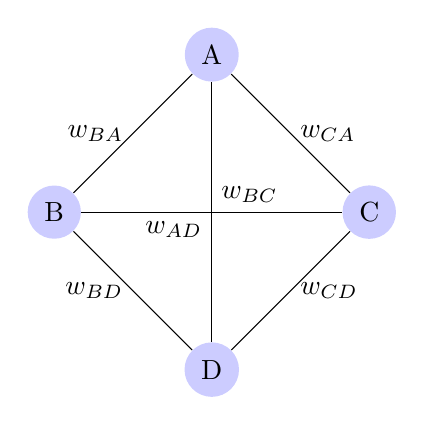
\begin{tikzpicture}
        
		\node[circle,fill=blue!20] (A) at (0,2) {A};
		\node[circle,fill=blue!20] (B) at (-2,0) {B};
		\node[circle,fill=blue!20] (C) at (2,0) {C};
		\node[circle,fill=blue!20] (D) at (0, -2) {D};
        
		\foreach \from / \to in {B/A,B/D}
		\path (\from) edge[left] node {$w_{\from\to}$} (\to);
        
		\foreach \from / \to in {C/A,C/D}
		\path (\from) edge[right] node {$w_{\from\to}$} (\to);
             
		\path (A) edge[below left=0.1cm  of A] node {$w_{AD}$} (D);
		\path (B) edge[above right=0.1cm  of C] node {$w_{BC}$} (C);
             
	\end{tikzpicture}
	\caption{Grafo completo pesato.}\label{fig:graph}
\end{figure}

% subsection formulazione_del_problema (end)

\subsection{Soluzione del TSP con le reti di Hopfield} % (fold)
\label{sub:soluzione_del_tsp_con_le_reti_di_hopfield}
È possibile affrontare questo problema utilizzando le reti di Hopfield. Per fare ciò è necessario \emph{trovare una funzione di energia $E$ adeguata in modo tale che il minimo corrisponda alla soluzione del problema che si sta affrontando.}\\

Per prima cosa è necessario rappresentare il TSP attraverso una matrice di permutazione per identificare un percorso. Ad esempio dato il grafo in Figura~\ref{fig:graph}, il percorso $B \rightarrow A \rightarrow C \rightarrow D$ può essere rappresentato con la seguente matrice:\\

\begin{table}[h!]
	\centering
	\begin{tabularx}{8cm}{lXXXX}
		\toprule
		\backslashbox{Città}{Fermata} & 1 & 2 & 3 & 4 \\
		\midrule
		A & 0 & \textbf{1} & 0 & 0 \\
		B & \textbf{1} & 0 & 0 & 0 \\
		C & 0 & 0 & \textbf{1} & 0 \\
		D & 0 & 0 & 0 & \textbf{1} \\
		\bottomrule
	\end{tabularx}
	\caption{Matrice di permutazione del percorso BACD}
\end{table}

Dunque per $n$ città saranno necessari $n \times n$ neuroni nella rete di Hopfield in cui ogni neurone identifica una città e una fermata.

\newpage

La soluzione del problema sarà dunque una matrice $V$ di dimensione $n \times n$. Si introducono ora alcune notazioni:
\begin{itemize}
	\item $X$ indica la città;
	\item $i$ una fermata in cui è visitata una città;
	\item $V_{X,i}$ è l'output dell'unità $X, i$;
	\item $T_{Xi, Yj}$ sono i pesi delle connessioni;
	\item $V_{X,i} = 1$ se la città $X$ è visitata alla fermata $i$;
	\item $d_{X,Y}$ distanza tra la città $X$ e $Y$.
\end{itemize}

Si definisce ora la funzione obiettivo da minimizzare che rappresenta il costo totale del cammino:
\begin{align*}
	E_1  = \frac{D}{2} \sum_X \sum_{Y \neq X} \sum_i d_{X,Y} V_{X,i} (V_{Y, i-1} + V_{Y, i+1})
\end{align*}
dove $D$ è una costante e gli indici sono intesi modulo $n$. La matrice $V$ senza vincoli di alcun genere può descrivere zero o più percorsi di lunghezza arbitraria (quindi può anche non toccare tutte le città).
Se la matrice $V$ descrivesse solo percorsi unici Hamiltoniani, allora minimizzando la funzione costo $E_1$ otterremmo la soluzione. Tuttavia il problema del commesso viaggiatore presenta una serie di \textbf{vincoli} che devono essere rispettati dalla matrice $V$.


\begin{figure}[h!]
	\centering
    
	\subfigure{
	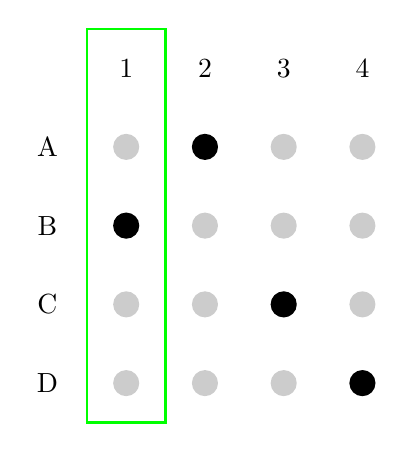
\begin{tikzpicture}
        
		\foreach \x / \y in {1/A,2/B,3/C,4/D} {
		\node (0-\x) at (0, -\x) {\y};
		\node (\x-0) at (\x, 0) {\x};
		}
        
		\foreach \x in {1,...,4} {
		\foreach \y in {1,...,4} 
		\node[circle, fill=black!20] (\x-\y) at (\x, -\y) {};
		}

		\foreach \x / \y in {1/2, 2/1, 3/3, 4/4} {
		\node[circle, fill=black] at (\x,-\y) {};
		}
        
		\draw[green, thick] (0.5,0.5) rectangle (1.5,-4.5);
        
	\end{tikzpicture}}
	\qquad
	\subfigure{
	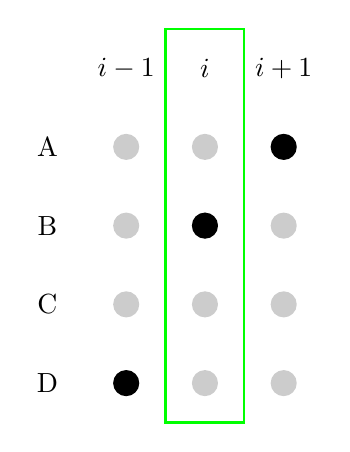
\begin{tikzpicture}
		\foreach \x / \y in {1/A,2/B,3/C,4/D}
		\node (0-\x) at (0, -\x) {\y};
        
		\foreach \x / \y in {1/$i-1$, 2/$i$, 3/$i+1$}
		\node (\x-0) at (\x, 0) {\y};
        
		\foreach \x in {1,...,3}
		\foreach \y in {1,...,4} 
		\node[circle, fill=black!20] at (\x, -\y) {}; 
                
		\foreach \x / \y in {4/1, 2/2, 1/3} {
		\node[circle, fill=black] at (\y,-\x) {};
        
		\draw[green, thick] (1.5,0.5) rectangle (2.5,-4.5);
		}
	\end{tikzpicture}}
	\caption{Interpretazione grafica di $E_1$}
\end{figure}


\newpage


Di seguito si riportano i vincoli per il TSP:

\begin{enumerate}
	\item \textbf{Vincolo sulle righe}: Ogni città deve essere visitata una sola volta. Ovvero le righe della matrice $V$ devono avere soltanto un elemento impostato ad 1, il resto a 0;
	\begin{align*}
		E_2 = \frac{A}{2} \sum_X \sum_i \sum_{j \neq i} V_{X,i} V_{X,j}
	\end{align*}
	che vale 0 (il minimo) se ogni città è visitata al massimo una volta.
	\item \textbf{Vincolo sulle colonne}: Ogni fermata deve contenere una città, ovvero ogni colonna della matrice $V$ abbia un elemento impostato ad 1 ed il resto a 0;
	\begin{align*}
		E_3 = \frac{B}{2} \sum_i \sum_X \sum_{Y \neq X} V_{X,i} V_{Y,i}
	\end{align*}
	che vale 0 se ogni step del tour contiene al massimo una città.
	\item \textbf{Vincolo sulle entrate}: in totale devono essere attraversate $n$ città.
	\begin{align*}
		E_4 = \frac{C}{2}\left(\sum_X \sum_i V_{X,i} - n \right)^2
	\end{align*}
	che vale 0 se il numero di città attraversate è esattamente $n$.
\end{enumerate}

Ci si trova dunque con quattro funzioni energia da minimizzare, tuttavia per poter utilizzare una rete di Hopfield è necessaria un'unica funzione. Per questo motivo si esprime la funzione costo totale come combinazione lineare delle funzioni energia $E_i$:
\begin{align}
	E = E_1 + E_2 + E_3 + E_4
\end{align}
dove il peso da attribuire a ciascun termine è determinato dalle costanti positive $A, B, C, D$. La funzione energia risultante dovrà essere della forma tipica di una rete di Hopfield ovvero nella forma dell'Equazione~\eqref{eq:energy}:
\begin{align*}
	E = - \frac{1}{2} \sum_{X, Y} \sum_{i, j} T_{X_i, Y_j} V_{X_i} V_{Y_j} - \sum_{X_i} I_{X_i} V_{X_i}
\end{align*}

\newpage

Per ricondursi alla funzione energia tipica di Hopfield si utilizza un “trucco”: si introduce il seguente termine:
\begin{align*}
	\delta_{i,j} =
	\begin{cases}
		1, &\text{ se } i = j\\
		0, &\text{ se } i \neq j \\
	\end{cases}
\end{align*}
Le funzioni energia si possono ora riscrivere nel seguente modo:
\begin{align*}
	E_1 &= \frac{D}{2} \sum_X \sum_{Y \neq X} \sum_i d_{X,Y} V_{X,i} (V_{Y, i+1} + V_{Y, i-1}) \\
	&=  \frac{D}{2} \sum_{X,Y} \sum_{i,j} d_{X,Y} V_{X,i} V_{Y,j} \cdot (\delta_{j, i-1} + \delta_{j, i+1})
\end{align*}

\begin{align*}
	E_2 &= \frac{A}{2} \sum_X \sum_i \sum_{j \neq i} V_{X,i} V_{X,j} \\
	&= \frac{A}{2} \sum_{X,Y} \sum_{i,j} V_{X,i} V_{Y,j} \delta_{X,Y} (1 - \delta_{i,j})
\end{align*}

\begin{align*}
	E_3 &= \frac{B}{2} \sum_i \sum_X \sum_{Y \neq X} V_{X,i} V_{Y,i} \\
	&= \frac{B}{2} \sum_{X,Y} \sum_{i,j} V_{X,i} V_{Y,j} \delta_{i,j} (1 - \delta_{X,Y})
\end{align*}

\begin{align*}
	E_4 &= \frac{C}{2}\left(\sum_X \sum_i V_{X,i} - n \right)^2 \\
	&= \frac{C}{2} \left(\left(\sum_X \sum_i V_{X,i}\right)^2 - 2n \cdot \sum_X \sum_i V_{X,i} + n^2 \right)
\end{align*}
dove
\begin{align*}
	\left(\sum_X \sum_i V_{X,i}\right)^2 &= \left(\sum_X \sum_i V_{X,i}\right) \cdot \left(\sum_X \sum_i V_{X,i} \right) \\
	&= \sum_{X,Y} \sum_{i,j} V_{X,i} V_{Y,j}
\end{align*}

\newpage

In $E_4$ il termine costante $n^2$ si può tralasciare, in quanto non modifica il punto in cui si ottiene il minimo, ma il valore della funzione $E_4$ in corrispondenza del minimo.
Mettendo il tutto assieme si ottiene la \textbf{funzione di energia totale}:
\begin{align*}
	E &= \frac{A}{2} \sum_{X,Y} \sum_{i,j} V_{X,i} V_{Y,j} \delta_{X,Y} (1 - \delta_{i,j}) \\
	&+ \frac{B}{2} \sum_{X,Y} \sum_{i,j} V_{X,i} V_{Y,j} \delta_{i,j} (1 - \delta_{X,Y}) \\
	&+ \frac{C}{2} \left(\sum_{X,Y} \sum_{i,j} V_{X,i} V_{Y,j} - \sum_{X,i} V_{X,i} \right) \\
	&+ \frac{D}{2} \sum_{X,Y} \sum_{i,j} d_{X,Y} V_{X,i} V_{Y,j} \cdot (\delta_{j, i-1} + \delta_{j, i+1}) \\
	&= - \frac{1}{2} \sum_{X, Y} \sum_{i, j} T_{X_i, Y_j} V_{X_i} V_{Y_j} - \sum_{X_i} I_{X_i} V_{X_i}
\end{align*}
Dove $T_{Xi, Yj}$ sono i pesi che la rete deve scoprire:
\begin{align*}
	T_{Xi, Yj} &= - A \delta_{XY} (1 - \delta_{ij}) \tag{peso inibitorio in ogni riga}\\
	& - B \delta_{ij} (1 - \delta_{XY}) \tag{peso inibitorio in ogni colonna} \\
	& - C  \qquad \tag{Inibizione globale}\\
	& - D d_{XY} (\delta_{j,i-1} + \delta_{j, i+1}) \tag{Termine dei dati}
\end{align*}
e il vettore di corrente esterna $I$ ha come $Xi$-esima componente:
\begin{align*}
	I_{Xi} = C_n \tag{Corrente esterna eccitatoria}
\end{align*}
% subsection soluzione_del_tsp_con_le_reti_di_hopfield (end)

\newpage

\subsection{Un'altra formulazione} % (fold)
\label{sub:un_altra_formulazione}
La determinazione dei parametri $A, B, C, D$ è particolarmente difficile. Pertanto un altro modo per esprimere i vincoli del TSP (cioè la matrice di permutazione $V$) è il seguente:
\begin{align*}
	E_2 = \frac{A}{2} \sum_X \left(\sum_i V_{X, i} - 1 \right) ^ 2 \tag{Vincolo sulle righe} \\
	E_3 = \frac{B}{2} \sum_i \left(\sum_X V_{X, i} - 1 \right) ^ 2 \tag{Vincolo sulle colonne} \\
\end{align*}
Quindi la funzione energia diventa:
\begin{align*}
	E = \frac{D}{2} \sum_{X} \sum_{Y \neq X} \sum_i d_{X,Y} V_{X,i}(V_{Y, i + 1} + V_{Y, i - 1}) + E_2 + E_3
\end{align*}
Dal momento che $E_4$ non è usato abbiamo tre parametri anziché quattro.
% subsection un_altra_formulazione (end)


\subsection{Problema delle n regine} % (fold)
\label{sub:problema_delle_n_regine}
Una famosa variante del TSP è il \emph{problema delle n regine}. Si immagini una scacchiera $n \times n$ e $n$ regine; una regina può muoversi lungo le righe, le colonne e le diagonali. Il problema consiste nel posizionare questi $n$ pezzi in modo tale che nessuno di essi possa attaccarsi l'uno contro l'altro.\\

Si può costruire una rete di Hopfield $n \times n$ in cui il neurone $(i,j)$ è attivo se e solo se una regina occupa la posizione $(i,j)$. Ci sono inoltre quattro vincoli:
\begin{enumerate}
	\item solo una regina in ciascuna riga;
	\item solo una regina in ciascuna colonna;
	\item solo una regina in ciascuna diagonale;
	\item solo $n$ regine sulla scacchiera.
\end{enumerate}


\newpage

Il problema è analogo al TSP con l'aggiunta del vincolo sulle diagonali. La matrice dei pesi è quindi data da:
\begin{align*}
	- T_{ij,kl} &= - A \delta_{ik} (1 - \delta_{ij}) \tag{peso inibitorio in ogni riga}\\
	& + B \delta_{jl} (1 - \delta_{ik}) \tag{peso inibitorio in ogni colonna} \\
	& + C  \qquad \tag{Inibizione globale}\\
	& + D (\delta_{i+j,k-l} + \delta_{i-j, k-l})(1 - \delta_{ik}) \tag{peso inibitorio sulle diagonale}
\end{align*}

L'ottimizzazione tramite le reti di Hopfield presenta, tuttavia, alcuni svantaggi:
\begin{enumerate}
	\item sono necessari $n^2$ neuroni;
	\item il numero di connessioni è e $O(n^4)$;
	\item i parametri $A, B, C, D$ sono difficili da determinare;
	\item i risultati ottenuti sono raramente soluzioni ammisibili, ovvero matrici binarie con i vincoli rispettati;
	\item è difficile evitare il problema dei minimi locali.
\end{enumerate}

% subsection problema_delle_n_regine (end)
% section problema_del_commesso_viaggiatore (end)

\newpage

\section{Problema della cricca massima} % (fold)
\label{sec:problema_della_cricca_massima}

Sia $G=(V,E)$ un grafo non orientato con $V$ l'insieme dei vertici ed $E$ quello degli archi, tale per cui $V={1,\dots,n}$ e $E \subseteq V \times V$. Si definisce cricca (o clique) $C \subseteq V$, un sottoinsieme di vertici di G mutuamente adiacenti (che formano un grafo completo), ovvero tali che $\forall i,j \in C$ con $i \neq j, (i,j) \in E$.

\begin{mydef}[Clique massimale]
	Si definisce \textbf{clique massimale} di $G$ una clique di $G$ che non è contenuta in nessun'altra clique di $G$.    
\end{mydef}

\begin{mydef}[Clique massima]
	Si definisce \textbf{clique massima} di $G$ una clique massimale di G di cardinalità massima.
\end{mydef}
Il problema consiste nel trovare una cricca massimale (MCP). Ad esempio si consideri il seguente grafo:

\begin{figure}[h!]
	\centering
	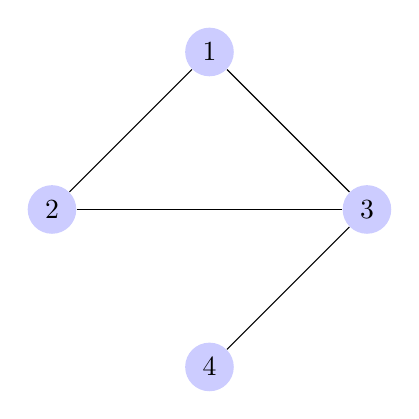
\begin{tikzpicture}
		\node[circle,fill=blue!20] (1) at (0,2) {1};
		\node[circle,fill=blue!20] (2) at (-2,0) {2};
		\node[circle,fill=blue!20] (3) at (2,0) {3};
		\node[circle,fill=blue!20] (4) at (0, -2) {4};
    
		\foreach \from / \to in {1/2,2/3,1/3,3/4}
		\path (\from) edge (\to);
	\end{tikzpicture}
	\caption{Un grafo non orientato.}\label{fig:graph1}
\end{figure}
Alcune clique nel grafo sono:
\begin{align*}
	C_1 &= \{1,2\} \tag{$C_1$ non è massimale perché $C_1 \subseteq C_2$}\\
	C_2 &= \{1,2,3\} \tag{Massimale e massima}\\
	C_3 &= \{3,4\} \tag{Massimale}
\end{align*}

\newpage

Trovare una clique massimale è un problema facile, mentre trovare quella massima è NP-difficile, così come trovare la dimensione di tale clique. In questa sezione si affronta il problema sotto quest'ultimo punto di vista.

\subsection{Formulazione continua di MCP} % (fold)
Per affrontare il problema con le reti neurali è necessario trasformare MCP da problema discreto a problema continuo. Nell'esempio del TSP con il modello di Hopfield, non è detto che ci sia il percorso inverso (potremo ottenere ad esempio una matrice che non ha significato); in questo nuovo problema MCP, la bidirezionalità è d'obbligo.\\

Si utilizza quindi un nuovo approccio, ma prima sono necessarie alcune notazioni:
\begin{itemize}
	\item Se $C \subseteq V$, $x^C$ indica il \textbf{vettore caratteristico} definito come:
	\begin{align*}
		x^C_i = 
		\begin{cases}
			\displaystyle\frac{1}{|C|}, &\text{se }i \in C\\
			0,  &\text {altrimenti}
		\end{cases}
	\end{align*}
	dove $|C|$ indica la cardinalità dell'insieme $C$ e $i \in \{ 1, \dots, |V|\}$
	\item $S_n$ è il \textbf{simplesso standard} in $\mathbb{R}^n$:
	\begin{align*}
		S_n = \left\{x \in \mathbb{R}^n : \sum_{i=1}^n x_i = 1 \text{ e } x_i \geq 0, \forall i \right\}
	\end{align*}
	Per qualunque vettore caratteristico vale la relazione $x^C \in S_n$ con $n \geq |C|$
	\item $A=(a_{ij})$ è la matrice di adiacenza di $G$:
	\begin{align*}
		a_{ij} =
		\begin{cases}
			1, &\text{ se } (i,j) \in E \\
			0, &\text{ altrimenti}
		\end{cases}
	\end{align*}
\end{itemize}

\newpage

\begin{figure}[h!]
	\centering
	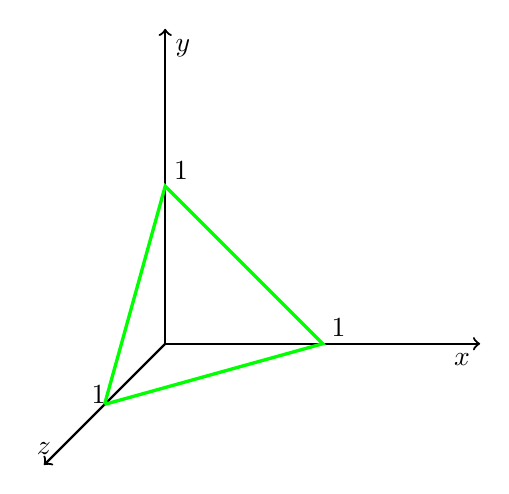
\begin{tikzpicture}[scale=2]

		%draw the main coordinate system axes
		\draw[thick,->] (0,0,0) -- (2,0,0) node[anchor=north east]{$x$};
		\draw[thick,->] (0,0,0) -- (0,2,0) node[anchor=north west]{$y$};
		\draw[thick,->] (0,0,0) -- (0,0,2) node[anchor=south]{$z$};
        
		\draw[thick, color=green, very thick] plot coordinates{(0,0,1) (0,1,0) (1,0,0) (0,0,1)};
        
		\node at (1.1,0.1,0) {1};
		\node at (0.1,1.1,0) {1};
		\node at (0,0.1,1.1) {1};
        
	\end{tikzpicture}
	\caption{Rappresentazione grafica del simplesso standard}
\end{figure}

Si consideri la seguente funzione quadratica continua in $n$ variabili:
\begin{align*}
	&f_G(x) = x^T A x = \sum_{i=1}^n \sum_{j=1}^n a_{ij} x_i x_j \tag{Lagrangiano del grafo} \\
	&\text{oppure } f_G(\bar{x}) = \sum_{(i,j) \in E} x_i x_j
\end{align*}
dove $x^T$ è il vettore trasposto e $A$ è la matrice di adiacenza. Ad esempio se si considera il grafo in Figura~\ref{fig:graph1} allora:
\begin{align*}
	f_G(x) = x_1 x_2 + x_1 x_3 + x_2 x_3 + x_3 x_4
\end{align*}

È stata dunque definita una funzione continua che rappresenta il problema: il Lagrangiano del grafo. A questo punto l'approccio tipico per risolvere MCP è quello di costruire un sistema dinamico che converga ai massimi di tale funzione. Questi punti corrisponderanno alle soluzioni nello spazio discreto del problema originale. A tale scopo si introduce il teorema di Motzkin-Strauss.
\begin{thm}[Teorema di Motzkin-Strauss]
	Sia $x^*$ un massimo globale di $f_G$ in $x \in S_n$ allora la cardinalità della clique massima è legata a $f_G(x)$  dalla seguente formula:
	\begin{align*}
		\omega(G) = \frac{1}{1 - f(x^*)}
	\end{align*}
	Inoltre un sottoinsieme di vertici $C$ è una clique massima se e solo se il suo vettore caratteristico $x^C \in S_n$ è un massimo globale per $f_G$ in $S_n$.
	\end{thm} 
	\newpage

	Il teorema di Motzkin-Strauss fornisce una connessione tra la cardinalità della clique massima $\omega(G)$ di un grafo $G$ con $n$ vertici e il massimo del suo Lagrangiano definito nel simplesso standard di $\mathbb{R}^n$. In particolare è stato mostrato che una clique $C$ è massima se e solo se il suo vettore caratteristico $x^C$ è un massimizzatore globale della funzione $f_G$ su $S_n$.\\

	Tuttavia non tutti i massimizzatori di $f_G$ sono nella forma di vettori caratteristici e pertanto non possono essere utilizzati direttamente per ricavare informazioni sulle clique massime. Tali massimizzatori sono definiti \emph{soluzioni spurie}. Ad esempio, si consideri il seguente grafo:

	\begin{figure}[h!]
		\centering
		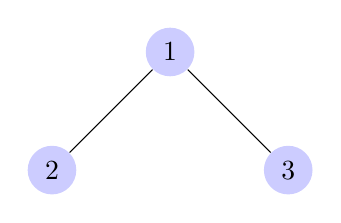
\begin{tikzpicture}
			\node[circle,fill=blue!20] (1) at (0,1.5) {1};
			\node[circle,fill=blue!20] (2) at (-1.5,0) {2};
			\node[circle,fill=blue!20] (3) at (1.5,0) {3};
        
			\draw (1) -- (2);
			\draw (1) -- (3);
        
		\end{tikzpicture}
		\caption{Grafo esempio.}
	\end{figure}
	Il grafo presenta due massimi globali:
	\begin{align*}
		C_1 = \{1,2\} \qquad  x^{C_1} = (1 / 2, 1 / 2, 0) \\
		C_2 = \{1,3 \} \qquad x^{C_2} = (1 / 2, 0, 1 / 2)
	\end{align*}

	Tuttavia come si evince dal seguente grafico, sono massimi globali anche tutti i punti del segmento $x'x''$ ovvero tutti i punti in $(1/2, \alpha / 2, (1 - \alpha) / 2) \, \forall \alpha \in [0,1]$.
	\begin{figure}[h!]
		\centering
		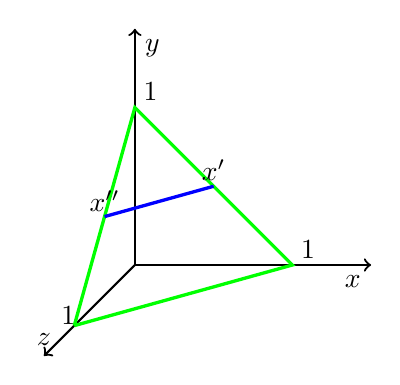
\begin{tikzpicture}[scale=2]
			%draw the main coordinate system axes
			\draw[thick,->] (0,0,0) -- (1.5,0,0) node[anchor=north east]{$x$};
			\draw[thick,->] (0,0,0) -- (0,1.5,0) node[anchor=north west]{$y$};
			\draw[thick,->] (0,0,0) -- (0,0,1.5) node[anchor=south]{$z$};
        
			\draw[thick, color=green, very thick] plot coordinates{(0,0,1) (0,1,0) (1,0,0) (0,0,1)};
			\draw[color=blue, very thick] (.5, .5, 0) -- (0,.5,.5);
        
			\node at (.5,.6,0) {$x'$};
			\node at (0,.6,.5) {$x''$};
        
			\node at (1.1,0.1,0) {1};
			\node at (0.1,1.1,0) {1};
			\node at (0,0.1,1.1) {1};
        
		\end{tikzpicture}
		\caption{Soluzioni spurie in MCP}
	\end{figure}

	Dunque $x'$ e $x''$ \textbf{non} sono vettori caratteristici e non possono essere utilizzati per la soluzione del MCP.

	\newpage

	Quello che è stato fatto finora è prendere il problema $P$ di clique massima nel discreto e trasformarlo in un problema $P'$ di ottimizzazione quadratica nel continuo. A questo punto è necessario mappare la soluzione del problema $P'$ in una soluzione del problema originale $P$.  Questo è possibile se la soluzione ottenuta in $P'$ è un vettore caratteristico.\\

	Il problema delle soluzioni spurie è stato risolto da Immanuel Bomze (1995) proponendo una versione regolarizzata di $f_G(x)$. La soluzione consiste nel sommare $1/2$ alla diagonale principale della matrice di adiacenza $A$.
	\begin{align*}
		A' = A + \frac{1}{2} I
	\end{align*}
	Da cui si ottiene:
	\begin{align*}
		\hat{f}_G(x) = x^T A' x = x^T \left( A + \frac{1}{2} I \right) x 
	\end{align*}
	Dove I è la matrice identità, ovvero una matrice quadrata dello stesso lato di $A$ con tutti gli elementi in diagonale principale ad 1 e tutti gli elementi al di fuori di essa a 0.\\


	\begin{figure}[h!]
		\centering
		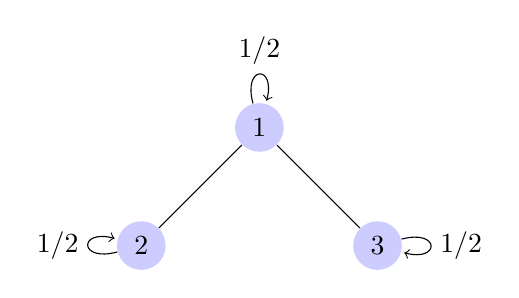
\begin{tikzpicture}
			\node[circle,fill=blue!20] (1) at (0,1.5) {1};
			\node[circle,fill=blue!20] (2) at (-1.5,0) {2};
			\node[circle,fill=blue!20] (3) at (1.5,0) {3};
        
			\path
			(1) edge (2)
			(1) edge (3)
			(1) edge[loop above] node{$1/2$} (1)
			(2) edge[loop left] node{$1/2$} (2)
			(3) edge[loop right] node{$1/2$} (3)
			;
		\end{tikzpicture}
		\caption{Soluzione problema delle soluzioni spurie (Bomze).}
	\end{figure}

	Riassumendo il problema della cricca massima dato un grafo $G = (V, E)$ è definito nel seguente modo:
	\begin{align*}
		\max(\hat{f}_G(x)) \text{ tale che } x \in S_n
	\end{align*}
	Sia $C \subseteq V$ e sia $x^C$ il suo vettore caratteristico allora:
	\begin{enumerate}
		\item $C$ è una clique massima di $G$ sse $x^C$ è un massimo globale di $\hat{f} \in S_n$;
		\item $C$ è una clique massimale di $G$ sse $x^C$ è un massimo locale di $\hat{f} \in S_n$;
		\item ogni massimo locale è un vettore caratteristico ed è locale stretto. 
	\end{enumerate}

	\newpage

	Il risultato precedente garantisce che \emph{tutti} i massimizzatori di $\hat{f}$ su $S_n$ sono stretti, e sono sono vettori caratteristici di clique massima/massimale in un grafo. In particolare esiste una corrispondenza uno-a-uno da una parte tra le clique massimali e massimizzatori locali di $\hat{f}$ su $S_n$, dall'altra tra clique massima e massimizzatore globale.

	% section problema_della_cricca_massima (end)


	% chapter ottimizzazione_con_le_reti_neurali (end)

	% part reti_neurali (end)
    
	\part{Teoria dei Giochi} % (fold)
	\label{prt:teoria_dei_giochi}
	%!TEX root = ../main.tex

\chapter{Teoria dei giochi}
\label{cha:teoria_dei_giochi}

La \textbf{teoria dei giochi} analizza situazioni in cui vi sono interazioni tra \textbf{agenti} diversi, ove ognuno è interessato a \textbf{massimizzare} il proprio \textbf{beneficio}, tali per cui le scelte di un agente possono influire sul beneficio che possono ottenere gli altri agenti. Essa è stata sviluppata con il preciso scopo di sopperire alle limitazioni legate all'ottimizzazione di una \textbf{singola} funzione obiettivo.

Vediamo brevemente gli avvenimenti più importanti nello studio della teoria dei giochi:
\begin{itemize}
	\item \textbf{1921 - 1928}: prima formulazione di strategia mista e l'idea di trovare soluzioni di giochi in forma normale (E. Borel, J. von Neumann);
	\item \textbf{1944, 1947}: pubblicazione di 	\emph{Theory of Games and Economic Behavior} (J. von Neumann, O. Morgenstern);
	\item \textbf{1950 - 1953}: contributi alla teoria dei giochi non cooperativi (J. Nash);
	\item \textbf{1972 - 1982}: applicazione della teoria dei giochi a problemi biologici (J. M. Smith).
\end{itemize}

\section{Giochi finiti in forma normale}
\label{sec:giochi_finiti_in_forma_normale}

Un gioco finito in forma normale consiste di un insieme di \textbf{giocatori}
\begin{displaymath}
	I = \{1, \dots, n\} \qquad (n \geq 2)
\end{displaymath}
ciascuno dei quali ha a disposizione un insieme di \textbf{azioni} (dette anche \textbf{strategie pure}):
\begin{displaymath}
	S_i = \{1, \dots, m_i\} \qquad (m_i \geq 2)
\end{displaymath}
L'insieme delle azioni giocate dagli individui in un dato istante prende il nome di \textbf{profilo strategico puro}
\begin{displaymath}
	\vec{s} = (s_1, \dots, s_n)
\end{displaymath}
e l'insieme dei profili strategici puri forma lo \textbf{spazio delle strategie pure}:
\begin{displaymath}
	S = \prod_{i = 1}^n S_i
\end{displaymath}
In seguito alla giocata di un profilo strategico $\vec{s} \in S$ ciascun individuo $i \in I$ ottiene un \textbf{payoff}, ovvero la quantificazione del beneficio ottenuto dal giocatore in seguito alla giocata. Il payoff del giocatore $i$ è rappresentato dalla funzione $\pi_i: S \rightarrow \mathbb{R}$; la \textbf{funzione di payoff combinata} $\vec{\pi}: S \rightarrow \mathbb{R}^n$ assegna ad ogni profilo strategico $\vec{s} \in S$ il vettore
\begin{displaymath}
	\vec{\pi}(\vec{s}) = (\pi_1(\vec{s}), \dots, \pi_n(\vec{s}))
\end{displaymath}
Un gioco in forma normale può dunque essere rappresentato dalla tripletta $(I, S, \vec{\pi})$.

\section{Giochi a due giocatori}

Nel caso speciale di giochi a due giocatori, è comodo rappresentare le funzioni di payoff in forma matriciale:
\begin{itemize}
	\item $\mat{A} = (a_{ij})$ è la matrice di payoff del primo giocatore, dove $a_{ij} = \pi_1(i, j)$ con $i \in S_1, j \in S_2$;
	\item $\mat{B} = (b_{ij})$ è la matrice di payoff del secondo giocatore, dove $b_{ij} = \pi_2(i, j)$ con $i \in S_1, j \in S_2$;
\end{itemize}
In base alle caratteristiche di $\mat{A}$ e $\mat{B}$ si possono distinguere delle categorie particolari di giochi:
\begin{itemize}
	\item \textbf{giochi a somma zero}: $\mat{A} + \mat{B} = \mat{0}$;
	\item \textbf{giochi simmetrici}: $\mat{A} = \mat{B}^T$;
	\item \textbf{giochi doppiamente simmetrici}: $\mat{A} = \mat{A}^T = \mat{B}^T$.
\end{itemize}

\section{Giochi succinti}

Per descrivere un gioco in forma normale, con $n$ giocatori e $m$ strategie pure per ciascuno, occorre memorizzare $n m^n$ numeri. Un \textbf{gioco succinto} è un gioco rappresentabile in forma molto più ridotta rispetto alla forma normale; ad esempio:
\begin{itemize}
	\item \textbf{giochi sparsi}, dove la maggior parte dei payoff è $0$;
	\item \textbf{giochi grafici}, dove i payoff di un giocatore dipendono dalle scelte di $d < n$ giocatori;
	\item \textbf{giochi simmetrici}.
\end{itemize}

\section{Polymatrix games}

Un \textbf{polymatrix game} è un gioco non cooperativo\footnote{Un gioco si dice \textbf{non cooperativo} se non c'è collaborazione tra i giocatori: tutti i giochi che tratteremo sono di questo tipo.} succinto in cui l'influenza relativa della scelta di una strategia da parte di un giocatore sul payoff di un altro è sempre la stessa, indipendentemente da cosa faranno i rimanenti giocatori. Formalmente:
\begin{itemize}
	\item ci sono $n$ giocatori con $m$ strategie pure ciascuno;
	\item c'è una matrice di payoff $A^{ij} = (a_{kl}^{ij})$ di dimensione $m \times m$ per ogni coppia di giocatori $(i, j)$;
	\item il payoff del giocatore $i$ per il profilo strategico puro $\vec{s}$ è:
	\begin{displaymath}
		u_i(\vec{s}) = \sum_{j \neq i} a_{s_i s_j}^{ij}
	\end{displaymath}
\end{itemize}
Il numero di payoff da memorizzare è $\mathcal{O}(m^2 n^2)$. Il problema di trovare un equilibrio di Nash in un gioco di questo tipo è PPAD-completo.\footnote{PPAD è un sottoinsieme di TFNP, un'estensione della classe di problemi decisionali NP a relazioni totali. Una relazione binaria $P \in TFNP$ se e solo se esiste un algoritmo che può verificare in tempo polinomiale se, dati $x$ e $y$, $P(x, y)$ è verificata e $\forall x \exists y$ tale che $P(x, y)$ vale.}

\section{Strategie miste}

Supponiamo che il giocatore $i \in I$ decida la strategia pura da usare in base ad una distribuzione di probabilità sull'insieme di strategie pure $S_i$: tale distribuzione prende il nome di \textbf{strategia mista}. Essa può essere rappresentata da un vettore $m_i$-dimensionale $\vec{x}_i$ dove $x_{ih}$ è la probabilità che il giocatore $i$ giochi la sua strategia pura $h$. Per definizione di distribuzione di probabilità, $\vec{x}_i$ appartiene al simplesso standard $m_i$-dimensionale $\Delta_i$:
\begin{displaymath}
	\Delta_i = \left\{ \vec{x}_i \in \R^{m_i} : \sum_{h = 1}^{m_i} x_{ih} = 1 \text{ e } x_{ih} \geq 0 \; \forall h \right\}
\end{displaymath}
L'insieme delle strategie pure cui è assegnata una probabilità positiva prende il nome di \textbf{supporto} di $\vec{x_i}$:
\begin{displaymath}
	\sigma(\vec{x_i}) = \{h \in S_i : x_{ih} > 0 \}
\end{displaymath}
Una strategia pura $h$ può essere vista come una \textbf{strategia mista estrema} $\vec{x}_i$ dove $x_{ih} = 1$ e $x_{ij} = 0$ per $j \neq h$. Ogni strategia mista può essere espressa come combinazione lineare di strategie miste estreme.

\begin{figure}[h!]
	\centering
	\subfigure[]{
	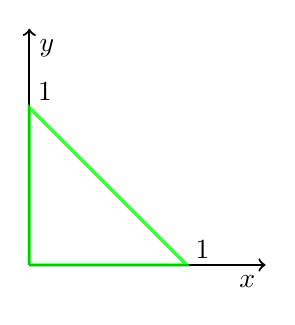
\begin{tikzpicture}[scale=2]
        %draw the main coordinate system axes
        \draw[thick,->] (0,0) -- (1.5,0) node[anchor=north east]{$x$};
        \draw[thick,->] (0,0) -- (0,1.5) node[anchor=north west]{$y$};
        
        \draw[thick, opacity=0.8, color=green, very thick] plot coordinates{(0,0) (0,1) (1,0) (0,0)};
    
        \node at (1.1,0.1) {1};
        \node at (0.1,1.1) {1};
    \end{tikzpicture}}
	\qquad\qquad
	\subfigure[]{
	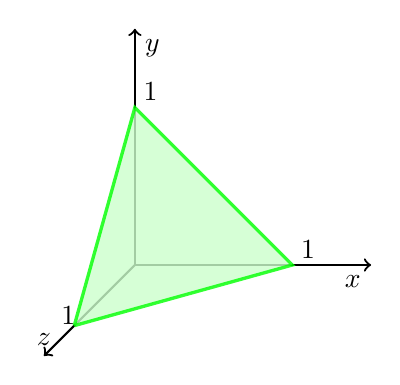
\begin{tikzpicture}[scale=2]
        %draw the main coordinate system axes
        \draw[thick,->] (0,0,0) -- (1.5,0,0) node[anchor=north east]{$x$};
        \draw[thick,->] (0,0,0) -- (0,1.5,0) node[anchor=north west]{$y$};
        \draw[thick,->] (0,0,0) -- (0,0,1.5) node[anchor=south]{$z$};
    
        \filldraw[thick, opacity=0.8, color=green!20, draw=green, very thick] plot coordinates{(0,0,1) (0,1,0) (1,0,0) (0,0,1)};
    
        \node at (1.1,0.1,0) {1};
        \node at (0.1,1.1,0) {1};
        \node at (0,0.1,1.1) {1};
	\end{tikzpicture}}
	\caption[Simplesso 2D e 3D]{A sinistra il simplesso a due dimensioni, a destra quello a tre dimensioni. Le strategie pure corrispondono ai vertici del simplesso.}
\end{figure}

\noindent Un \textbf{profilo strategico misto} è un vettore $\vec{x} = (\vec{x}_1, \dots, \vec{x}_n)$ dove la componente $\vec{x}_i$ è una strategia mista del giocatore $i \in I$. Lo \textbf{spazio delle strategie miste} è il multi-simplesso $\Theta = \prod_{i = 1}^n \Delta_i$.

Nei giochi non cooperativi si assume che le scelte dei giocatori siano indipendenti tra loro, pertanto la probabilità che un profilo strategico puro $\vec{s}$ sia usato quando viene giocato un profilo strategico misto $\vec{x}$ è data da
\begin{displaymath}
    \mathbf{\vec{x}(\vec{s})} = \prod_{i = 1}^n x_{i s_i}
\end{displaymath}
e il \textbf{payoff atteso} del giocatore $i \in I$ è
\begin{displaymath}
    u_i(\vec{x}) = \sum_{\vec{s} \in S} \vec{x}(\vec{s}) \pi_i(\vec{s})
\end{displaymath}

\section{Best replies ed equilibri di Nash}

\begin{mydef}[Best reply]
	La \defterm{best reply} di un giocatore $i \in I$ al profilo strategico $\vec{x}_{-i}$\footnote{Con $\vec{x}_{-i}$ si intende il profilo strategico misto $\vec{x} \in \Theta$ senza la componente $i$-esima.} è una strategia mista $\vec{x}_i^* \in \Delta_i$ tale per cui:
	\begin{displaymath}
		u_i(\vec{x}_i^*, \vec{x}_{-i}) \geq u_i(\vec{z}_i, \vec{x}_{-i}) \quad \forall \vec{z}_i \in \Delta_i
	\end{displaymath}
\end{mydef}
\noindent L'\textbf{insieme delle best replies} a una strategia $\vec{x}_{-i}$ per $i \in I$ si indica con $\beta_i^*(\vec{x}_{-i})$. Si noti che, escluso il caso in cui c'è un'unica miglior risposta (che è una strategia pura), il numero di best replies è infinito. Infatti:
\begin{itemize}
	\item quando il supporto di una best reply include due o più strategie pure, una loro combinazione è una best reply;
	\item se due strategie pure sono individualmente best replies, una loro combinazione è una best reply.
\end{itemize}
Il concetto di equilibrio di Nash è motivato dall'idea che una teoria di decision-making razionale non dovrebbe creare un incentivo a deviare da essa per coloro i quali ci credono.
\begin{mydef}[Equilibrio di Nash]
	Un profilo strategico $\vec{x} \in \Theta$ è un \defterm{equilibrio di Nash} se è una best reply a sè stesso, ovvero:
	\begin{displaymath}
		u_i(\vec{x}_i, \vec{x}_{-i}) \geq u_i(\vec{z}_i, \vec{x}_{-i}) \quad \forall \vec{z}_i \in \Delta_i, \forall i \in I
	\end{displaymath}
	Un equilibrio di Nash si dice \defterm{stretto} se la disuguaglianza è stretta per $\vec{z}_i \neq \vec{x}_i$.
\end{mydef}
\begin{thm}
	Un profilo strategico $\vec{x} \in \Theta$ è un equilibrio di Nash se e solo se, per ogni giocatore $i \in I$, ogni strategia pura nel supporto di $\vec{x}_i$ è una best reply a $\vec{x}_{-i}$.
\end{thm}
\noindent L'esistenza di un equilibrio di Nash è garantita dal seguente teorema.
\begin{thm}[J. Nash, 1951]
	Ogni gioco finito in forma normale ammette un equilibrio di Nash misto.
\end{thm}

\section{Teoria dei giochi evolutivi}

La \textbf{teoria dei giochi evolutivi} è una disciplina introdotta da J. M. Smith per modellare l'evoluzione del comportamento animale utilizzando mezzi e principi della teoria dei giochi. Si basa sulle seguenti assunzioni:
\begin{itemize}
	\item una popolazione grande (idealmente infinita) di individui appartenenti alla stessa specie competono per risorse disponibili in \textbf{quantità limitata};
	\item il conflitto è modellato come un gioco \textbf{simmetrico a due giocatori} selezionati in maniera casuale tra la popolazione;
	\item gli individui non giocano razionalmente, ma seguono un \textbf{pattern preprogrammato};
	\item la riproduzione è \textbf{asessuata} per cui, a meno di mutazioni, ogni nascituro sarà un clone del genitore, ovvero programmato alla sua stessa strategia;
	\item il payoff è espresso in termini di \textbf{successo riproduttivo}.
\end{itemize}
In questo framework, una strategia mista può essere interpretata in due modi matematicamente equivalenti:
\begin{itemize}
	\item ogni individuo gioca una strategia pura, ma parte della popolazione segue una strategia, il resto ne segue altre;
	\item ogni individuo gioca la stessa strategia mista.
\end{itemize}
Per trattare aspetti dinamici, la prima formulazione è la più conveniente.

\section{Strategie evolutivamente stabili}

Assumiamo che un piccolo gruppo di \textbf{invasori}, che segue una strategia $\vec{y} \in \Delta$, appaia in una popolazione che segue la strategia $\vec{x} \in \Delta$; sia $\epsilon \in (0, 1)$ la percentuale di invasori nella popolazione complessiva.

Il \textbf{payoff} in un gioco di questo tipo è lo stesso che si otterrebbe in un gioco con individui che seguono la strategia $\epsilon \vec{y} + (1 - \epsilon) \vec{x} \in \Delta$.
\begin{mydef}[Strategie evolutivamente stabili (ESS)]
	Una strategia $\vec{x} \in \Delta$ si dice \defterm{evolutivamente stabile} se per ogni $\vec{y} \in \Delta \setminus \{\vec{x}\}$ esiste $\delta \in (0, 1)$ tale per cui, per ogni $\epsilon \in (0, \delta)$, si ha
	\begin{displaymath}
		\underbrace{u(\vec{x}, \epsilon \vec{y} + (1 - \epsilon) \vec{x})}_{\text{strategia \textbf{attuale}}} > \underbrace{u(\vec{y}, \epsilon \vec{y} + (1 - \epsilon) \vec{x})}_{\text{strategia \textbf{mutante}}}
	\end{displaymath}
\end{mydef}
\begin{thm}
	Una strategia $\vec{x} \in \Delta$ è evolutivamente stabile se e solo se:
	\begin{itemize}
		\item $u(\vec{y}, \vec{x}) \leq u(\vec{x}, \vec{x})$ per ogni $\vec{y} \in \Delta$ (\defterm{equilibrio di Nash});
		\item $u(\vec{y}, \vec{x}) = u(\vec{x}, \vec{x}) \Rightarrow u(\vec{y}, \vec{y}) < u(\vec{x}, \vec{y})$ per ogni $\vec{y} \in \Delta \setminus \{\vec{x}\}$ (\defterm{condizione di stabilità}).
	\end{itemize}
\end{thm}

\noindent Dal teorema segue che:
\begin{itemize}
	\item $\Delta^{ESS} \subseteq \Delta^{NE}$, dove $\Delta^{ESS}$ e $\Delta^{NE}$ sono l'insieme delle strategie evolutivamente stabili e l'insieme degli equilibri di Nash;
	\item se $\vec{x} \in \Delta$ è un equilibro di Nash stretto, allora $\vec{x} \in \Delta^{ESS}$.
\end{itemize}
Dal punto di vista computazionale:
\begin{itemize}
	\item dire se un gioco simmetrico a due giocatori ha un ESS è NP-hard e coNP-hard;
	\item dire se $\vec{x} \in \Delta$ è ESS di un gioco simmetrico a due giocatori è coNP-hard.
\end{itemize}

\section{Dinamiche di replicazione}

Le \textbf{dinamiche di replicazione} sono una classe di sistemi dinamici utilizzati nel contesto della teoria dei giochi evolutivi per modellare la replicazione. 

Le equazioni di replicazione si distinguono rispetto ad altri modelli in quanto permettono di incorporare la distribuzione dei tipi di popolazione nella funzione di fitness, catturando così l'essenza della \textbf{selezione}. Non incorporano tuttavia le mutazioni, pertanto non sono in grado di creare nuovi tipi (strategie pure).

Sia $\vec{x}(t) \in \Delta$ il vettore che rappresenta lo \textbf{stato} della popolazione al tempo $t$, dove $x_i(t)$ è la percentuale di popolazione programmata alla strategia $i~\in~\{1, \dots, n\}$, e sia $\mat{A} = (a_{ij})$ la matrice $n \times n$ di payoff dove $a_{ij}$ è il payoff che si ottiene giocando la strategia $i$ contro un individuo che usa la strategia $j$. Il \textbf{payoff atteso} di un giocatore che segue la strategia $i$ è dato da
\begin{displaymath}
	\pi_i(\vec{x}) = (\mat{A} \vec{x})_i = \sum_j a_{ij} x_j
\end{displaymath}
mentre il \textbf{payoff medio} sull'intera popolazione è:
\begin{displaymath}
	\pi(\vec{x}) = \vec{x}^T \mat{A} \vec{x} = \sum_i x_i \pi_i(\vec{x})
\end{displaymath}
Esistono due formulazioni per le dinamiche di replicazione, una in cui il tempo scorre in maniera \textbf{continua}
\begin{displaymath}
	\frac{\dif}{\dif t} x_i(t) = x_i(t) \left(\pi_i(\vec{x}(t)) - \sum_j x_j(t) \pi_j(\vec{x}(t)) \right)
\end{displaymath}
e una in cui il tempo scorre in maniera \textbf{discreta}
\begin{displaymath}
	x_i(t + 1) = \frac{x_i(t) \pi_i(\vec{x}(t))}{\sum_j x_j(t) \pi_j(\vec{x}(t))}
\end{displaymath}
con il vincolo che $\mat{A}$ sia non negativa.\footnote{
	Esistono delle equazioni alternative per cui la convergenza è più veloce. Sia $\kappa > 0$, la formulazione continua della dinamica di replicazione diventa
	\begin{displaymath}
		\frac{\dif}{\dif t} x_i(t) = x_i(t) \left(e^{\kappa \pi_i(\vec{x}(t))} - \sum_j x_j(t) e^{\kappa \pi_j(\vec{x}(t))} \right)
	\end{displaymath}
	mentre quella discreta è:
	\begin{displaymath}
		x_i(t + 1) = \frac{x_i(t) e^{\kappa \pi_i(\vec{x}(t))}}{\sum_j x_j(t) e^{\kappa \pi_j(\vec{x}(t))}}
	\end{displaymath}
}

Si noti che il simplesso $\Delta$ è invariante rispetto entrambe le dinamiche, cioè se $\vec{x}(0) \in \Delta$ allora $\vec{x}(t) \in \Delta$ per ogni $t \geq 0$. Tipicamente la dinamica viene avviata dal baricentro di $\Delta$, ovvero $\vec{x}(0) = \vec{e} / n$.\footnote{$\vec{e}$ è un vettore di lunghezza $n$ i cui elementi sono tutti $1$.}

Un punto $\vec{x}$ si dice \textbf{stazionario} se $\frac{\dif}{\dif t} x_i(t) = 0$ per ogni $i$; si dice \textbf{asintoticamente stabile} se qualunque traiettoria avviata in un intorno sufficientemente piccolo di $\vec{x}$ converge a $\vec{x}$ per $t \rightarrow \infty$.

Il seguente teorema fornisce alcuni risultati riguardanti gli stati stazionari e stabili delle dinamiche di replicazione.
\begin{thm}[P. D. Taylor, L. B. Jonker, 1978 \& J. Nachbar, 1990]
	Un punto $\vec{x} \in \Delta$ è un equilibrio di Nash se e solo se $\vec{x}$ è il punto limite di una traiettoria di una dinamica di replicazione avviata all'interno di $\Delta$.
	
	Inoltre, se $\vec{x}$ è un ESS, allora è un punto di equilibrio asintoticamente stabile per la dinamica di replicazione.
\end{thm}

\section{Giochi doppiamente simmetrici}

Nel caso di giochi doppiamente simmetrici si possono dimostrare proprietà molto interessanti riguardanti le dinamiche di replicazione.
\begin{thm}[Teorema fondamentale della selezione naturale - V. Losert, E. Akin, 1983]
	In un gioco doppiamente simmetrico, il payoff medio della popolazione $f(\vec{x}) = \vec{x}^T \mat{A} \vec{x}$ è \defterm{strettamente crescente} lungo una qualunque traiettoria non costante di una dinamica di replicazione, ovvero per $t \geq 0$ si ha
	\begin{itemize}
		\item $\frac{\dif}{\dif t} f(\vec{x}(t)) \geq 0$ nel caso continuo;
		\item $f(\vec{x}(t + 1)) \geq f(\vec{x}(t))$ nel caso discreto;
	\end{itemize}
	con uguaglianza se e solo se $\vec{x}(t)$ è un punto stazionario.
\end{thm}
\begin{thm}[J. Hofbauer, K. Sigmund, 1988]
	In un gioco doppiamente simmetrico le seguenti affermazioni sono equivalenti:
	\begin{itemize}
		\item $\vec{x} \in \Delta^{ESS}$;
		\item $\vec{x} \in \Delta$ è un massimizzatore locale stretto di $f(\vec{x})$ in $\Delta$;
		\item $\vec{x} \in \Delta$ è un punto asintoticamente stabile nelle dinamiche di replicazione.
	\end{itemize}
\end{thm}
\noindent Inoltre $\vec{x} \in \Delta$ è un equilibrio di Nash se e solo se è un massimizzatore locale di $f(\vec{x})$ in $\Delta$.
	\chapter{Dinamiche di Replicazione} % (fold)
\label{cha:dinamiche_di_replicazione}
Le dinamiche di replicazione sono una classe di sistemi dinamici studiati nel contesto della teoria dei giochi evoluzionistici, una disciplina nata da J. Maynard Smith con l’obiettivo di modellare l’evoluzione del comportamento animale utilizzando i principi e i mezzi della teoria dei giochi.\\

Si consideri una \emph{popolazione grande}, idealmente infinita, appartenente alla stessa specie che compete per un particolare insieme di \emph{risorse limitate}, come cibo, territorio, etc... Si suppone inoltre che ciascun individuo sia pre-programmato ad una particolare strategia pura. È possibile modellare questo tipo di conflitto come un gioco in cui iterativamente vengono estratti a caso due giocatori dalla popolazione e fatti competere.\\

La vittoria del gioco contribuisce alla sopravvivenza della specie, in quanto il payoff in questo contesto rappresenta il successo riproduttivo. La riproduzione avviene in modo asessuato per cui, a meno di mutazioni, ogni nuovo nascituro sarà un clone del genitore, ovvero, nel nostro caso, programmato alla sua stessa strategia pura. Nell’evolversi della dinamica avremo che, per il \textbf{principio di selezione naturale}, gli individui più forti, che hanno cioè adottato una strategia migliore, tenderanno a dominare gli individui più deboli, con la conseguente estinzione di questi ultimi.

\newpage

\section{Teoria dei Giochi Evoluzionistici} % (fold)
\label{sec:teoria_dei_giochi_evoluzionistici}
Si consideri una grande popolazione di individui programmati a strategie pure $i \in \{1, \dots, n\}$.\\

Sia $\mathbf{x}(t) \in \Delta$ il vettore che rappresenta lo stato della popolazione al tempo $t$ dove $x_i(t)$ è la percentuale di popolazione programmata alla strategia pura $i$. Sia $A=a_{ij}$ la matrice $n \times n$ di payoff dove $a_{ij}$ rappresenta il payoff che si ottiene giocando la strategia $i$ contro la strategia $j$ di un altro individuo. Se la popolazione si trova allo stato $x$ il payoff atteso di un individuo che gioca la strategia $i$ è dato da:
\begin{align}
	\pi_i (x) = \sum_{j=1}^n a_{ij} x_j = (Ax)_i
\end{align}

mentre il payoff medio sull'intera popolazione è:
\begin{align}
	\pi (x) = \sum_{i=1}^n x_i \pi_i(x) = (x^T A x)
\end{align}

Nella teoria dei giochi evoluzionistici si fa l’assunzione che la popolazione giochi iterativamente generazione dopo generazione e che l’azione della selezione naturale porti alla sopravvivenza delle strategie più forti, od in questo caso di quelle con payoff maggiore.\\

Dinamiche di questo tipo possono essere descritte da un insieme di equazioni differenziali rispetto al tempo del tipo:
\begin{align*}
    \dot{x}_i = g_i(\mathbf{x}) x_i \qquad \forall{i}
\end{align*}
dove $g_i(\mathbf{x})$ indica il fattore di replicazione delle strategie pure $i$ quando la popolazione si trova nello stato $\mathbf{x}$. \\

Un punto $\mathbf{x}$ è detto \textbf{stazionario} se $\dot{x}_i = 0, \forall i$. Un punto stazionario è \textbf{asintoticamente stabile} se qualunque traiettoria, che inizia sufficientemente vicino ad $\mathbf{x}$, converge a $\mathbf{x}$ quando $t \rightarrow \infty$.\\

Nel caso in cui il tempo sia discreto, l'equazione di replicazione assume la seguente forma:
\begin{align}
	x_i(t + 1) = \frac{x_i(t) \pi_i(t)}{\displaystyle\sum_{j=1}^n x_j(t) \pi_j(t)}
\end{align}
mentre nel caso in cui il tempo scorra in maniera continua:
\begin{align}
	\frac{d}{dt} x_i(t) = x_i(t) \left( \underbrace{\pi_i(t)}_\textrm{payoff strategia pura $i$} - \underbrace{\sum_{j=1}^n x_j(t) \pi_j(t)}_\textrm{payoff medio della popolazione} \right)
\end{align}

I punti stazionari di questa dinamica si ottengono se e solo se tutte le strategie nel supporto di $\mathbf{x}$ ottengono lo stesso payoff. 

% section teoria_dei_giochi_evoluzionistici (end)





\section{Equilibri Evolutionary Stable} % (fold)
\label{sec:equilibri_evolutionary_stable}
Si suppone ora che un piccolo gruppo di mutanti (o invasori) appaia in una grande popolazione di individui programmata a giocare la stessa strategia $\mathbf{x} \in \Delta$ (\emph{strategia incombente}).\\

Si suppone che gli invasori siano programmati a giocare una strategia $\mathbf{y} \in \Delta$ (\emph{strategia mutante}). Sia $\epsilon$ la frazione di mutanti con $\epsilon \in (0, 1)$. Coppie di individui sono scelti casualmente a giocare in base ad una distribuzione di probabilità uniforme. \\

Se un individuo viene scelto allora la probabilità che questo si scontri con un mutante è $\epsilon$ mentre la probabilità che l’avversario non lo sia è $1 - \epsilon$. \\

Il payoff che un individuo ottiene in questa popolazione è lo stesso che otterrebbe se si scontrasse con un individuo programmato a giocare la strategia:
\begin{align*}
    \mathbf{w} = \epsilon \mathbf{y} + (1 - \epsilon) \mathbf{x} \in \Delta
\end{align*}
Quindi un individuo della popolazione originale otterrebbe un payoff pari a $u(\mathbf{x}, \mathbf{w})$, mentre un mutante otterrebbe un payoff pari a $u(\mathbf{y}, \mathbf{w})$. Da un punto di vista biologico ci si aspetta che l’evoluzione forzi una selezione contro gli individui mutanti solo se la strategia mutante ottiene un payoff inferiore rispetto a quella incombente. In termini matematici:
\begin{align}
    \underbrace{u(\mathbf{x}, \mathbf{w})}_\textrm{incombente} > \underbrace{u(\mathbf{y}, \mathbf{w})}_\textrm{mutante}\label{eq:es}
\end{align}

In questo contesto si introduce il seguente teorema:
\begin{thm}[Evolutionary Stable Strategy]\label{thm:ess}
    Una strategia $\mathbf{x} \in \Delta$ è detta \emph{evolutionary stable} (ESS) se per ogni $\mathbf{y} \in \Delta - \{ \mathbf{x}\}$ esiste un $\delta \in (0, 1)$, tale per cui per ogni $\epsilon \in (0, \delta)$ la disuguaglianza \eqref{eq:es} è vera. Si definisce $\Delta^{ESS}$ l'insieme delle strategie ESS. Formalmente è possibile definire l'insieme delle strategie ESS come:
    \begin{align*}
        \Delta^{ESS} = \left\{\mathbf{x} \in \Delta^{NE} : u(\mathbf{y}, \mathbf{y}) < u(\mathbf{x}, \mathbf{y}), \forall \mathbf{y} \in \beta^*(\mathbf{x}), \mathbf{y} \neq \mathbf{x} \right\}
    \end{align*}
    O in modo del tutto equivalente $x \in \Delta^{ESS}$ sse
    \begin{enumerate}
        \item $u(\mathbf{y}, \mathbf{x}) \leq u(\mathbf{x}, \mathbf{x})$ \quad $\forall y \in \Delta$ (Equilibrio di Nash);
        \item $u(\mathbf{y}, \mathbf{x}) = u(\mathbf{x},\mathbf{x}) \implies u(\mathbf{y},\mathbf{y}) < u(\mathbf{x},\mathbf{y})$ \quad $\forall \mathbf{y} \in \Delta - \{\mathbf{x}\}$ (Condizione di stabilità).
    \end{enumerate}
\end{thm}

Ciò significa che una strategia evolutionary stable non può essere invasa da un altra strategia.
Si derivano ora alcuni importanti risultati riguardanti gli stati asintoticamente stabili nelle dinamiche di replicazione.

\begin{prop}
    Se $\mathbf{x} \in \Delta$ è asintoticamente stabile, allora $\mathbf{x} \in \Delta^{NE}$
\end{prop}

Questo risultato garantisce che se con le dinamiche di replicazione si giunge in uno stato $\mathbf{x}$ e questo rimane stabile anche se sottoposto a piccole perturbazioni, allora $\mathbf{x}$ è un equilibrio di Nash. 

\newpage

Tuttavia il fatto che il contrario non valga significa che esistono giochi privi di stati asintoticamente stabili, per i quali quindi è più problematica la ricerca di un equilibrio di Nash.

\begin{prop}
    Se $\mathbf{x} \in \Delta^{ESS}$ allora $\mathbf{x}$ è asintoticamente stabile.
\end{prop}

Gli equilibri ESS sono quindi particolarmente interessanti perché godono della stabilità asintotica, ma anche in questo caso, non è possibile affermare se esista o meno uno corrispondenza uno ad uno tra equilibri ESS e stati asintoticamente stabili. In altre parole, a differenza degli equilibri di Nash, l'esistenza di equilibri ESS non è garantita.\\

Si consideri come esempio il gioco “Carta, Forbice, Sasso”. La matrice di payoff è data da:

\begin{table}[h!]
	\centering
	\begin{tabular}{ c c | c | c | c |}
        \cline{3-5}
		& & \multicolumn{3}{c |}{\textbf{Giocatore 2}} \\
        \cline{3-5}
		&  &  Sasso  & Forbice & Carta \\
		\hline
		\multicolumn{1}{| c |}{\multirow{3}{*}{\textbf{Giocatore 1}}} & Sasso & 0,0 & 1,-1 & -1, 1 \\
        \cline{2-5}
        \multicolumn{1}{| c |}{}  & Forbice & -1,1 & 0,0 & 1,-1\\
        \cline{2-5}
        \multicolumn{1}{| c |}{}  & Carta & 1,-1 & -1,1 & 0,0 \\
        \hline
	\end{tabular}
	\caption{Matrice di payoff del gioco Carta, Forbice, Sasso}
\end{table}
Si nota che il gioco Carta, Forbici e Sasso è un gioco a somma zero: in qualunque stato del gioco, la somma delle utilità dei giocatori è zero. Il gioco Carta, Forbici e Sasso è anche finito: l'insieme $N$ dei giocatori ha cardinalità finita, così come gli insiemi di strategie $S_1, \dots, S_n$.\\

Il gioco non ammette equilibri di Nash basati su strategie pure. Tuttavia, se si definisce $\mathbf{x}=(1/3, 1/3, 1/3)^T$ come distribuzione di probabilità di una strategia mista, allora $(\mathbf{x}, \mathbf{x})$ è un equilibrio di Nash misto. Infatti è possibile verificare che se il giocatore 2 usa la distribuzione di probabilità $\mathbf{x}$, il giocatore 1 non ha alcun incentivo nel giocare una strategia che sia diversa da $\mathbf{x}$. \\

È possibile dimostrare che il gioco non ammette equilibri ESS. Si consideri una strategia “mutante” $\mathbf{y} = (1, 0, 0)^T$. Si nota che $u(\mathbf{y},\mathbf{y}) = 0$ e $u(\mathbf{x}, \mathbf{y}) = 0 + 1 - 1 = 0$ per cui $u(\mathbf{y}, \mathbf{y}) = u(\mathbf{x}, \mathbf{y})$ e quindi $\Delta^{ESS} = \emptyset$ in quanto non vale la seconda condizione nel teorema \ref{thm:ess}.
% section equilibri_evolutionary_stable (end)

\subsection{Giochi doppiamente simmetrici ed equilibri ESS} % (fold)
\label{sub:giochi_doppiamente_simmetrici_ed_equilibri_ess}

Un gioco $G= (I, \Theta, u)$ a due giocatori è detto doppiamente simmetrico se oltre ad essere simmetrico $u(\mathbf{x}, \mathbf{y}) = u(\mathbf{y}, \mathbf{x}) \quad \forall(\mathbf{x}, \mathbf{y}) \in \Theta$.\\
Losrt e Akin (1983) mostrarono che il teorema fondamentale di selezione naturale\footnote{Il teorema fondamentale di selezione naturale afferma che se c'è selezione naturale, il payoff medio di una popolazione tende ad aumentare} si applica a tutti i giochi doppiamente simmetrici. Essi mostrarono che in questi giochi, con le dinamiche di replicazione, il fitness (payoff) medio della popolazione  $f(\mathbf{x}) = \mathbf{x}^T A \mathbf{x}$  cresce lungo tutti i cammini di soluzione non stazionari; formalmente mostrarono che:
\begin{align*}
    \frac{d}{dt} f(\mathbf{x}(t)) \geq 0 \qquad \forall t \geq 0
\end{align*}
con l’uguaglianza sse $\mathbf{x}$ è un punto stazionario.\\
Come conseguenza di questi risultati si ottiene la seguente caratterizzazione degli stati asintoticamente stabili per i giochi doppiamente simmetrici.

\begin{prop}
    Per un qualunque gioco doppiamente simmetrico le seguenti affermazioni sono equivalenti:
    \begin{enumerate}
        \item $\mathbf{x} \in \Delta^{ESS}$;
        \item $\mathbf{x} \in \Delta$ è un massimo locale di $u(\mathbf{x}, \mathbf{x})$ in $\Delta$;
        \item $\mathbf{x} \in \Delta$ è asintoticamente stabile nelle dinamiche di replicazione.
    \end{enumerate}
\end{prop}

% subsection sub:giochi_doppiamente_simmetrici_ed_equilibri_ess (end)
% chapter dinamiche_di_replicazione (end)


	%!TEX root = ../main.tex

\chapter{Clustering} % (fold)
\label{cha:clustering}

Il clustering può essere considerato il più importante problema di \textbf{apprendimento non supervisionato} in quanto trova innumerevoli applicazioni in svariati campi del sapere. L’obiettivo che si pone è organizzare dati non classificati in gruppi, i cui membri sono simili per un qualche criterio. Un \textbf{cluster} è quindi una collezione di oggetti che sono simili tra di loro, e dissimili dagli oggetti appartenenti ad altri cluster. Formalmente:

\begin{mydef}[Problema del clustering]
	Dati $n$ oggetti e una matrice di similarità $n \times n$ lo scopo è partizionare gli inputs in gruppi massimalmente omogenei (i.e \textbf{clusters}).
\end{mydef}

Il criterio di similarità che deve essere fornito per poter fare un clustering dei dati può essere visto come una funzione $\phi$ che dati due oggetti ritorna la loro similarità. Questa misura è \emph{simmetrica} se per una qualunque coppia di oggetti $(a, b)$ abbiamo che $\phi(a, b) = \phi(b, a)$ altrimenti è \emph{asimmetrica}.\\

\begin{figure}[h!]
	\centering
	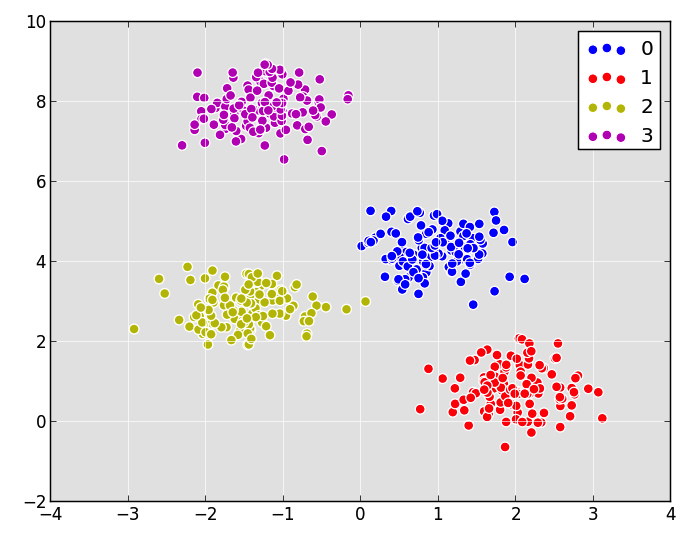
\includegraphics[width=8cm]{images/clustering.png}
	\caption{Esempio di clustering}\label{fig:clusters}
\end{figure}

In questo esempio è possibile identificare tre cluster nei quali possono essere suddivisi i dati e il criterio di similarità usato è la \emph{distanza}, quindi due oggetti fanno parte di uno stesso cluster solo se sono sufficientemente vicini tra di loro. 

\newpage

Questo tipo di clustering è detto \emph{distance-based}, ovvero basato sulla distanza. In generale, a seconda del tipo di input il problema del partizionamento si divide in:
\begin{enumerate}
	\item \textbf{feature-based:} gli oggetti sono rappresentati come vettori di caratteristiche. Nella letteratura l'algoritmo più noto è il \emph{k-means};
	\item \textbf{pairwise:} le proprietà degli oggetti sono meglio descritte in termini di \emph{similarità/dissimilarità} tra di essi. In questo caso l'input è determinato da una matrice di affinità che indica la similarità tra tutte le coppie di oggetti. Si tratta quindi di un approccio più generale rispetto al primo.
\end{enumerate}

Non sempre è facile ed intuitivo trovare un raggruppamento per i dati, come invece lo era per l’esempio visto, in quanto è difficile stabilire cosa costituisce un “buon clustering” e cosa no. In generale si può affermare che un cluster deve soddisfare i seguenti criteri:
\begin{itemize}
	\item \textbf{criterio interno}: tutti gli oggetti all'\emph{interno} di un cluster devono essere il più possibile simili tra loro;
	\item \textbf{criterio esterno}: tutti gli oggetti all'\emph{esterno} di un cluster devono essre il più possibile dissimili rispetto a quelli contenuti al suo interno.
\end{itemize}

Nelle sezioni seguenti saranno presentate alcune metodologie di clustering e ci si concentrerà, infine, sull'utilizzo della teoria dei giochi per risolvere il problema.


\newpage

\section{K-Means} % (fold)
\label{sec:k_means}
K-Means è probabilmente il più famoso algoritmo di partizionamento feature-based. Dato un insieme di osservazioni $\{x^{(1)},\dots,x^{(n)} \}$ dove $x_i$ è un vettore m-dimensionale, lo scopo dell'algortimo è partizionare l'insieme in $k$ insiemi $k \leq n$ il più possibile coesi tra loro (problema del clustering).\\

L'algoritmo seleziona a caso $k$ prototipi, rappresentanti il proprio gruppo di appartenzenza, idealmente il centro del cluster. Formalmente si ha un insieme di vettori:
\begin{align*}
	\mu_j, \text{ dove } j = 1, \dots, k
\end{align*}
L'obiettivo ora consiste nel raggruppare le osservazioni e reimpostare i vettori $\mu_j$ in modo tale che la somma del quadrato delle distanze da un punto al proprio centroide $\mu_j$ sia minima. In termini matematici si tratta di minimizzare la seguente funzione:
\begin{align}
	\min_{\{\mu_1, \dots, \mu_k\}} \sum_{i=1}^n \sum_{j=i}^k r_{ij} \| x_i - \mu_j \|^2\label{eq:j}
\end{align}
dove $r_{ij}$ è un operatore binario $r_{ij} \in \{ 0, 1 \}$. In fase di inizializzazione, si scelgono $k$ punti casuali come centri e in seguito si esegue una procedura iterativa per minimizzare \eqref{eq:j}. Ogni iterazione si compone di \textbf{due} fasi: nella prima fase (\emph{Expectation-Step}) si minimizza rispetto a $r_{ij}$ mantenendo $\mu_j$ fisso, mentre nella seconda fase (\emph{Maximization-Step}) si minimizza rispetto a $\mu_j$ mantenendo $r_{ij}$ fisso. Formalmente, nella fase E, il calcolo di $r_{ij}$ è dato da:
\begin{align*}
	r_{ij} =
	\begin{cases}
		1, &\text{ se }j = argmin_j \| x_i - \mu_j \|^2 \\
		0, &\text{ altrimenti}
	\end{cases}
\end{align*}
Intuitivamente si assegna l’osservazione $x_i$ al gruppo con $\mu_j$ più vicino.

\newpage

Nella seconda fase $\mu_k$ è dato da:

\begin{align*}
	\mu_j = \frac{\displaystyle\sum_i r_{ij} x_i}{\displaystyle\sum_i r_{ij}}
\end{align*}

Ovvero, si cerca di “spostare” al centro del cluster il prototipo $\mu_j$ come la media di tutti i punti $x_i$ assegnati al cluster $k$. Queste due fasi si ripetono fino a quando non c'è più alcuna variazione negli assegnamenti o quando un numero massimo di iterazioni è raggiunto. Infatti, trattandosi di un problema NP-Difficile non è dato sapere a priori se l'algoritmo converga oppure no.

\begin{figure}[h!]
	\centering
	\subfigure{
	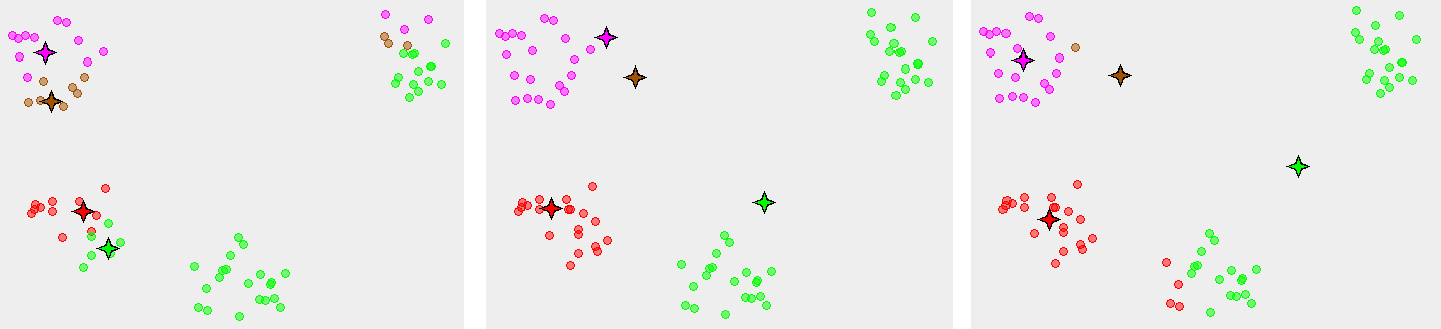
\includegraphics[width=12cm]{images/kmeans}
	}
	\subfigure{
	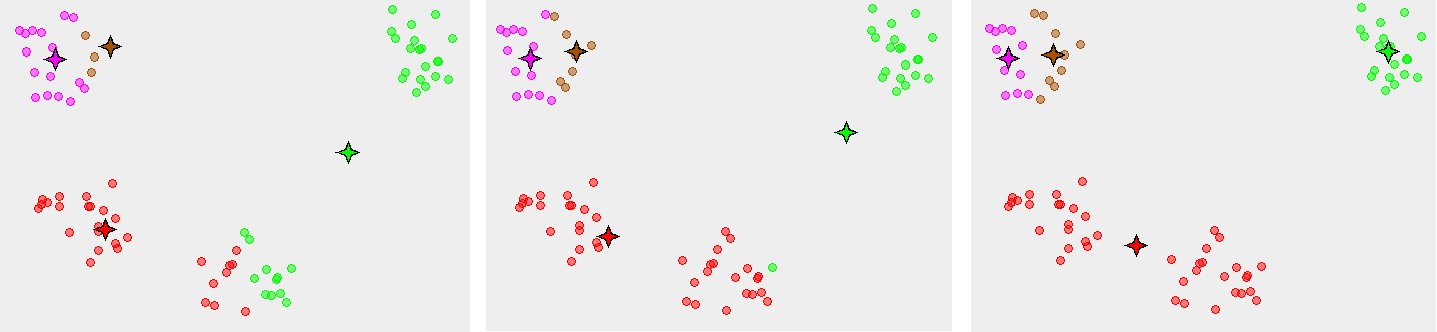
\includegraphics[width=12cm]{images/kmeans2}
	}
	\caption[Convergenza in K-means]{Esempio sulla convergenza (dopo 5 iterazioni) a un minimo locale dell'algoritmo k-means}
\end{figure}

% section k_means (end)


\section{Normalized Cut} % (fold)
\label{sec:normalized_cut}
A differenza del k-means l'algoritmo presentato in questa sezione è basato sulla teoria dei grafi e trova ampio utilizzo nella \emph{segmentazione delle immagini}, un problema analogo al clustering.
L'algoritmo \emph{normalized cut} “taglia” l'immagine utilizzando tecniche della \textbf{teoria spettrale} dei grafi. Un buon taglio divide pixel che sono dissimili tra loro. Per trovare un buon partizionamento l'algoritmo segue i seguenti passi:
\begin{enumerate}
	\item Si costruisce un grafo di similarità $G=(V, E, w)$ in cui ogni nodo rappresenta un pixel dell'immagine e il peso su ciascun arco rappresenta una misura di similarità (intensità, colore ecc..) tra ciascun pixel.
	\item Si calola il Laplaciano normalizzato definito come:
	\begin{align}
		L = D ^ {- 1 / 2} (D - A) D ^ {- 1 / 2}
	\end{align}
	dove $A$ è la matrice di adiacenza pesata e $D$ è la matrice dei gradi così definita:
	\begin{align}
		d_{i,j}:=
		\begin{cases} 
			\deg(v_i) & \mbox{if}\ i = j \\
			0 & \mbox{otherwise}
		\end{cases}
	\end{align}
	Si calcolano gli autovettori del Laplaciano normalizzato:
	\begin{align}
		L x = \lambda x
	\end{align}
	
	\item Utilizzando il segno nel secondo autovettore più piccolo (il primo è un vettore nullo) si segmenta l'immagine in due parti.

	\item La procedura si ripete ricorsivamente fino a quando si ottiene il numero desideerato di segmenti.
\end{enumerate}

L'algoritmo nella pratica si è dimostrato abbastanza efficace tuttavia il calcolo degli autovettori è un problema computazionalmente costoso: $O(n^3)$ dove $n$ è il numero di pixel. Tuttavia è possibile velocizzare l'algoritmo sfruttando il fatto che la matrice è sparsa (i valori sono quasi tutti pari a zero) ed abbassare la complessità a $O(n \sqrt{n})$\\

\begin{figure}[h!]
	\centering
	\subfigure[$original$]
	{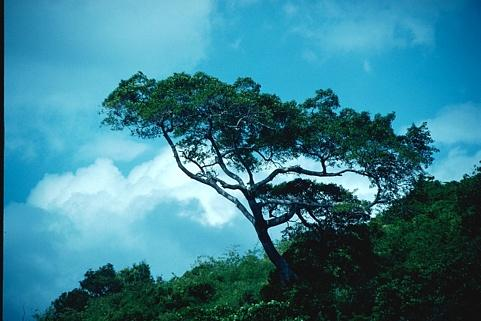
\includegraphics[width=3cm]{images/0.jpg}}
	\subfigure[$k = 2$]
	{
\includegraphics[width=3cm]{images/1.png}}
	\subfigure[$k = 3$]
	{
\includegraphics[width=3cm]{images/2.png}}
	\subfigure[$k = 4$]
	{
\includegraphics[width=3cm]{images/3.png}}
	\caption{Esempio di segmentazione ottenuta con NCUT.}
\end{figure}


% section normalized_cut (end)

\newpage


\section{Insiemi dominanti} % (fold)

Il concetto di insieme dominante nasce dallo studio sulla formulazione continua del problema della cricca massima (vedi Sezione~\ref{sec:problema_della_cricca_massima}). L'insieme dominante, infatti, non è altro che una clique di un grafo nel caso in cui gli archi siano pesati, ovvero insiemi di vertici che hanno alta omogeneità interna e alta disomogeneità verso l'esterno.\\

In questo contesto i dati sono, dunque, rappresentati da un grafo non orientato $G = (V, E , w)$ dove $V = \{ 1, \dots, n \}$ è l'insieme dei vertici, $E\subseteq V \times V$ l'insieme degli archi e $w : E \rightarrow \mathbb{R}_+$ è la funzione dei pesi positiva. I vertici rappresentano i datapoints, gli archi le relazioni tra essi e i pesi rispecchiano la similarità tra coppie di vertici connessi.\\

Come di consueto, il grafo è rappresentato con la sua matrice di adiacenza pesata $A$, che è la matrice simmetrica $n \times n$ dove $A = a_{ij}$ è definito nel seguente modo:
\begin{align*}
	a_{ij} =
	\begin{cases}
		w(i, j), &\text{ if }(i, j) \in E\\
		0, &\text{ otherwise }
	\end{cases}
\end{align*}

Si consideri $S \subseteq V$ un insieme non vuoto di vertici $i \in S$. Si introduce il concetto di \textbf{grado pesato medio} di $i$ rispetto ad $S$ definito come:\\

\begin{minipage}{.5\textwidth}
	\begin{align*}
		awdeg_S(i) = \frac{1}{|S|}\sum_{j \in S} a_{ij}
	\end{align*}
	E nel caso in cui $j \not\in S$:
	\begin{align*}
		\phi_S(i,j) = a_{ij} - awdeg_S(i)
	\end{align*}
\end{minipage}
\begin{minipage}{.5\textwidth}
	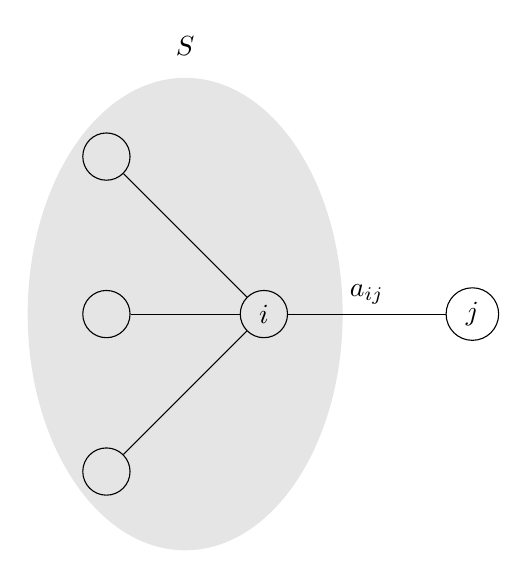
\begin{tikzpicture}[node distance=2cm]
		\fill [gray!20] (-1, 0) ellipse  (2cm and 3cm);
		\node at (-1, 3.4) {$S$};
		\node[Node] (1) at (0,0) {$i$};
		\node[Node, left of=1] (2) {};
		\node[Node, above of=2] (3) {};
		\node[Node, below of=2] (4) {};
		\node[Node, right=2cm of 1] (0) {$j$};
		\path
		(1) edge (2) edge (3) edge (4) edge[above] node{$a_{ij}$} (0)
		;
		\end{tikzpicture}\\
	\end{minipage}

	Intuitivamente $\phi_S(i, j)$ misura la similarità tra il nodo $j$ e il nodo $i$ rispetto alla similarità media tra il nodo $i$ e i suoi vicini in $S$

	\newpage

	Il peso di $i$ rispetto ad $S$ è quindi definito come:
	\begin{align*}
		w_S(i) =
		\begin{cases}
			1, &\text{ if }|S|=1\\
			\displaystyle\sum_{j \in S \setminus \{i\}} \phi_{S \setminus \{i\}} (i, j) \cdot w_{S \setminus \{i\}}(j) &\text{ otherwise}
		\end{cases}
	\end{align*}
	Si tratta di una definizione ricorsiva e permette di assegnare un peso (similarità relativa) ad ogni vertice.
	E il peso totale di $S$ è:

	\begin{minipage}{.5\textwidth}
		\begin{align*}
			W(S) = \sum_{i \in S} w_S(i)
		\end{align*}
	\end{minipage}
	\begin{minipage}{.5\textwidth}
		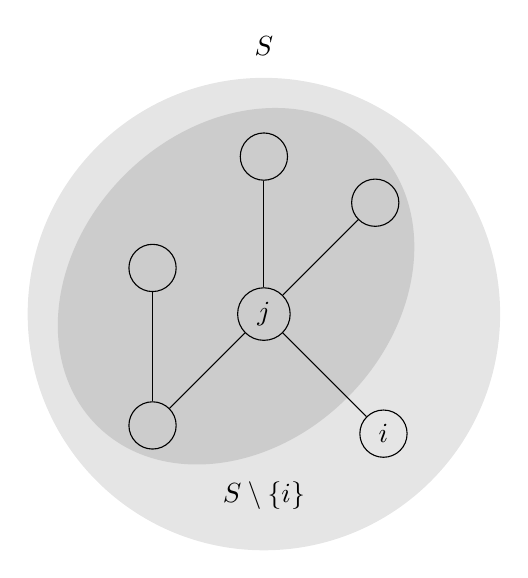
\begin{tikzpicture}[node distance=2cm]
			\fill[gray!20] (0, 0) circle  (3cm);
			\fill[gray!40, rotate=-45] (-0.5, 0) ellipse  (2cm and 2.5cm);
			\node[Node] (1) at (0, 0) {$j$};
			\node[Node, above of=1] (2) {};
			\node[Node, below left of=1] (3) {};
			\node[Node, above of=3] (4) {};
			\node[Node, below right=1.5cm of 1] (5) {$i$};
			\node[Node, above right of=1] (6) {};
			\path (1) edge (2) edge (3) edge (5) edge (6)
			(3) edge (4)
			;
		
			\node (1) at (0, 3.4) {$S$};
			\node (1) at (0, -2.3) {$S \setminus \{i\}$};
		\end{tikzpicture}
		\\
	\end{minipage}

	Intuitivamente $w_S(i)$ ci dà la misura di similarità complessiva tra il nodo $i$ e i vertici $S \setminus \{i\}$ rispetto alla similarità complessiva di ciascun vertice in $S \setminus \{i\}$. Si considerino i seguenti grafi.

	\begin{figure}[h!]
		\centering
		\subfigure[$W_{\{1,2,3,4\}(1)} < 0$]{
		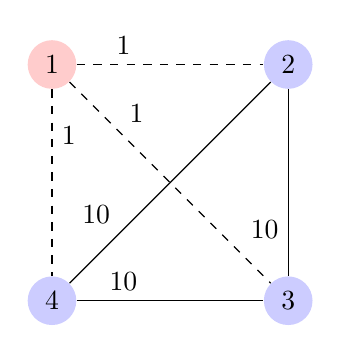
\begin{tikzpicture}[node distance=3cm]
			\node[circle,fill=red!20] (1) at (0,1.5) {1};
			\node[circle,fill=blue!20, right of=1] (2) {2};
			\node[circle,fill=blue!20, below of=1] (4){4};
			\node[circle,fill=blue!20, below of=2] (3) {3};

			\foreach \from / \to in {1/2,1/3,1/4}
			\path (\from) edge[dashed, near start, auto] node{$1$} (\to);

			\foreach \from / \to in {4/2,4/3,3/2}
			\path (\from) edge[near start, auto] node{$10$} (\to);
		\end{tikzpicture}
		}
		\qquad\qquad
		\subfigure[$W_{\{5,6,7,8\}(5)} > 0$]{
		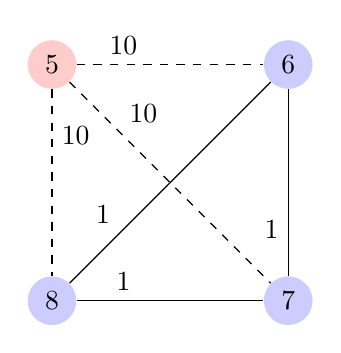
\begin{tikzpicture}[node distance=3cm]
			\node[circle,fill=red!20] (1) at (0,1.5) {5};
			\node[circle,fill=blue!20, right of=1] (2) {6};
			\node[circle,fill=blue!20, below of=1] (4){8};
			\node[circle,fill=blue!20, below of=2] (3) {7};

			\foreach \from / \to in {1/2,1/3,1/4}
			\path (\from) edge[dashed, near start, auto] node{$10$} (\to);

			\foreach \from / \to in {4/2,4/3,3/2}
			\path (\from) edge[near start, auto] node{$1$} (\to);
		\end{tikzpicture}
		}
		\caption[Insiemi dominanti e similarità]{Rappresentazione della similarità: i nodi $\{2,3,4\}$ sono altamente simili tra loro. Se si tenta di aggiungere il vertice 1 che è dissimile dalla similarità interna dell'insieme $\{2,3,4\}$ allora la similarità complessiva del nuovo insieme $\{1,2,3,4\}$ diminuisce i.e. $W_{\{1,2,3,4\}}(1) < 0$. Nel secondo caso il vertice 5 è altamente similare ai nodi $\{6,7,8\}$ di conseguenza aggiungendolo all'insieme la similarità complessiva aumenta i.e. $W_{\{5,6,7,8\}}(5) > 0$.}
	\end{figure}

	\newpage

	È stata dunque definita una misura che descrive cosa comporta (in termini di similarità) l'aggiunta o la rimozione di un nodo. Questo porta alla definizione di \emph{insiemi dominanti}.

	\begin{mydef}[Insieme Dominante]
		Un sottoinsieme di vertici non vuoto $S \subseteq V$ tale che $W(T) > 0$ per ogni insieme non vuoto $T \subseteq S$ è detto \textbf{dominante} se:
		\begin{enumerate}
			\item $W_S(i) > 0, \forall i \in S$ (omogeneità interna)
			\item $W_{S \cup \{i\}}(i) < 0, \forall i \not\in S$ (disomogeneità esterna)
		\end{enumerate}
	\end{mydef}
	L'insieme dominante è dunque un insieme di vertici massimalmente coesi tra loro e questa definizione corrisponde con quella di cluster.

	\begin{figure}[h!]
		\centering
	
		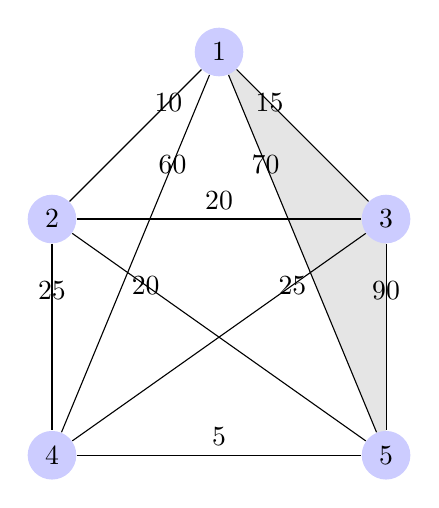
\begin{tikzpicture}[node distance=3cm]
			\node[circle,fill=blue!20] (1) at (0,0) {1};
		
			\node[circle,fill=blue!20, below left of=1] (2) {2};
			\node[circle,fill=blue!20, below right of=1] (3) {3};
        
			\node[circle,fill=blue!20, below of=2] (4) {4};
			\node[circle,fill=blue!20, below of=3] (5) {5};

			\foreach \from / \to / \label in {1/2/10,1/3/15,1/4/60,1/5/70}
			\path (\from) edge[near start] node{$\label$} (\to);
			
			\foreach \from / \to / \label in {2/4/25,2/5/20}
			\path (\from) edge[near start] node{$\label$} (\to);

			\foreach \from / \to / \label in {3/4/25,3/5/90}
			\path (\from) edge[near start] node{$\label$} (\to);

			\path (4) edge[auto] node{5} (5);
			\path (2) edge[auto] node{20} (3);

			\begin{pgfonlayer}{background}    % select the background layer
				\fill[gray!20] plot coordinates {(1) (3) (5)};
			\end{pgfonlayer}

		\end{tikzpicture}
		\caption{L'insieme $\{1,3,5\}$ è dominante.}
	\end{figure}

	Quando la matrice di affinità è binaria 0/1 allora l'insieme dominante coincide con la cricca massimale (stretta) in un grafo (vedi Sezione~\ref{sec:problema_della_cricca_massima}).\\

	\newpage

	\subsection{Insiemi dominanti e ottimi locali} % (fold)
	\label{sub:insiemi_dominanti_e_ottimi_locali}
	In questa sezione sarà mostrato come la teoria di Nash possa essere utilizzata per risolvere in modo approssimato la ricerca di insieme dominanti.\\

	Dato un grafo pesato $G = (V, E, w)$ e la sua matrice di adiacenza pesata $A$, si consideri il seguente programma quadratico standard:
	\begin{align*}
		&\text{maximize } f(x) = x^T A x\\
		&\text{subject to } x \in \Delta
	\end{align*}
	dove $\Delta$ è il simplesso standard su $R^n$. Si introduce il seguente teorema:

	\begin{thm}
		Se $S$ è un sottoinsieme dominante di vertici, allora il suo vettore caratteristico pesato $x^S$ definito come:
		\begin{align*}
			x^S_i = 
			\begin{cases}
				\frac{W_S(i)}{W(S)}, &\text{ se }i \in S\\
				0 &\text{ altrimenti}
			\end{cases}
		\end{align*}
		è un massimizzatore locale stretto di $f$ in $\Delta$.
	
		Al contrario se $x^*$ è un massimizzatore locale stretto di $f$ in $\Delta$ allora il suo supporto:
		\begin{align*}
			\sigma = \sigma(x^*) = \{ i \in V : x^*_i \neq 0 \}
		\end{align*}
		è un insieme dominante a condizione che $W_{\sigma \cup \{i\}} \neq 0$ per ogni $i \not\in \sigma$. 
	\end{thm}
	Dove la condizione $W_{\sigma \cup \{i\}} \neq 0$ è un tecnicismo dovuto alla presenza di soluzioni spurie, ovvero soluzioni che non ammettono vettore caratteristico pesato. Si tratta di una generalizzazione del teorema di Motzkin Strauss.\\

	Ora che è stata fornita una caratterizzazione di insieme dominante è possibile utilizzare una qualunque tecnica di ottimizzazione quadratica per risolvere il problema (ad esempio la discesa del gradiente). Tuttavia le dinamiche di replicazione (vedi Sezione~\ref{sec:teoria_dei_giochi_evoluzionistici}) si sono rivelate particolarmente adatte per affrontare questo problema. È stato infatti dimostrato il seguente teorema:

	\begin{thm}[Torsello, Rota Bulò, Pelillo 2006]
		Strategie evolutionary stable (ESS) di un problema di clustering con matrice di affinità $A$ sono in corrispondenza uno-a-uno con gli insiemi dominanti.
	\end{thm}

	\newpage

	Quindi sia $A$ la matrice di adiacenza del grafo di similarità. Si pone:
	\begin{align*}
		W = A (= W^T \geq 0)
	\end{align*}
	Allora un sistema di replicazione con matrice di payoff $W$ partendo da uno stato iniziale arbitrario convergerà, per il principio di selezione naturale, a un massimizzatore della funzione $f(x) = x^T A x$ nel simplesso standard. Questo corrisponderà a un insieme dominante in un grafo, ovvero ad un cluster di vertici. Quindi la ricerca di dominant sets di un grafo pesato e non orientato $G$, corrisponde a trovare equilibri di Nash asintoticamente stabili e le dinamiche di replicazione sono un ottimo strumento a disposizione per perseguire questo scopo.\\

	La teoria dei giochi evoluzionistici opera in uno scenario in cui coppie di individui sono scelti ripetutamente a caso da una grande popolazione per competere in un gioco a due giocatori. A differenza della teoria dei giochi classica, i giocatori non si comportano razionalmente ma sono pre-programmati a un certo pattern comportamentale o una strategia mista. Col passare del tempo il principio di selezione naturale inciderà sulla distribuzione dei comportamenti.\\

	Ad esempio si supponga di volere separare lo sfondo in un'immagine dagli elementi in primo piano. Nel gioco evoluzionistico ogni giocatore è pre-programmato a selezionare con una certa probabilità un elemento (un pixel) dall'immagine. In questo contesto la selezione naturale porterà giocatori che adottano strategie migliori (payoff più alto) ad espandersi, mentre quelli che adottano strategie peggiori ad estinguirsi. Nel caso descritto, ci si aspetta che la selezione naturale porti all'estinzione i giocatori che selezionano lo sfondo, per poi convergere a una popolazione che seleziona solo gli elementi in primo piano.\\

	Concludendo le caratteristiche principali che rendono questo approccio preferibile rispetto ad altri sono le seguenti:
	\begin{enumerate}
		\item Non richiede alcuna rappresentazione dei dati ovvero che gli elementi debbano essere rappresentato come punti in uno spazio vettoriale;
		\item assenza di assunzioni circa la struttura della matrice di affinità: è stato dimostrato che l'approccio funziona anche nel caso di funzioni di similarità asimmetriche o negative;
		\item non è necessaria alcuna conoscenza a priori circa il numero di clusters;
		\item permette l'estrazione di cluster sovrapposti.
	\end{enumerate}

	% subsection insiemi_dominanti_e_ottimi_locali (end)
	% section insiemi_dominanti (end)
	
	
	\section{Problema di etichettatura} % (fold)
	\label{sec:problema_di_etichettatura}
	In un tipico labelling (consistent) problem si hanno:
	\begin{itemize}
		\item $n$ oggetti $B= \{b_1, \dots, b_n\}$;
		\item $m$ etichette (labels) $\Lambda = \{\lambda_1, \dots, \lambda_m\}$.
	\end{itemize} 
	Lo scopo è assegnare a ciascun oggetto in $B$ un'etichetta in $\Lambda$.\\
	
	I legami tra oggetti ed etichette sono espressi attraverso una matrice 4-dimensionale $n^2 \times m^2$ di coefficienti di compatibilità reali $R = \{r_{ij}(\lambda, \mu)\}$: la componente $r_{ij}(\lambda, \mu)$ misura la forza di compatibilità tra le due ipotesi “$\lambda$ è sull'oggetto $b_i$” e “$\mu$ è sull'oggetto $b_j$”. Alti valori significano alta compatibilità mentre bassi valori indicano incompatibilità.\\
	
	Sia $p_i(\lambda)$ il grado di confidenza dell'ipotesi “l'etichetta $\lambda$ è sull'oggetto $b_i$”. Allora la distribuzione di probabilità delle etichette su un oggetto $b_i$ è un vettore $m$-dimensionale:
	\begin{align*}
		\bar{p}_i = (p_1 (\lambda_1), \dots, p_n(\lambda_m))^T
	\end{align*}
	con $p_i(\lambda) \geq 0$ e $\sum_\lambda p_i(\lambda) = 1$. Mettendo insieme i $\bar{p}_i$ si ottiene un \emph{assegnamento pesato delle etichette} per gli oggetti in $B$ denotato come $\bar{p}$, una matrice $n \times m$. Lo spazio degli assegnamenti pesati delle etichette è un insieme lineare convesso in $\mathbb{R}^{nm}$:
	\begin{align*}
		\mathcal{K} = \underbrace{\Delta \times \dots \times \Delta}_\textrm{$m$ times}
	\end{align*}
	dove $\Delta$ è il simplesso standard in $\mathbb{R}^n$. Ogni vertice in $\mathcal{K}$ rappresenta un assegnamento non ambiguo ovvero che assegna esattamente un'etichetta a ciascun oggetto. L'insiemi di questi labelling sarà denotato da $\mathcal{K}^*$.\\
	
	Si consideri un labelling $\bar{p} \in \mathcal{K}$. La \textbf{consistenza} di un oggetto misura il grado di confidenza tra l'ipotesi “$b_i$ è etichettato con $\lambda$” ed il contesto. Questo concetto può essere quantificato attraverso la seguente funzione di supporto lineare:
	\begin{align*}
		q_i(\lambda; \bar{p}) = \sum_j \sum_\mu r_{ij} (\lambda, \mu) p_j(\mu)
	\end{align*}
	
	\newpage
	
	Sia $p \in \mathcal{K}^*$ e sia $\lambda(i)$ l'etichetta assegnata a $b_i$ da $\bar{p}$ (i.e. $p_i(\lambda(i) = 1)$). Allora si dice che $\bar{p}$ è consistente se e solo se l'etichetta assegnata a ciascun oggetto riceve il più alto supporto da quell'oggetto. Questo corrisponde ad avere:
	\begin{align*}
		q_i(\lambda; \bar{p}) \leq q_i(\lambda(i); \bar{p})
	\end{align*}
	per ogni $i$ e $\lambda$. Applicando lo stesso ragionamento l'assegnamento pesato $\bar{p} \in \mathcal{K}$ è \emph{consistente} se:
	\begin{align*}
		\sum_\lambda v_i(\lambda)q_i(\lambda; \bar{p}) \leq \sum_\lambda p_i(\lambda) q_i(\lambda; \bar{p})
	\end{align*}
	per ogni $i = 1, \dots, n$ e $\bar{v} \in \mathcal{K}$. Inoltre se la disuguaglianza è stretta per ogni $\bar{v} \neq \bar{p}$, allora $\bar{p}$ è detto \emph{strettamente consistente}.\\
	
	Hummel e Zucker hanno dimostrato che se la matrice di compatibilità è simmetrica $r_{ij}(\lambda, \mu) = r_{ji}(\mu, \lambda)$ allora una condizione sufficiente affinché $\bar{p}$ sia consistente corrisponde a un minimo locale della seguente funzione energia che misura la (in)consistenza tra labelling:
	\begin{align*}
		A(\bar{p}) = \sum_{i, \lambda} \sum_{j, \mu} r_{ij}(\lambda, \mu) p_i(\lambda) p_j(\mu)
	\end{align*}
	
	Un processo \textbf{relaxation labelling} prende in input un assegnamento di etichette iniziale $\bar{p}^{(0)} \in \mathcal{K}$ e lo aggiusta iterativamente tenendo conto del modello di compatibilità utilizzando la seguente regola di aggiornamento:
	\begin{align}
		p_i^{(t + 1)}(\lambda) = \frac{p_i^{(t)}(\lambda) q_i^{(t)} (\lambda)}{\displaystyle\sum_\mu p_i^{(t)}(\mu) q_i^{(t)} (\mu)}\label{eq:relax}
	\end{align}
	Purchè la matrice di compatibilità sia non-negativa. Il processo evolve fino a quando non viene raggiunto un punto fisso ovvero quando $\bar{p}^{(t + 1)} = \bar{p}^(t)$. Nella pratica è solito fermare il processo quando la distanza tra due etichettamenti successivi è sotto una certa soglia oppure dopo un certo numero di iterazioni. Queste tecniche sono particolarmente utilizzate nel campo della visione artificiale.
	
	\newpage
	
	\subsection{Relaxation labelling e teoria dei giochi} % (fold)
	\label{sub:relaxation_labelling_e_teoria_dei_giochi}
	È possibile formulare un processo relaxation labelling in termini di teoria dei giochi. In questa formulazione:
	\begin{itemize}
		\item i giocatori sono gli oggetti;
		\item le etichette sono le strategie pure;
		\item gli assegnamenti pesati corrispondono alle strategia miste;
		\item la matrice di compatibilità è la matrice di payoff.
	\end{itemize}
	Pertanto un equilibrio di Nash corrisponde a un labelling consistente e un equilibrio di Nash stretto a un labelling consistente stretto. Inoltre la regola di aggiornamento~\eqref{eq:relax} corrisponde alla dinamica di replicazione utilizzata nella teoria dei giochi evoluzionistici (vedi Sezione~\ref{sec:teoria_dei_giochi_evoluzionistici}).\\
	
	Si tratta di un \textbf{polimatrix game}: un gioco non-cooperativo succinto in cui per ogni coppia di giocatori $i, j$ esiste una matrice di payoff che indica una componente del guadagno di un giocatore $i$. Il payoff totale per tale giocatore è la somma delle componenti. Formalmente:
	\begin{itemize}
		\item Ci sono $n$ giocatori con $m$ strategie;
		\item Per ogni coppia $i, j$ di giocatori c'è una matrice di payoff $A^{ij}$ di dimensione $m \times m$;
		\item Il payoff del giocatore $i$ per una certa combinazione di strategie $s_1, \dots, s_n$ è dato da:
		\begin{align*}
			\mu_i(s_1,\dots,s_n) = \sum_{j \neq i} A^{ij}_{s_i s_j}
		\end{align*}
	\end{itemize}
	Il numero di payoff per rappresentare questo gioco è $O(n^2, m^2)$. Il problema di trovare un equilibrio di Nash è PPAD-completo.
	% subsection relaxation_labelling_e_teoria_dei_giochi (end)
	% section problema_di_etichettatura (end)
	
	
	\newpage
	
	
	\section{Trasduzione di grafi} % (fold)
	\label{sec:trasduzione_di_grafi}
	La trasduzione di grafi è una popolare classe di tecniche di apprendimento semi-supervisionato che mirano a stimare la funzione di classificazione definita su un grafo in cui alcuni nodi (datapoints) sono classificati e altri no. L'idea generale consiste nel propogare in maniera consistente l'informazione appresa nei nodi etichettati a quelli non etichettati.\\
	
	Formalmente dato un insieme di datapoints $\mathcal{D} = \{\mathcal{D}_\ell, \mathcal{D}_u\}$ dove:
	\begin{itemize}
		\item $\mathcal{D}_\ell = \{(x_1, y_1), \dots, (x_\ell, y_\ell\}$ sono gli oggetti etichettati;
		\item $\mathcal{D}_u = \{x_{\ell + 1}, \dots, x_n\}$ sono gli oggetti non etichettati.
	\end{itemize}
	Le relazioni tra questi oggetti sono date da un grafo pesato non orientato $G=(V,E)$ dove i vertici rappresentano gli oggetti e gli archi misurano la similarità tra le coppie di nodi. Nel caso speciale in cui il grafo non sia pesato (la matrice di adiacenza è binaria) la presenza di un arco tra due nodi $i, j$ indica una similarità perfetta. In questo caso un cluster è dunque una componente connessa del grafo.\\
	
	\begin{figure}[h!]
	    \centering
	    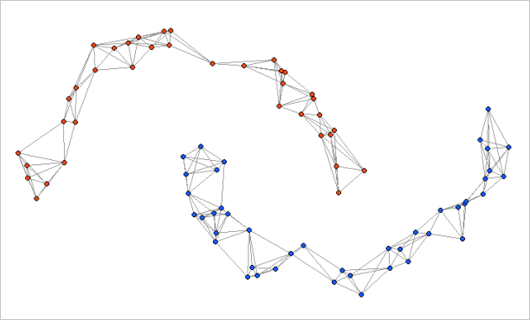
\includegraphics[width=12cm]{images/transduction}
		\caption{Apprendimento trasduttivo su un grafo non pesato.}
	\end{figure}
	
	\newpage
	
	Sia $A = a_{ij}$ la matrice di adiacenza binaria allora il problema della trasduzione su grafi non pesati può essere formalizzato come un \emph{problema di soddisfacimento di vincoli} (CSP) definito su un insieme di variabili $V = \{v_1, \dots, v_n\}$ i cui valori appartengono ai seguenti domini:
	\begin{align*}
		D_{v_i} =
		\begin{cases}
			\{y_i\}, &\text{ per ogni }1 \leq i \leq \ell\\
			Y, &\text{ per ogni }\ell + 1 \leq i \leq n\\
		\end{cases}
	\end{align*}
	e soggetto ai seguenti vincoli binari:
	\begin{align*}
		\forall i, j: \text{se } a_{ij} = 1, \text{allora } v_i = v_j
	\end{align*}
	Ad esempio in un problema a due classi i vincoli sono così definiti:
	\begin{align*}
		R_{ij} = 
		\begin{pmatrix}
			1 & 0 \\
			0 & 1
		\end{pmatrix}
	\end{align*}
	Una soluzione ad un CSP è un assegnamento di valori alle variabili che soddisfi tutti i vincoli e corrisponde ad un'etichettatura consistente per i nodi non classificati.\\
	
	È possibile risolvere un CSP con la teoria dei giochi. Si consideri il seguente gioco chiamato “\emph{graph transduction game}” (GTG). Si assuma che ogni giocatore $i \in \mathcal{I}$ corrisponda a un particolare punto nel dataset $\mathcal{D} = \{d_1, \dots, d_n \}$ e che possa scegliere una strategia nell'insieme $S_i = \{ 1, \dots, c\}$ in cui ciascuna strategia rappresenta l'ipotesi di appartenenza ad una certa classe e $c$ è il numero totale di classi.\\
	
	Per definizione del problema i giocatori sono divisi in due gruppi disgiunti:
	\begin{enumerate}
		\item \textbf{giocatori etichettati}: consapevoli della loro classe di appartenenza e denotati dall'insieme $\mathcal{I}_\ell = \{\mathcal{I}_{\ell \mid 1}, \dots, \mathcal{I}_{\ell \mid c}\}$ in cui ogni sottoinsieme $\mathcal{I}_{\ell \mid k}$ indica i giocatori che giocano sempre le loro $k$ strategie pure.
		\item \textbf{giocatori non etichettati}: $\mathcal{I}_\mu$.
	\end{enumerate}
	Ovviamente solo i giocatori non etichettati andranno a competere nel GTG in quanto i giocatori etichettati sono vincolati a giocare una strategia definita.
	
	\newpage
	
	Si suppone che in questo gioco ogni arco nel grafo rappresenti un gioco a due giocatori e quindi il payoff di ciascun giocatore è la somma dei payoff guadagnati ad ogni giocata con uno dei suoi vicini. Formalmente dato un profilo strategico misto $x = (x_1, \dots, x_n)$ la funzione di payoff di un giocatore $i \in \mathcal{I}$ è:
	\begin{align*}
		\mu_i(x) = \sum_{j=1}^n x_i^T A_{ij} x_j
	\end{align*}
	dove $A_{ij}$ è la \emph{matrice di payoff parziale} tra i giocatori $i$ e $j$. Il gioco è quindi governato dalla seguente funzione payoff:
	\begin{align*}
		\mu_i(x) = \sum_{j \in \mathcal{I}_\mu} x_i^T A_{ij} x_j + \sum_{k=1}^c \sum_{j \in \mathcal{I}_{\mathcal{D} \mid k}} x_i^T (A_{ij})_k
	\end{align*}
	Rimane ora da definire la matrice di payoff parziale. Data la matrice pesata $W = (w_{ij})$ allora la matrice di payoff parziale tra due giocatori è data da $A_{ij} = w_{ij} \times I_c$ dove $I_c$ è la matrice identità di dimensione $c$. Si noti che se la matrice di payoff parziale è rappresentata a blocchi $A = (A_{ij})$, allora la matrice $A$ è data dal prodotto di Kronecker $A = I_c \otimes W$. Ad esempio in un problema a tre classi la matrice di payoff parziale $A_{ij}$ è nella seguente forma:
	\begin{align*}
		A_{ij} =
		\begin{pmatrix}
			w_{ij} & 0 & 0 \\
			0 & w_{ij} & 0 \\
			0 & 0 & w_{ij} 
		\end{pmatrix}
	\end{align*}
	Si noti infine che nel caso di matrici di similarità binarie, allora le matrici di payoff parziale coincidono con le matrici di compatibilità definite nel CSP. Inoltre, se sono ammesse solo strategie pure allora il GTG si riduce al CSP. In questo caso in un equilibrio di Nash puro i giocatori nel vicinato giocano la stessa strategia pura con lo scopo di ottenere il payoff massimo contro i vicini. Tale equilibrio di Nash corrisponde alla soluzione del CSP se ne esiste una altrimenti il CSP è insoddisfabile e quindi il GTG non ammette equilibri di Nash.
	
% section trasduzione_di_grafi (end)
% chapter clustering (end)






















	% part teoria_dei_giochi (end)
	
	\appendix

	\part{Appendice} % (fold)
	\label{prt:appendice}
	%!TEX root = ../main.tex

\chapter{Richiami di Matematica}
\label{cha:matematica}

\section{Regole di derivazione}
\label{sec:regole_di_derivazione}

Siano $f(x)$ e $g(x)$ funzioni reali di variabile reale $x$ derivabili e sia $\mathrm{D}$ l'operazione di derivazione rispetto a $x$:
\begin{align*}
	\mathrm{D}[f(x)]=f'(x) \qquad \mathrm{D}[g(x)]=g'(x)
\end{align*}
\begin{itemize}
	\item \textbf{Regola della somma}:
	\begin{align*}
		\mathrm{D}[\alpha f(x)+ \beta g(x)] = \alpha f'(x) + \beta g'(x) \qquad \alpha, \beta \in \mathbb{R}
	\end{align*}
	\item \textbf{Regola del prodotto}:
	\begin{align*}
		\mathrm{D} [ {f(x) \cdot g(x)}] = f'(x) \cdot g(x) + f(x) \cdot g'(x) 
	\end{align*}
	\item \textbf{Regola del quoziente}:
	\begin{align*}
		\mathrm{D}\! \left[ {f(x) \over g(x)} \right] = { f'(x)  \cdot g(x) - f(x) \cdot g'(x) \over g(x)^2}
	\end{align*}
	\item \textbf{Regola della funzione reciproca}:
	\begin{align*}
		\mathrm{D}\! \left[ {1 \over f(x)} \right] = -{f'(x) \over f(x)^2} 
	\end{align*}
	\item \textbf{Regola della funzione inversa}:
	\begin{align*}
		&\mathrm{D}[f^{-1}(y)]  =  {1 \over f'(x)} \\
		&\text{con:} \\
		&y = {f(x)} \qquad x = {f^{-1}(y)}
	\end{align*}
	\item \textbf{Regola della catena}
	\begin{align*}
		\mathrm{D} \left[ f \left( g(x) \right) \right] = f' \left( g(x) \right) \cdot g'(x) 
	\end{align*}
\end{itemize}

\section{Integrali}

\begin{thm}[Teorema Fondamentale del Calcolo Integrale (prima parte)]
	Sia $f\colon [a,b]\to\mathbb{R}$ una funzione integrabile. Si definisce funzione integrale di $f$ la funzione $F$ tale che:
	\begin{align*}
		F(x)=\int_a^x f(t)dt \qquad a \le x \le b
	\end{align*}
	Se $f$ è limitata, allora $F$ è una funzione continua in $[a,b]$. 

	Se inoltre $f$ è una funzione continua in $(a,b)$, allora $F$ è funzione differenziabile in tutti i punti in cui $f$ è continua e si ha:
	\begin{align*}
		F^\prime(x)=f(x)
	\end{align*}
	cioè $F$ risulta essere una primitiva di $f$.
\end{thm}
 % Appendix A
	%!TEX root = ../main.tex

\chapter{Sistemi Dinamici} % (fold)
\label{cha:sistemi_dinamici}

Un modello matematico per descrivere le dinamiche di un sistema non lineare è lo spazio degli stati. Con questo modello si pensa in termini di variabili di stato i cui valori ad un certo istante temporale sono considerati sufficienti a predire la futura evoluzione del sistema.\\

Sia $\bar{x}(t) = x_1(t), \dots, x_N(t)$ il \textbf{vettore di stato}, un vettore contenente le variabili di stato di un sistema dinamico non lineare, in cui la variabile indipendente è il tempo $t$ e $N$ è l'ordine del sistema. È possibile allora descrivere un largo numero di sistemi dinamici non lineari mediante un sistema di equazioni differenziali di primo ordine chiamate equazioni dello spazio degli stati ed aventi la seguente forma:
\begin{align}
	\frac{d}{dt} \bar{x}(t) = F(\bar{x}(t))\label{eq:stati}
\end{align}
dove $F(\bar{x})$ è una funzione vettore che se applicata ad un vettore $\bar{x}$ ritorna un vettore che ha come j-esima componente $F_j(x_j)$ con $F_j$ una qualche funzione; si può pensare a quest'ultimo come come ad un \textbf{vettore di velocità}. Un sistema in cui la funzione vettore $F$ non dipende esplicitamente dal tempo è detto \textbf{autonomo}. In questo capitolo saranno trattati solo sistemi dinamici autonomi.\\

L'Equazione~\eqref{eq:stati} può essere vista come un descrittore del movimento di un punto nello spazio degli stati N-dimensionale; questo punto non è altro che lo stato del sistema osservato ad un certo istante $t$. Con lo scorrere del tempo il punto $t$ descrive una curva nello spazio degli stati detta \textbf{traiettoria} o orbita del sistema.

\newpage

La velocità istantanea della traiettoria è rappresentata da un vettore tangente; possiamo quindi derivare un vettore di velocità per ogni punto della traiettoria.
La famiglia delle traiettorie, per differenti condizioni iniziali, è chiamato \emph{ritratto degli stati} del sistema e comprende tutti quei punti per cui $F(\bar{x})$ è definita; nel caso di sistemi autonomi per ogni punto dello spazio esiste una sola traiettoria che vi passa.

\begin{figure}[h!]
	\centering
	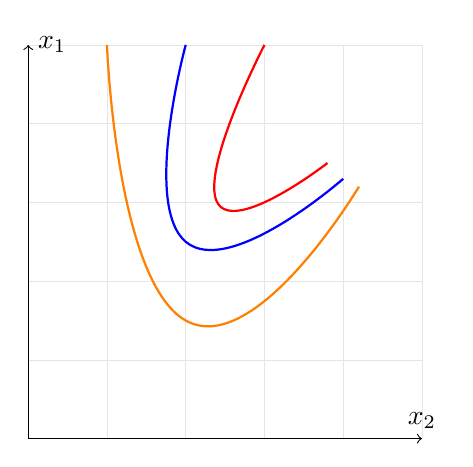
\begin{tikzpicture}
	    \draw[very thin,color=gray!20] (0,0) grid (5,5);
	    \draw[->] (0,0) -- (0,5) node[right] {$x_1$};
	    \draw[->] (0,0) -- (5,0) node[above] {$x_2$};

	    \draw[thick, color=red] plot [smooth, tension=1] coordinates{(3, 5) (2.4, 3) (3.8, 3.5)};
	    \draw[thick, color=blue] plot [smooth, tension=1] coordinates{(2, 5) (2, 2.5) (4, 3.3)};
	    \draw[thick, color=orange] plot [smooth, tension=1] coordinates{(1, 5) (2, 1.5) (4.2, 3.2)};
	\end{tikzpicture}
	\caption{Un ritratto degli stati bidimensionale di un sistema dinamico.}
\end{figure}

\section{Condizione di Lipschitz} % (fold)
\label{sub:condizione_di_lischitz}
Affinchè l’equazione dello spazio degli stati abbia soluzione e questa sia unica è necessario imporre alcune restrizioni sul vettore $F(\bar{x})$. Condizione sufficiente affinchè vi sia soluzione è che $F(x)$ sia continua in tutti i suoi argomenti; tuttavia questa condizione non garantisce l’unicità della soluzione. Serve una restrizione più forte conosciuta come condizione di Lipschitz. Una funzione:
\begin{align*}
    \mathbf{f}: \Omega \subseteq \mathbb{R}^n \rightarrow \mathbb{R}^m
\end{align*}
si dice “lipschitziana” su $\Omega$ se:
\begin{align*}
    \exists K \ge 0 
\end{align*}
tale che 
\begin{align*}
    \left \| \mathbf{f}(\mathbf{x}) - \mathbf{f}(\mathbf{y}) \right \| \le K \left \| \mathbf{x} - \mathbf{y} \right \| \qquad \forall \mathbf{x}, \mathbf{y} \in \Omega 
\end{align*}

\newpage

\begin{figure}[h!]
    \centering
    \begin{tikzpicture}[domain=-2:2]
        \begin{axis}[restrict y to domain=-2:2, grid]
            \addplot[blue,smooth,thick] function{sin(x) * cos(4 * x)} node[above=1cm] {\tiny$\sin(x)\cos(4x)$};
            \addplot[green, thick] function{- 4 * x} node[below] {\tiny$-4x$};
            \addplot[green, thick] function{4 * x} node[above] {\tiny$4x$};
        \end{axis}
    \end{tikzpicture}
    \caption{Interpretazione grafica della Condizione di Lipschitz: la funzione $f=\sin(x)\cos(4x)$ è lipschitziana con $K=4$. Ciò significa che se si considera un qualunque punto lungo la funzione e si tracciano le rette di coefficienti angolari 4 e -4, allora $f$ non sarà mai confinata tra le due rette.}
\end{figure}

% section condizione_di_lischitz (end)

\section{Stati di equilibrio} % (fold)
\label{sub:stabilità_degli_stati_di_equilibrio}
Intuitivamente un punto/stato di equilibrio stabile è un punto che non risente delle piccole perturbazioni: se ci si sposta poco da un punto stabile il sistema continuerà a rimanere anche in futuro nelle vicinanze di quel punto. L'esempio più semplice è quello di una pallina disposta esattamente nel fondo di una valle, se la spostiamo di poco dal fondo può rotolare in basso ed oscillare ma non aumenta la sua distanza dal punto di equilibrio.\\

Viceversa un punto di equilibrio instabile è tale per cui basta una perturbazione arbitrariamente piccola dall'equilibrio per far allontanare significativamente il sistema dalla posizione iniziale. Un esempio è una pallina disposta sulla cima di una collina.\\

Un vettore costante $\bar{x}\in M$ è detto stato di equilibrio (stazionario) se è soddisfatta la seguente condizione:
\begin{align*}
    \mathbf{F}(\bar{x}) = 0
\end{align*}
dove 0 è il vettore nullo. Il vettore velocità si annulla nel punto di equilibrio e quindi $\mathbf{x}(t) = x$ è una soluzione dell'equazione dello spazio degli stati. Lo stato di equilibrio è anche detto punto singolare e la traiettoria degenera nel punto stesso. Si enunciano ora una serie di definizioni sulla stabilità degli stati di equilibrio.

\begin{mydef}
    Lo stato di equilibrio $x$ è detto \textbf{uniformemente stabile} se per ogni $\bar{x}$ positivo, esiste un $\epsilon$ positivo tale che la condizione:
    \begin{align*}
        \left|\mathbf{x}(0) - \bar{x} \right| < \delta
    \end{align*}
    implica
    \begin{align*}
        \left|\mathbf{x}(t) - \bar{x} \right| < \epsilon
    \end{align*}
    per ogni $t > 0$.
\end{mydef}

Questa definizione afferma che una traiettoria del sistema può essere fatta stare in un piccolo
intorno dello stato di equilibrio $\bar{x}$ se il suo stato iniziale è vicino a $\bar{x}$.

\begin{mydef}
    Lo stato di equilibrio $x$ è detto \textbf{convergente} se esiste un $\delta$ positivo tale che la
    condizione:
    \begin{align*}
        \left|\mathbf{x}(0) - \bar{x} \right| < \delta
    \end{align*}
    implica che:
    \begin{align*}
        \lim_{t \rightarrow \infty} \mathbf{x}(t) = \bar{x}
    \end{align*}
\end{mydef}
Questa seconda definizione afferma che se lo stato iniziale di una traiettoria è adeguatamente vicino allo stato di equilibrio $x$, allora la traiettoria descritta dal vettore di stato $x(t)$ convergerà a $x$ all'aumentare del tempo.
% section stabilità_degli_stati_di_equilibrio (end)
\begin{mydef}
    Lo stato di equilibrio $\bar{x}$ è detto \textbf{asintoticamente stabile} se è stabile e convergente.
\end{mydef}
\begin{mydef}
    Lo stato di equilibrio $x$ è detto \textbf{globalmente asintoticamente stabile} se è stabile e se
    tutte le traiettorie del sistema convergono a $x$ per $t$ che tende ad infinito.
\end{mydef}

\newpage


\section{Teorema di Lyapunov} % (fold)
\label{sub:teorema_di_lyapunov}
Si enunciano ora i due teoremi di Lyapunov che forniscono condizioni sufficienti per l'esistenza di un punto stazionario.

\begin{thm}[Primo teorema di Lyapunov]
    Lo stato di equilibrio $\bar{x}$ è stabile se in un piccolo intorno di $\bar{x}$ esiste una funzione definita positiva $V(x)$ tale che la sua derivata rispetto al tempo è minore o uguale a 0 in quella regione.
\end{thm}

\begin{thm}[Secondo teorema di Lyapunov]
     Lo stato di equilibrio $\bar{x}$ è asintoticamente stabile se in un piccolo intorno di $\bar{x}$ esiste una funzione definita positiva $V(x)$ tale che la sua derivata rispetto al tempo sia strettamente minore di 0 in quella regione.
\end{thm}

Una funzione scalare $V(x)$ che soddisfa queste proprietà è detta \textbf{funzione di Lyapunov} per lo stato di equilibrio $\bar{x}$.
La funzione $V(x)$ è definita positiva nello spazio degli stati $L$, se $\forall x \in L$, soddisfa le seguenti proprietà:
\begin{enumerate}
    \item la funzione $V(x)$ ha derivate parziali rispetto agli elementi di $\mathbf{x}$ continue;
    \item $V(\bar{x})=0$;
    \item $V(x)>0$ se $\mathbf{x} \neq \bar{x}$.
\end{enumerate}

Supposta $V(x)$ una funzione di Lyapunov, lo stato di equilibrio $\bar{x}$ è stabile se:
\begin{align*}
    \frac{d}{dt} \cdot V(\mathbf{x}) \leq 0, \qquad \text{se } \left|x - \bar{x} \right| \leq \epsilon
\end{align*}
dove $\epsilon$ è un numero positivo. Lo stato di equilibrio è asintoticamente stabile se:
\begin{align*}
    \frac{d}{dt} \cdot V(\mathbf{x}) < 0, \qquad \text{se } \left|x - \bar{x} \right| \leq \epsilon
\end{align*}

Il criterio è una generalizzazione del fatto, ben noto nella fisica, che un sistema meccanico, se lasciato libero di evolvere, tende a portarsi in una configurazione dove la sua energia potenziale è minima. La funzione di Lyapunov può quindi essere interpretata come una funzione di energia potenziale generalizzata. Il criterio dice che uno stato di equilibrio è stabile se:
\begin{enumerate}
    \item è minimo per una certa funzione di energia generalizzata (cioè se esiste una funzione di Lyapunov definita positiva);
    \item se il sistema tende a portarsi verso la configurazione di minimo della funzione di Lyapunov (cioè se la derivata della funzione di Lyapunov è semidefinita negativa).
\end{enumerate}
Il criterio è una \textbf{condizione sufficiente ma non necessaria}. Non è detto in generale che l'origine non sia stabile se non esiste una funzione di Lyapunov definita in un intorno dell'origine. Inoltre non esiste un algoritmo per trovare la funzione di Lyapunov relativa a un sistema, ma si deve cercare per tentativi, basandosi sul tipo di funzione di stato e su considerazioni puramente fisiche.

% section teorema_di_lyapunov (end)
% chapter sistemi_dinamici (end)
 % Appendix B
	% part appendice (end)

	\cleardoublepage% Bibliography
\nocite{*}
\label{app:bibliography} % Reference the bibliography elsewhere with \autoref{app:bibliography}

\manualmark
\markboth{\spacedlowsmallcaps{\bibname}}{\spacedlowsmallcaps{\bibname}} 
\refstepcounter{dummy}

\addtocontents{toc}{\protect\vspace{\beforebibskip}} % Place the bibliography slightly below the rest of the document content in the table of contents
\addcontentsline{toc}{chapter}{\tocEntry{\bibname}}

\bibliographystyle{plainnat}

\bibliography{bibliography}

\end{document}
